\documentclass[11pt,twoside,openany]{book}

\usepackage{verbatim}
\usepackage{algpseudocode}
\usepackage{algorithm}
\usepackage{graphicx}
\usepackage{geometry}
\PassOptionsToPackage{hyphens}{url}
\usepackage[allcolors=blue,colorlinks=true,breaklinks]{hyperref}
\usepackage{url}
\usepackage{enumerate}
\usepackage{latexsym,booktabs}
\usepackage{amsmath,amssymb}
\usepackage{graphicx}
\usepackage[singlespacing]{setspace}
\usepackage{placeins}
\usepackage{minted}
\usepackage[round]{natbib}
\usepackage{siunitx}
\geometry{a4paper,left=2cm,right=2.0cm, top=2cm, bottom=2.0cm}
\sisetup{output-exponent-marker=\ensuremath{\mathrm{e}}}

%headers
\newcommand{\citeay}[1]{\citeauthor{#1},~\citeyear{#1}}
\newcommand{\eps}{\varepsilon}
\newcommand{\code}[1]{\mintinline{text}{#1}}
\let\oldvec=\vec{}
\renewcommand{\vec}[1]{\boldsymbol{#1}}
\newcommand{\norm}[1]{\left\lVert#1\right\rVert}
\newcommand{\p}{\mathbb{P}}
\newcommand{\prob}{\mathbb{P}}
\newcommand{\dee}{\mathrm{d}}
\newcommand{\delby}[2]{\frac{\partial #1}{\partial #2}}
\newcommand{\dby}[2]{\frac{\partial #1}{\partial #2}}
\newcommand{\dx}{\mathrm{d}x}
\newcommand{\e}{\mathrm{e}}
\newcommand{\E}{\mathbb{E}}
\newcommand{\I}{\mathcal{I}}
\newcommand{\nat}{\mathbb{N}}
\newcommand{\Z}{\mathbb{Z}}
\renewcommand{\H}{\mathcal{H}}
\newcommand{\md}{\mathrm{d}}
\newcommand{\cov}{\text{cov}}
\newcommand{\var}{\text{Var}}
\newcommand{\reals}{\mathbb{R}}
\newcommand{\R}{\mathbb{R}}
\newcommand{\C}{\mathbb{C}}
\newcommand{\D}{\mathcal{D}}
\newcommand{\ra}{\rightarrow}
\DeclareMathOperator*{\argmin}{arg\!min}
\DeclareMathOperator*{\argmax}{arg\!max}
%\newcommand{\expnumber}[2]{{#1}\mathrm{e}{#2}}


\newtheorem{Definition}{Definition}
\newtheorem{Theorem}{Theorem}
\newtheorem{Lemma}{Lemma}
\newtheorem{Corollary}{Corollary}
\newtheorem{Proposition}{Proposition}
\newtheorem{Algorithm}{Algorithm}
\numberwithin{Theorem}{chapter}
\numberwithin{Definition}{chapter}
\numberwithin{Lemma}{chapter}
\numberwithin{Algorithm}{chapter}
\numberwithin{equation}{chapter}

% avoid empty appendix page
%\makeatletter\@openrightfalse\makeatother


% *********************************************************************
% Headings and page layout
% *********************************************************************
\usepackage{fancyhdr} % to design my own headings
\usepackage{titlesec, titletoc} % to design my own toc and part/chapter/section styles

% page style of "chapter"
\titleformat{\chapter}[display]{\LARGE \bfseries}
	{\Large Chapter \thechapter \thispagestyle{plain}}{0ex}{\titlerule\vspace{2ex}}
\titlespacing*{\chapter}{0ex}{-8ex}{8ex}

% definition of headings
\fancypagestyle{memo}{
	\pagestyle{fancy}
	\fancyhf{}
	\fancyhead[RO,LE]{\thepage}
	\fancyhead[RE]{\rightmark}
	\fancyhead[LO]{\leftmark}
	\renewcommand\headrulewidth{0.5pt}
}

\begin{document}

\pagestyle{empty}

% =============================================================================
% Title page
% =============================================================================
\begin{titlepage}
\vspace*{.5em}
\center
\textbf{\large{The School of Mathematics}} \\
\vspace*{1em}
\begin{figure}[!h]
\centering

\includegraphics[width=180pt]{CentredLogoCMYK.jpg}
\end{figure}
\vspace{2em}
\textbf{\Huge{Conditional extreme value mixture models and their application
to stationary time series}}\\[2em]
\textbf{\LARGE{by}}\\
\vspace{2em}
\textbf{\LARGE{Ben Anson}}\\
\vspace{6.5em}
\Large{Dissertation Presented for the Degree of\\
MSc in Statistics and Operational Research}\\
\vspace{6.5em}
\Large{August 2022}\\
\vspace{3em}
\Large{Supervised by\\Dr. Ioannis Papastathopoulos}
\vfill
\end{titlepage}

\cleardoublepage


% =============================================================================
% Abstract, acknowledgments, and own work declaration
% =============================================================================
\begin{center}
\Large{Abstract}
\end{center}

Extreme value theory provides general results regarding the asymptotics of
probability distribution functions that can be leveraged by statisticians to
perform out-of-sample inference. This inference tends to be more difficult in a
multivariate setting, but tools have been developed to combat the multivariate
case, such as conditional extreme value models. In this dissertation, we explore
the use of conditional extreme value mixture models (CEVMMs) for modelling
tail switching behaviour of stationary time series.
An EM algorithm for fitting  CEVMMs is developed and its efficacy
illustrated on data generated from an asymmetric logistic model.
It is then shown that UK electricity imbalance prices exhibit tail switching
behaviour and that CEVMMs are able to model this. Furthermore,
it is demonstrated that CEVMMs are able to produce convincing one-step-ahead
predictive distributions for imbalance price residuals.



%We present a method for modelling tail switches in stationary time series, that
%seeks asymptotic modes in the joint distribution of 2 or more consecutive
%observations. The method
%takes advantage of developments in multivariate extreme value theory,
%with particular inspiration from the Heffernan-Tawn model. A simulation study
%is performed to investigate its efficacy on 2nd order Markov processes.
%Finally, the procedure is applied to Elexon electricity imbalance price data.

\clearpage

\begin{center}
\Large{Acknowledgements}
\end{center}

Thank you to Ioannis, for the many hours spent explaining some of the finer
details of the statistics of extremes, and of statistics and probability in
general. I left every meeting with fresh problems, new ideas to try, and of course a
thick wad of paper covered head to toe with scribbles.

\clearpage

\begin{center}
\Large{Own Work Declaration}
\end{center}

I declare that the following work is my own, except where otherwise stated.



%\cleardoublepage
\clearpage



% =============================================================================
% Table of contents, tables, and pictures (if applicable)
% =============================================================================
\pagestyle{memo}

\setcounter{page}{1}
\pagenumbering{Roman}

% Table of contents
\thispagestyle{plain}
\tableofcontents
\clearpage

\thispagestyle{plain}
\hrule
\chapter*{Notation}

\subsection*{Mathematical}
\begin{tabular}{lp{\textwidth}}
  $\reals_{+}$ & $\{x\in\reals\,|\,x > 0\}$ \\
  $\mathcal{S}_K$ & $\left\{x\in\reals^K\,\middle |\, x \geq 0,\,\sum_{k=1}^K x_k = 1\right\}$, the $K-1$ dimensional simplex \\
  $(x)_+$ & $\max\{x, 0\}$ \\
  $x_{\{i_1,\,\ldots,\,i_m\}}$, where $x\in\reals^d$ & $(x_{i_1},\,\ldots,\,x_{i_m})$ \\
  $x_{\{i_1,\,\ldots,\,i_{m}\},\,\ldots,\,\{j_{1},\,\ldots,\,j_{m'}\}}$ & $(x_{i_1},\,\ldots,\,x_{i_m},\,\ldots,\,x_{j_{1}},\,\ldots,\,x_{j_{m'}})$ \\
  $x_{/i}$, where $x\in\reals^d$ & $(x_1,\,\ldots,\,x_{i-1},\,x_{i+1},\,\ldots,\,x_d)$ \\
  $\text{sigmoid}(x)$ & $[1 + \exp(-x)]^{-1}$ \\
  $\text{logit}(x)$ & $\log\left[x/(1-x)\right]$ \\
  $X_{1:t}$ & $\{X_1,\,\ldots,\,X_t\}$ \\
  $\hat F_{\text{ecdf}}$ & Empirical cumulative distribution function \\
  $f(\cdot\,;\,\theta)$ & $f:X\rightarrow Y$ with $f(x;\theta) = g(x,\theta)$ for some $X$, $Y$ and $g : X \times \Theta \rightarrow Y$\\
  $1(\cdot)$ & Indicator function\\
  $F_{0}(x)$ & $\prob(X_0 \leq x)$\\
  $F_{1|0}(x;x_0)$ & $\prob(X_1 \leq x\,|\, X_0 = x_0)$\\
  $F_{2|1,0}(x;x_1,x_0)$ & $\prob(X_2 \leq x\,|\,X_1=x_1,\, X_0= x_0)$\\
\end{tabular}\\
\subsection*{Nomenclature}
\begin{tabular}{lp{\textwidth}}
  LHS & Left hand side \\
  RHS & Right hand side \\
  CDF & Cumulative distribution function \\
  ECDF & Empirical cumulative distribution function \\
  MCMC & Markov chain Monte Carlo \\
  MISE & Mean integrated square error \\
  MIAE & Mean integrated absolute error \\
  i.i.d.\ & Independent and identically distributed \\
  r.v.\ & Random variable \\
  EVT & Extreme value theory \\
  GPD & Generalized Pareto distribution \\
  CEVMM & Conditional extreme value mixture model
\end{tabular}\\

\clearpage

% Table of tables (if applicable)
\thispagestyle{plain}
\listoftables
\clearpage

% Table of pictures (if applicable)
\thispagestyle{plain}
\listoffigures
\clearpage

\thispagestyle{plain}
\listofalgorithms
\clearpage

\pagenumbering{arabic}
\setcounter{page}{1}





%\nocite{*}
%\bibliographystyle{apa}
\bibliographystyle{plainnat}
\cleardoublepage % always start a new chapter on an odd page

\chapter{Introduction}\label{sec.intro}

Extreme value theory (EVT) is concerned with quantifying uncertainty around
unlikely events. This is an intrinsically difficult task because,
by definition, one usually has little data regarding an extreme event.
Unfortunately, the naive approximation for the probability of an extreme
event (namely 0) is sometimes insufficient. Accordingly, EVT has been an active area
of research and it is commonly applied to areas such as
finance~\citep{embrechts1999extreme,gilli2006application,gkillas2018application} and
the environmental sciences~\citep{katz1999extreme,towler2010modeling}.

In this dissertation, we are interested in the methodologies that
can be derived from EVT. In particular, we look at the development and application of an EM
algorithm for conditional extremes  of multivariate
data. Conditional extreme value mixture models (CEVMMs) are a statistical construct, and
require only a fairly mild assumption about the distribution $F$ that generates
the data being modelled. If a random $d$-vector $X$ is
distributed according to $F$, then we assume that
\[
  \prob\left(\frac{X_{/j} - b(x)}{a(x)} \leq z\,\middle|\,X_j = x\right)\rightarrow G(z) \text{ as } x\rightarrow\infty,
\]
where $G$ is a non-degenerate probability distribution. This assumption
originates from the seminal paper by~\cite{heffernan2004conditional}, where a
methodology was developed for modelling the unknowns $G$, $a$ and $b$. Their
methodology has been extended and improved since
then~\citep{keef2013estimation}. The methodology is
semi-parametric, in that parametric assumptions are made in order to find
estimates of the functions $a$ and $b$, and then nonparametric methods are used
to model $G$. There is a subtle complication in that the functions
$a$ and $b$ are not necessarily unique, but this naturally leads to use
of mixture models where each mixture component accounts for a unique combination
of the functions $a$ and $b$. CEVMMs are based on this mixture model assumption.

In what is believed to be a novel development, we apply these mixture models to
univariate stationary time series $\{X_t\}_{t\in \{1,\,\ldots,\,n\}}$. We do
this by first viewing the time series as a set of consecutive pairs $\D' =
\{(X_{t},X_{t+1})\,|\,t\in\{1,\,\ldots,\,n-1\}\}$. Then, assuming that
the subset of pairs where the first element is large is a sample
of i.i.d.\ draws from the same distribution, a CEVMM model can be fit
to characterize the tail switching properties of $X_t$.
Although an i.i.d.\ assumption is unreasonable in general, it is more palatable
here since if $n$ is large enough, other dependent variables will in effect be
integrated out.

The structure of this dissertation proceeds as follows. In
Section~\ref{sec:background} a brief overview of EVT and two of
its important results are given,
as well as an explanation of the origins of the crucial
assumptions and methods developed in~\cite{heffernan2004conditional}. The
concept of tail switching is also introduced. Next, in Section~\ref{sec:methods}, we show how CEVMMs can be fitted
on simulated asymmetric logistic data viewed as a Markov chain, and we illustrate
how uncertainty can be quantified. With the knowledge gained from working with
simulated data, we apply CEVMMs to electricity imbalance price residuals.
We show that CEVMMs are able to capture conditional extremal dependence of these
residuals, and also offer convincing predictive distributions for
the next residual.
Finally, in Section~\ref{sec:conclusion}, the results are summarised and suggestions for future work are put forward.

%CEVMMs are an unfortunate consequence of the fact that
%Extreme value theory (EVT) and CEVMMs exist because there is a
%demand for tools for managing the risk of rare events.
%In this dissertation, we apply EVT to heavy tailed univariate time series that
%exhibit `tail switching'. EVT inspired models for the tails of these time
%series give us the ability to characterise tail behaviour and estimate
%quantities such as switching probabilities and expected time in the tails.
%Specifically, we first demonstrate the efficacy of our models on asymmetric
%logistic data (whose properties have been studied,
%e.g.~\cite{coles1991modelling}), and then provide an analysis of electricity
%imbalance price data.\\

%TODO drawbacks of mixture models



\clearpage % always start a new chapter on an odd page


\chapter{Background}
\label{sec:background}


\section{Univariate extremes}

Crucial components of EVT are the
Fisher-Tippet-Gnedenko Theorem~\citep{coles2001introduction}, and the closely
related Pickands-Balkema-de Haan
Theorem \citep{balkema1974residual,pickands1975statistical}. These
asymptotic results give justification for extrapolating beyond data
in a principled way, first pioneered in~\cite{davison1990models}. This can be
very powerful, and we approach the subject with this as our goal.

\begin{Theorem}\normalfont{(Pickands–Balkema–de Haan)}
  \label{thm:pbdhtheorem}\\
  Let $X$ be an r.v.\ with cumulative distribution $F$.
  Then if there exist $a(u) \in \mathbb{R}_{+}$, $b(u)\in\mathbb{R}$,
  and $G$ non-degenerate such that
  \[
    \mathbb{P}\left(\frac{X - b(u)}{a(u)}\leq z\,\middle|\,X>u\right)\rightarrow G(z)
    \text{ as }{u\rightarrow \infty},
  \]
  then $G$ is a Generalized Pareto Distribution (GPD) function parameterized
  by $\xi \in \reals$ such that
  \[
    G(z) = G(z;\xi)= 1 - \left(1 + \xi z\right)_{+}^{-1/\xi}.\\
  \]
\end{Theorem}

Theorem~\ref{thm:pbdhtheorem}
allows for a natural application in distribution estimation. Given
$\{X_i\}_{i=1}^n$ that are assumed to be i.i.d.\ drawn from an unknown distribution
$F$, Theorem~\ref{thm:pbdhtheorem} motivates the following method for estimating $F$ in
its upper tail with a GPD distribution $G$
\begin{equation}\label{eq:fhat_univariate}
  \hat F(z) = G((z - \hat b)/\hat a\,;\, \hat\xi)  \text{ for } z > v.\\
\end{equation}
The parameters $a$, $b$, $\sigma$ and $\xi$ can be fit via some statistical
procedure (e.g.\ maximum likelihood) on a set of exceedances $\{X_i\,|\, X_i >
v,\,i\in\{1,\,\ldots,\,n\}\}$. A more standard estimator can be used to
estimate $F(z)$ for $z < v$, such as
the ECDF.
Finding a suitable $v$ can be troublesome
as its selection corresponds to a bias-variance trade-off~\citep{coles2001introduction}.
However, given a sufficient amount of data it is generally possible to
fit such a model and therefore allow for extrapolation in the tails.
Relatively mature software packages exist for fitting these models and quantifying confidence
intervals (see for example~\citeay{mev}), so analyses of this kind should be considered
approachable.

\section{Multivariate extremes}

In the univariate case, we have univariate extreme value distributions,
which give rise to the useful Pickands-Balkema-de Haan Theorem~(\ref{thm:pbdhtheorem}).
In the multivariate case, we have the following Theorem~\ref{thm:mvextypes} concerning
multivariate extreme value distributions, stated assuming Fréchet margins.
Restricting to Fréchet margins is not limiting, since we can
transform data to/from any margin via $ Q \circ \hat F$, where $Q$ is the relevant
quantile function.

\begin{Theorem}\normalfont{(Multivariate Extremal Types)}\label{thm:mvextypes}\\
  Let $\{X^i\}_{i=1}^n=\{(X^i_1,\,\ldots,\,X^i_d)\}_{i=1}^n$ be independent
  random $d$-vectors with unit Fréchet marginals. Let $M^n\in \mathbb{R}^d$ be
  the vector of component-wise maxima, so that $M^n_j = \max_{i=1}^n
  X^i_j$.
  Take the following vector additions, multiplications, etc.\ to be component-wise,
  and read $a<b,\,a,\,b\in\mathbb{R}^d$ to mean that $a_i < b_i,\,\forall
  i\in\{1,\ldots,\,d\}$.
  Suppose there exist $a_n \in \mathbb{R}_{+}^d$, $b_n\in\mathbb{R}^d$ and
  non-degenerate $G$ such that
  \[
    \mathbb{P}\left(\frac{M^n - b_n}{a_n}\leq z\right)\rightarrow G(z) \text{ as } {n\rightarrow \infty}.
  \]
  Then for any pair of norms $\norm{\cdot}_1$, $\norm{\cdot}_2$ on $\reals^d$, $G$ can be
  written in the following form
  \[
  \begin{aligned}
    G(z) &= \exp\left[-V(z)\right],\\
    V(z) &= \int_{\Xi} \max_{j\in\{1,\,\ldots,\,d\}}\left\{\frac{\omega_j}{\norm{\omega}_1}\frac{1}{z_j}\right\} S(\md \omega),\\
  \end{aligned}
  \]
  where $\Xi = \{\omega\in\reals^d : \norm{\omega}_2 = 1,\,\omega \geq 0\}$ and
  $S$ is a measure over the Borel sets $\mathcal{B}(\Xi)$ satisfying
  $\int_{\Xi}\omega_j/\norm{\omega}_1 S(\md \omega)=1$ for all
  $j\in\{1,\ldots,\,d\}$.\\
\end{Theorem}

If it were possible to establish $V$ in Theorem~\ref{thm:mvextypes}, as well as
the normalizing constants $a_n$, $b_n$ for some multivariate
data, then
in principle it should be possible to form a multivariate equivalent
of the distribution estimator in~\eqref{eq:fhat_univariate} for large $n$,
by approximating $F$  as follows
\[
  \begin{aligned}
  \prob((M^n -  b_n)/ a_n\leq  z) &\approx \exp\left[-V( z)\right]\\
    \implies F(a_n  z +  b_n)^n &\approx \exp\left[-V( z)\right] \text{ assuming $X_i$ i.i.d.}\\
    \implies F(  z ) &\approx \exp\left[-\frac{1}{n}V\left(\frac{z - b_n}{a_n} \right)\right].\\
  \end{aligned}
\]
Notice, however, that $V$ is characterized by a measure $S$, which makes
inference very difficult.
Parametric models~\citep{tawn1990modelling}
as well as nonparametric models~\citep{marcon2017multivariate}
for $V$
have been proposed,
but ultimately there is no
general and statistically practical multivariate equivalent of
Theorem~\ref{thm:pbdhtheorem} that allows for multivariate density estimation/extrapolation in
the tails.

\section{Conditional extreme value models}

Suppose we have $n$ i.i.d.\ random $d$-vectors
$\{X^i\}_{i=1}^n = \{(X^i_1,\,\ldots,\,X^i_d)\}_{i=1}^n$.
We drop the $i$ superscript for notational convenience from here. We have
established that it is difficult to estimate $\prob(X > u + z\,|\,X > u)$
for some extreme $u$ using the multivariate value distributions from
Theorem~\ref{thm:mvextypes}. \cite{heffernan2004conditional} propose an
alternative method for modelling the extremal dependence of multivariate data.
Instead of considering $\prob(X> u + z\, |\, X > u)$ directly, consider
$\prob(X_{/j} > u + z\, |\, X_j = x_j)$, for all $j\in \{1,\ldots,d\}$.
To see why this is worthwhile, note that
the latter can be used to find the former. For example, in the case $d=2$,
\begin{equation}\label{eq:thresh_to_ht}
    \prob(X > u + z\,|\,X > u)
  = \frac{1}{1-F_2(u_2)}\int_{x_1 > u_1+z_1} \prob(X_2 > u_2 + z_2\, |\, X_1 =x_1)f_{1}(x_1)\md x_{1},
  \end{equation}
where $F_2$ is the distribution of $X_2$ and $f_1$ is the density
of $X_1$. Assuming we have a model for $\prob(X_2 > u_2 + z_2\, |\, X_1 = x_1)$, then the
RHS of~\eqref{eq:thresh_to_ht} can be used to estimate the LHS. Whilst
the denominator is also unknown, we can estimate it
using univariate results such as~\eqref{eq:fhat_univariate}, or with a simple
empirical proportion. Similarly
the integral is intractable, but can be estimated using Monte Carlo methods.
All that remains is an approach to modelling such quantities as
$\prob(X_{/j}> u + z |X_j = x)$. We assume that there exist
normalizing constants $a(x)>0$, $b(x)$, and some non-degenerate $G$ such that
\begin{equation}
  \label{eq:htassump}
  \prob(X_{/j} - b(x))/a(x)\leq z \,|\,X_j = x)\rightarrow G(z) \text{ as } {x\rightarrow\infty}.
\end{equation}
This suggests that the following approximation is appropriate
\begin{equation}
  \label{eq:basichtapprox}
\prob\left(X_{/j}\leq y\middle| X_{j} = x\right)\approx
G\left(\frac{y - b(x)}{a(x)}\right),
\end{equation}
and indeed this is what~\cite{heffernan2004conditional}
studied. In practice,
the functions $a$ and $b$ are not necessarily unique, and there can
be several combinations of functions that yield non-degenerate limits in~\eqref{eq:htassump}.
This has been explored
by~\cite{tendijck2021modeling}, and
we can make~\eqref{eq:basichtapprox} more general with the following approximation
\begin{equation}\label{eq:modalhtapprox}
  \prob\left(X_{/j}\leq y\middle| X_{j} = x\right)
  \approx \sum_{k=1}^K \pi_k G_k\left(\frac{y - b_k(x)}{a_k(x)}\right)
\text{ for large }x,
\text{ with }(\pi_1,\,\ldots,\,\pi_K)\in \mathcal{S}_{K},
\end{equation}
where $K$ is the number of `modes' (equivalently the number of unique
combinations of suitable normalization functions), and $\mathcal{S}_K$ is the
probability simplex with dimension $K-1$. We will focus
heavily on fitting models of kind~\eqref{eq:modalhtapprox}.

\FloatBarrier

\section{Fitting conditional extreme value mixture models (CEVMMs)}

If all of $K$, $a_k$, $b_k$ and $G_k$, for $k=1,\ldots,K$, are known
then
fitting the model~\eqref{eq:modalhtapprox} is straightforward because
the RHS becomes a simple mixture model of known distributions.
Algorithmic options for fitting the mixture weights include
\begin{enumerate}[(a)]
  \item EM --- there are
    closed form solutions to the parameter updates for $\pi$, and EM is known
    to converge
    to the MLE for $\pi$~\citep{redner1984mixture};
  \item Bayesian methods --- a Dirichlet prior for $\pi$ yields
    closed form updates in a Gibbs sampler~\citep{li2019tutorial} because
    it is a conjugate prior for the Multinomial distribution.
\end{enumerate}
Unfortunately in practice, given real data, none of the parameters or
distributions will be
known. We will not even know the number of modes. There is a history of workarounds for this issue.
In their original paper,~\cite{heffernan2004conditional}
proposed transforming data to Gumbel margins, and then using $a(x) = x^\beta$
and $b(x) = \alpha x + 1(\alpha=0,\beta < 0)\cdot(\gamma - \delta \log (x))$
in~\eqref{eq:modalhtapprox}. This parametric family was motivated by
the fact that it fits with many types of dependence structures/copula.
However, a similar, but simpler form for $a$ and $b$
was suggested in~\cite{keef2013estimation}.
Using Laplace margins instead yields $a(x) = x^\beta$ and $b(x) = \alpha x$
for a large class of copula.
Laplace margins have a further advantage over Gumbel margins in that
an extreme value analysis can be performed easily in both the lower and the upper tails
because the Laplace density is symmetric.
Secondly, it has been common to use ECDF in place of the $G_k$'s.
It is not possible to fit $\alpha$'s, $\beta$'s and $\pi$ under this
assumption, and so classically for the fitting step a false working assumption
that the $G$'s are normally distributed has been used. It is stressed that once
estimates for the mixture weights and the normalization constants are found,
the normal assumption is dropped. Putting these workarounds together yields the
following model for the fitting step
\begin{equation}\label{eq:ht_mix_fitting_step}
  \prob\left(X_{l}\leq y\middle| X_{j} = x\right) = \sum_{k=1}^K \pi_k \Phi\left(\frac{y - \alpha_k x}{x^{\beta_k}}\,;\,\mu_k,\sigma_k^2\right) \text{ for large } x,\, l\in\{1,\,\ldots,\,d\},\,l\neq j,
\end{equation}
where $\Phi$ is the univariate normal CDF. For the $d=2$ case,
fitting~\eqref{eq:ht_mix_fitting_step} requires data $\D' =
\{(x_i,y_i)\}_{i=1}^n$, where $(x_i , y_i)$ are assumed to be i.i.d.. It is
necessary to select a cut-off $u>0$ and fit using $\D = \{(x,y)\in \D' \,|\, x
> u\}$ so that the `large $x$' constraint is satisfied. This is analogous to
the choice of $v$ in~\eqref{eq:fhat_univariate}, and the selection of $u$ also
corresponds to a variance/bias trade-off. Once parameter estimates have been
found, let $C_i\in\{1,\,\ldots,\,K\}$ be the classification of each pair
$(x_i,y_i)\in\D$. By sampling $C_i$ many times, we can construct sets of
residuals $Z_1,\,\ldots,\,Z_K$, where $(y_i - \alpha_k x_i)/x_i^{\beta_k}$ is
added to $Z_k$ every time $k$ is sampled from $C_i$. Finally, we can drop the
normal assumption and construct ECDFs for each of these sets of
residuals, yielding the final model
\begin{equation}\label{eq:ht_mix_final}
\prob\left(X_{l}\leq y\,\middle|\, X_j = x\right) \approx
\sum_{k=1}^K\hat\pi_k \hat F^k_{\text{ecdf}}\left(\frac{y - \hat\alpha_k
x}{x^{\hat\beta_k}}\right) \text{ for large }x.
\end{equation}
The business of fitting model~\eqref{eq:ht_mix_fitting_step} is not simple ---
even though it is a mixture of Gaussians, it is not amenable to techniques for
fitting Gaussian mixture models because the CDFs permit an argument that
is non-linear in the data $x$.
No closed form solution exists (nor are there a closed form solutions to
parameter updates if an EM algorithm is applied). Adaptive MCMC has been used
previously~\citep{tendijck2021modeling}, but here we consider an EM algorithm
which is explained in depth in
the~\hyperref[appendix:htnormalem]{appendix}.

\section{Tail switching}

We briefly introduce the concept of tail switching, and discuss its relevance in
terms of conditional extreme value models.
We say that a time series $\{X_t\}_{t\in \mathbb{Z}}$ tail
switches if
for some fixed large threshold $u$,
$X_{t} > u > X_{t+1}$. In other words, a series tail switches if it moves from
the upper tail of its distribution to the main body. It is necessary to assume
some degree of stationarity for
$X_t$, as otherwise $u$ may need to vary with $t$.

There are many examples of tail switching series in practice:
see Figure~\ref{fig:sap500ts} which shows several tail switches of S\&P log returns
(on the Laplace scale), along with the actual price.
The log return transformation is necessary as it serves to residualize the
data (so that it is stationary).
\begin{figure}[htp]
  \centering
  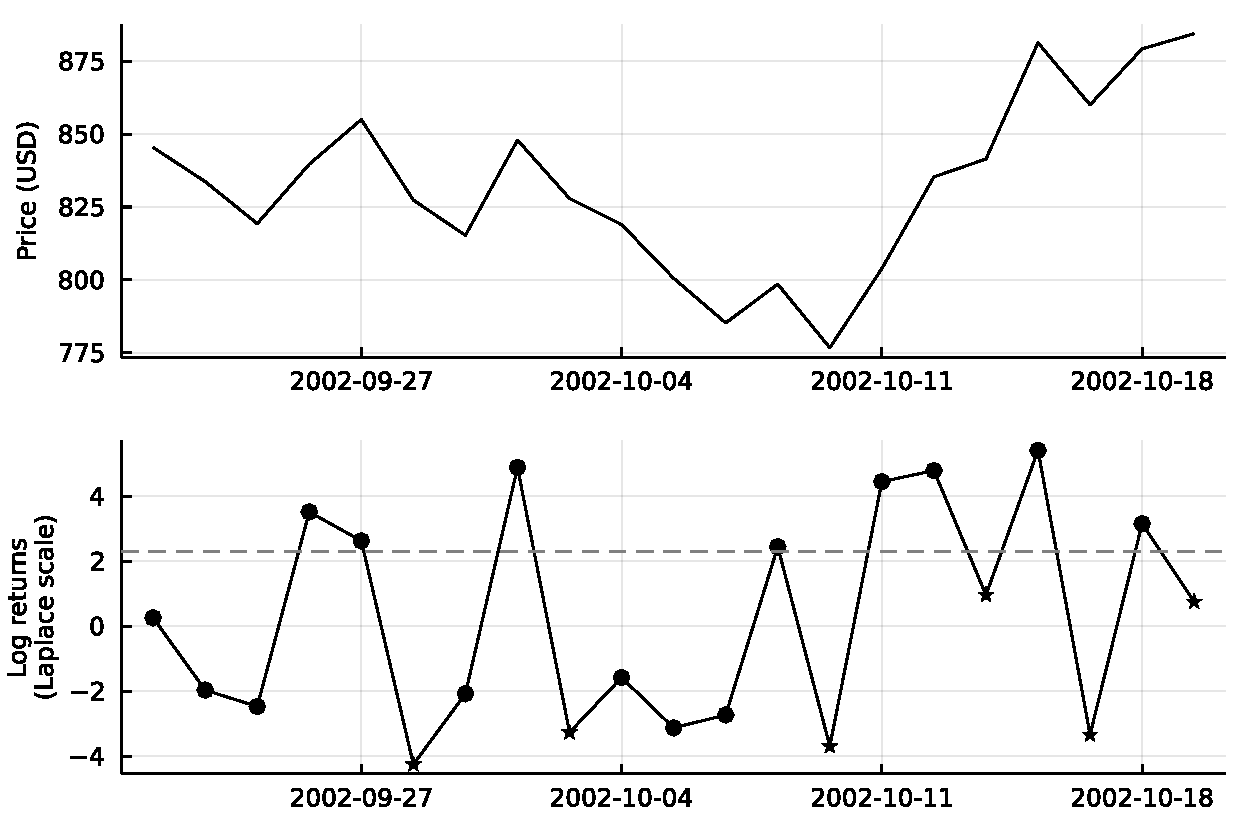
\includegraphics[scale=0.70]{../tail-switching/figures/spy_tail_switch.pdf}
  \caption{S\&P 500 price and log returns on a Laplace scale, during a financially turbulent period in 2002.
  Tail switches across $u=F_{\text{Laplace}}^{-1}(0.95)$ (dashed line) denoted with $\star$.}\label{fig:sap500ts}
\end{figure}

Different aspects of tail switching have been
studied.~\cite{bortot2003extremes} examine in particular not just the
occurrences of tail switches, but tail switches from high extremes to low
extremes (i.e.\ $X_t > u > 0 > u' > X_{t+1}$, where $u'$ is small). This
treatment is useful especially useful for finance, where such switches are
common. Tail switching has also been explored in a multivariate setting,
with multivariate Student-$t$ models by~\cite{bernardi2013multivariate}.

Crucially, conditional extreme value models can be applied to time series to
characterize how they tail switch.
The $K=1$ case has previously been studied in the context of time series~\citep{auldphdthesis},
and the $K>1$ case has been studied in an environmental setting~\citep{tendijck2021modeling},
but it is believed that an application of the $K>1$ case in a time series context is novel.
A model can be fit using~\eqref{eq:ht_mix_final} by constructing a dataset $\D' =
\{(X_{t}, X_{t+1})\}_{t=1}^n$, and then fitting on $\D = \{(x,y) \in \D' | x > u\}$ for some large $u>0$.
It is assumed that $\{X_t\}$ is stationary, so that observations in $\D$ are (perhaps approximately) drawn i.i.d.. This assumption is an important ingredient so that model assumptions are met when fitting~\eqref{eq:ht_mix_final}.

\clearpage

\chapter{Methods and results}\label{sec:methods}
We seek to investigate CEVMMs in the
context of time series. In order to assess their efficacy, we begin by testing
them on simulated data. We focus on data simulated from an asymmetric logistic
distribution. The theoretical relevance of the asymmetric
logistic distribution is that it is a multivariate extreme value distribution
(in the sense that it the satisfies the conditions in
Theorem~\ref{thm:mvextypes}). There are several further reasons for choosing
this distribution: it permits several parameters, $\theta$ and $v$, allowing it
to flexibly model a large range of possible
copula~\citep{coles1991modelling}; it is workable analytically since its
conditional distributions are known, and asymptotic properties relevant for our
purposes have already been found.

By simulating asymmetric logistic data, we show the details of how to fit CEVMM
models; consider the logistic distribution as an alternative marginal
distribution; propose a method for regularizing the mixture likelihoods, and
illustrate methods for quantifying uncertainty in CEVMM models with the
moving block bootstrap.

Finally we use the methods and algorithms developed
on the asymmetric logistic data to apply CEVMMs
to UK electricity imbalance price data.
Imbalance prices are seasonal, so we first perform a deseasonalization
prior to model fitting. We show that there is an extremal dependence structure
in the deseasonalized imbalance price, and demonstrate that
CEVMM models can be useful for managing risk associated with the extremes of
these residuals.

All the code written can be found on GitHub, see \url{https://github.com/lippirk/edi-diss}.

\section{The 3-dimensional asymmetric logistic model}\label{sec:asymlog}

The 3-dimensional asymmetric logistic distribution with Fréchet margins is
defined below via its cumulative distribution function.
\begin{equation}
  \label{eq:3dimasslog}
  \begin{split}
  F(x) &= \exp\left(-V(x)\right),\, x \in \R_{+}^3,\\
V(x) &= \theta_0 x_0^{-1} + \theta_1 x_1^{-1} + \theta_2 x_2^{-1}
     +\theta_{01}\left\{(x_0^{-1/v_{01}} + x_1^{-1/v_{01}})^{v_{01}}\right\}
+\theta_{02}\left\{(x_0^{-1/v_{02}} + x_2^{-1/v_{02}})^{v_{02}}\right\}\\
     &+\theta_{12}\left\{ (x_1^{-1/v_{12}} + x_2^{-1/v_{12}})^{v_{12}}\right\}
+\theta_{012}\left\{(x_0^{-1/v_{012}} + x_1^{-1/v_{012}} + x_2^{-1/v_{012}})^{v_{012}}\right\},\\
\text{subject to  }\;
&\theta_0+\theta_{01}+\theta_{02}+\theta_{012}=1,\,
\theta_1+\theta_{01}+\theta_{12}+\theta_{012}=1,\,
\theta_2+\theta_{01}+\theta_{02}+\theta_{012}=1,\\
&0<v_{01},v_{02},v_{12},v_{012} < 1,\,
0<\theta_0,\theta_1,\theta_2,\theta_{01},\theta_{02},\theta_{12},\theta_{012}.
\end{split}
\end{equation}
When referring to `$\theta$' and `$v$' we mean
$(\theta_0,\theta_1,\theta_2,\theta_{01},\theta_{02},\theta_{12},\theta_{012})$
and $(v_{01}, v_{12}, v_{012})$ respectively. In terms of notation,
we will sometimes write, for example, $\theta_{/012}$ to mean $(\theta_0,\theta_1,\,\ldots,\theta_{12})$,
i.e.\ all the $\theta$'s except $\theta_{012}$.

The equality constraints on
$\theta$ ensure that the marginals of $F$ are unit
Fréchet.
Rather than working directly with~\eqref{eq:3dimasslog}, we use it to
construct an order-2 Markov process~\eqref{eq:3dimasslogmarkovprocess}, given by
\begin{equation}\label{eq:3dimasslogmarkovprocess}
  \begin{split}
  &X_{0} \sim F_{0},\\
  &X_{1}\,|\,X_0=x_0 \sim F_{1|0}(\cdot; x_0),\\
  &X_{t+2}\,|\,X_{t+1}=x_{t+1},\,X_t=x_t \sim F_{2|1,0}(\cdot; x_{t+1}, x_t),\\
\end{split}
\end{equation}
where $F_{1|0}$ and $F_{2|1,0}$ are the conditionals of $F$.
A stationary process can be specified by imposing the constraint
$\prob(X_t \leq x,X_{t+1}\leq y) = \prob(X_{t+1} \leq x,X_{t+2}\leq y),\
\forall x,\,y>0$, which implies $\theta_{01} = \theta_{12} \text{ and } v_{01} =
v_{12}$.

Using inverse sampling, it is possible to draw from
\eqref{eq:3dimasslogmarkovprocess}. Notice how
decreasing the $v$'s and increasing $\theta_{01},\,\theta_{02},\,\theta_{012}$
increases dependence between the r.v.s $X_{t+2}$, $X_{t+1}$ and $X_{t}$.

\clearpage

\subsection{Theoretical Extremal Dependence}

We are interested in particular in the extremal dependence of
$X_0,\,X_1$ and $X_2$. Since we know the conditionals $F_{1|0}$ and
$F_{2|1,0}$ in~\eqref{eq:3dimasslogmarkovprocess}, we can calculate the
dependence directly. However, we also want the normalization constants
necessary for limits such as~\eqref{eq:htassump} to exist, as then we
can compare algorithmic results to what is expected asymptotically.
These results exist already for $F_{1|0}$ and $F_{2|1,0}$, with $X_i$'s in exponential
margins~\citep{papastathopoulos2017extreme,https://doi.org/10.48550/arxiv.1903.04059}.
These are summarised by
\begin{equation}\label{eq:exp_margin_res}
    \begin{split}
      &\prob(X_2 \leq z | X_1 = x) \ra_{x\ra\infty} H_1(z),\\
      &\prob(X_2 \leq z | X_0 = x) \ra_{x\ra\infty} H_2(z),\\
      &\prob(X_2 \leq z | X_0 = x, X_1 = y) \ra_{x\ra\infty,y\ra\infty} H_3(z),\\
      &\prob(X_2 - x \leq z | X_1 = x) \ra_{x\ra\infty} H_4(z),\\
      &\prob(X_2 - x \leq z | X_0 = x) \ra_{x\ra\infty} H_5(z)\text{ and }\\
      &\prob(X_2 +v_{012}\log(\exp(-x/v_{012})+\exp(-y/v_{012}))\leq z | X_0 = x,
      X_1 = y) \ra_{x\ra\infty,y\ra\infty} H_6(z).
    \end{split}
  \end{equation}
The distributions $H_i$ are not particularly important for our purposes --- all
that matters here is that they are
non-degenerate.
For consistency with the results from~\cite{keef2013estimation}, we would ideally work in Laplace margins. Fortunately
the results from~\eqref{eq:exp_margin_res} carry over easily from exponential to Laplace
margins. Note that
\begin{equation}\label{eq:exp_to_lap_res}
    \left(F_{\text{Laplace}}^{-1}\circ F_{\text{exponential}}\right) (x)=
    x - \log 2\text{, whenever $x > \log\,2=F_{\text{exponential}}^{-1}(0.5)$}.\\
  \end{equation}
Equation~\eqref{eq:exp_to_lap_res} implies that the limits associated with $H_1,\ldots,H_6$
in expression~\eqref{eq:exp_margin_res}
also hold in Laplace margins. This allows us to construct a CEVMM that
captures the asymptotic extremal dependence between $X_{t+1}$ and $X_{t}$ with
\begin{equation}\label{eq:asslog_order1}
  \prob\left(X_{t+1}\leq z\middle| X_{t} = x\right) \approx \pi G_1 (z - x) + (1-\pi) G_2\left(z\right)
  \text{ for large }x.
\end{equation}
We can also construct a CEVMM for the capturing the asymptotic extremal dependence between
$X_{t},X_{t+1}$ and $X_{t+2}$ with
\begin{equation}\label{eq:asslog_order2}
  \begin{split}
    \prob\left(X_{t+2}\leq z\middle| X_{t} = x, X_{t+1}=y\right) &\approx
  \pi_{1} G_1 (z) + \pi_{2} G_2\left(z\right) + \pi_{3}G_3\left(z\right)
  +\pi_4 G_4(z - y)
  + \pi_5 G_5(z - x)\\
    &+ \pi_6 G_6(z + v_{012}\log[\exp(-x/v_{012})+\exp(-y/v_{012})]),
\end{split}
\end{equation}
where $(\pi_{1},\,\ldots,\,\pi_6)\in\mathcal{S}_6$, and at least one of $x$ or $y$
is large.
The $G_k$'s in~\eqref{eq:asslog_order2} correspond to the $H_k$'s in~\eqref{eq:exp_margin_res}.
In general the mixture probabilities $\pi_k$ may depend on $x$ and $y$.
For example, if both $x$ and $y$ are very large, then we ought to have $\pi_3,\pi_6$
non zero, with the other mixtures negligible.
\begin{figure}[htp]
  \centering
  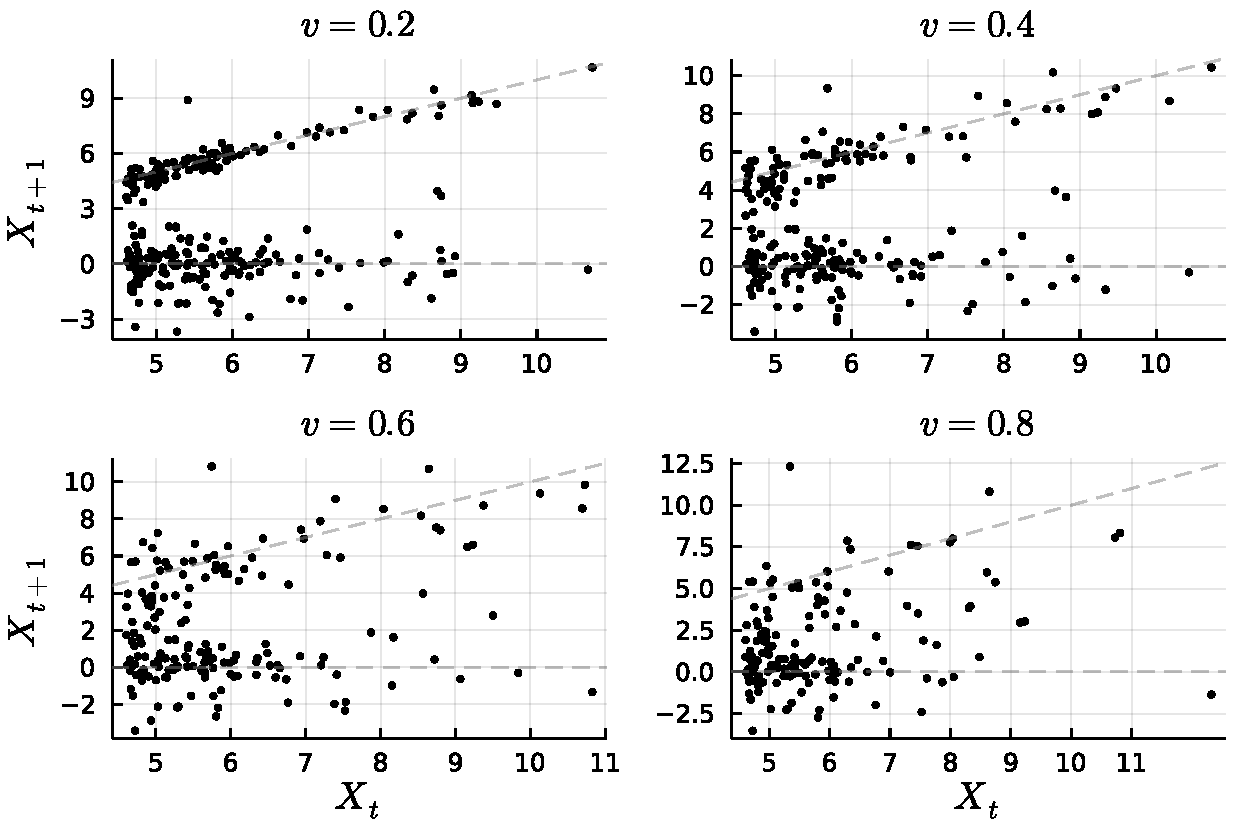
\includegraphics[scale=0.75]{../asym-log/figures/3dim-x2-vs-x1-laplace-scale.pdf}
  \caption{$X_{t+1}$ vs. $X_{t}$, on unit Laplace scale, for
    $\theta_{/012}=0.3$ and
    different values of $v$ (using the same random
seed). The theoretical modes are shown in grey.}\label{fig:asslogx2vsx1} \end{figure}
Figure~\ref{fig:asslogx2vsx1} depicts realizations of $X_{t+1}$ and $X_{t}$,
conditional on $X_{t}$ large. Adopting notation from~\cite{keef2013estimation} for the
normalization functions ($a_k(x) = x^{\beta_k}$, $b_k(x) = \alpha_k x$) they
are characterized by $(\alpha_1,\beta_1)=(1,0)$ and $(\alpha_2,\beta_2)=(0,0)$,
and so we see straight lines. We will fit CEVMMs on this data. Notice that
variance around the modes increases with $v$. This is due to $v$ acting as a
dependence parameter (high $v$ meaning low dependence and vice versa). It
follows that fitting CEVMMs will be easier to fit when relevant variables have
high dependence, and at the opposite extreme, CEVMMs will not be a sensible
model if $v$ is close to 1, since in the $v=1$ case the variables are
independent.

\clearpage
\subsection{Fitting conditional extreme value mixture models --- a worked example}\label{sec:worked_example}

We begin with a worked example of how to fit CEVMMs
to asymmetric logistic data.
First, we generate data from~\eqref{eq:3dimasslogmarkovprocess}. To avoid
the need to generate copious amounts of data, we produce 100 independent
realizations of the Markov process, each of length 30, crucially conditioning on $X_{0} > q
= F_{\text{Fréchet}}^{-1}(0.99)$ for each of the 100 chains to ensure
several extreme values. Let $X^j$ be the $j$th chain, then we form the datasets
$\D' = \{(X^j_{t},X_{t+1}^j) | j=1,\ldots,100, t=0,\ldots,28\}$,
and $\D = \{(x,y)\in \D' | x > u\}$, where $u=3\approx F_{\text{Laplace}}^{-1}(0.975)$.
The size of $\D$ is 460. Figure~\ref{fig:worked_example_data} shows the data generated, with $\D'$ on the
left and $\D$ on the right. The parameters used were
$\theta_0=\theta_1=\theta_2=0.1$, $\theta_{01}=\theta_{02}=\theta_{012}=0.3$
and $v_{01}=v_{02}=v_{012}=0.5$.
\begin{figure}[htp]
  \centering
  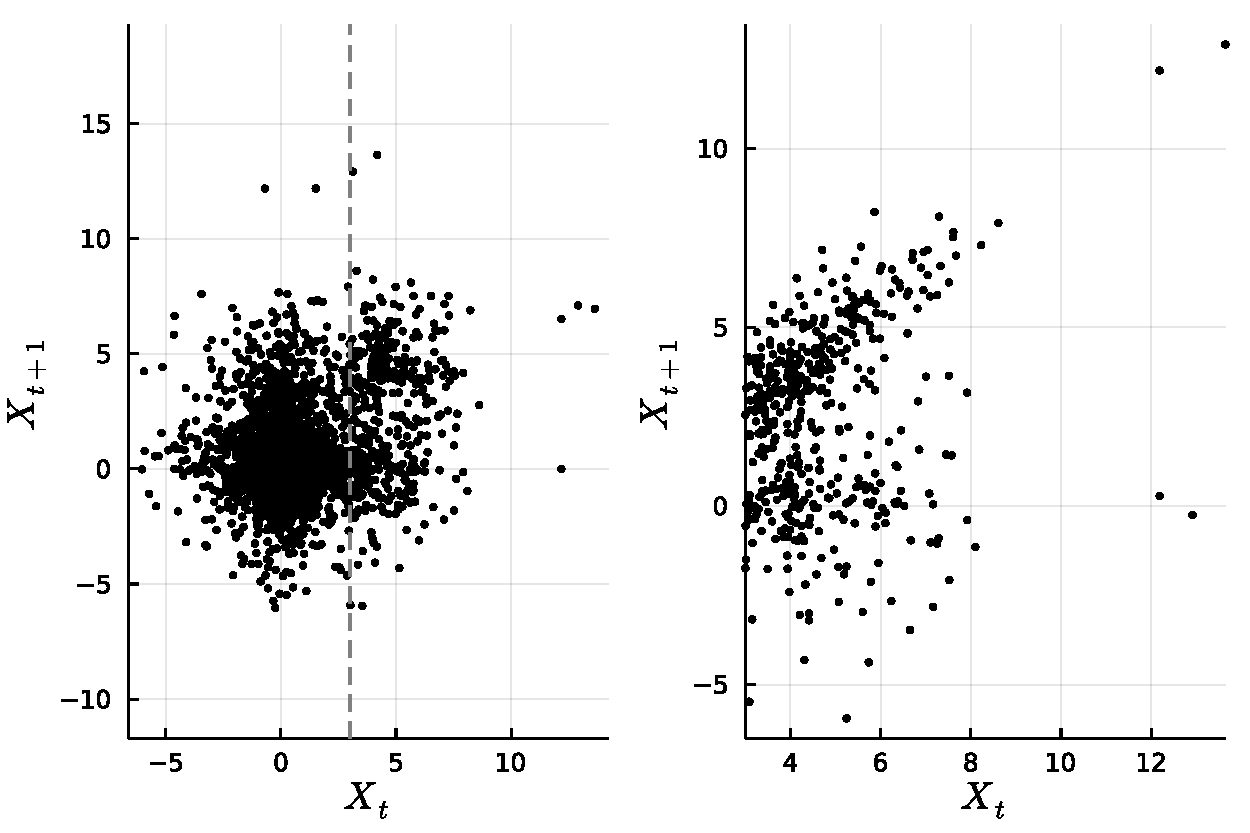
\includegraphics[scale=0.7]{../ht-em/figures/worked_example_data.pdf}
  \caption{Data used for the worked example, in Laplace margins. The threshold
    $u$ is shown as a dashed grey line on the left plot.
}\label{fig:worked_example_data}
\end{figure}

For fitting, we use the normal approximations as
in~\eqref{eq:ht_mix_fitting_step}, and pretend that the normalizing
functions are unknown. The latter is both pedagogical and important if we wish
to fit these models to general data. In other words, we are fitting
$\theta=(\pi,\alpha_1,\alpha_2,\beta_1,\beta_2,\mu_1,\mu_2,\sigma_1,\sigma_2)$
in the model
\[
  \prob\left(X_{t+1}\leq z\middle| X_{t} = x\right)
  =  \pi \Phi\left(\frac{z - \alpha_1 x}{x^{\beta_1}};\mu_1,\sigma_1^2\right)
  +  (1-\pi) \Phi\left(\frac{z - \alpha_2 x}{x^{\beta_2}};\mu_2,\sigma_2^2\right).
\]
Note that we are making an assumption that each data point is i.i.d..
We use the EM algorithm~\ref{appendix:htnormalem} to fit the parameters in this model. The parameter space is slightly awkward because of the constraints
\begin{equation}\label{eq:constraints_k_2}
  0 \leq \pi \leq 1,\, -1 \leq \alpha_1\leq\alpha_1 \leq 1,\,
  0 \leq \beta_1,\beta_2 \leq 1,\, 0 < \sigma_1,\sigma_2.
\end{equation}
The reason for constraints on $\pi$ and $\sigma$ should be clear.
The bounds on the $\alpha$'s and $\beta$'s are from~\cite{keef2013estimation},
but we impose $\alpha_1\geq\alpha_2$ to ensure identifiability as in~\cite{tendijck2021modeling}.
Numerically it is helpful to perform parameter transformations to allow
us to work over $\reals^9$, unconstrained. The following transformations
are proposed,
\begin{equation}\label{eq:htconstr}
  \begin{split}
  \pi_k' &= \text{logit}(\pi_k),\,\pi_k = \text{sigmoid}(\pi_k'),\\
  \beta_k' &= \text{logit}(\beta_k),\,\beta_k = \text{sigmoid}(\beta_k'),\\
  \sigma_k' &= \log(\sigma_k),\,\sigma_k = \exp(\sigma_k'),\\
  \alpha_1' &= \text{logit}\left(\frac{\alpha_1 + 1}{2}\right),\,\alpha_1 = 2\text{sigmoid}(\alpha_1') - 1,\\
  \alpha_2' &= \text{logit}\left(\frac{\alpha_2 + 1}{\alpha_1 + 1}\right),\,
  \alpha_2 = (\alpha_1 + 1)\text{sigmoid}(\alpha_2') - 1.\\
\end{split}
\end{equation}
In the transformed space, we take advantage of
an implementation of the L-BFGS algorithm from~\cite{mogensen2018optim}, which
allows for fast model fitting.

We fit several models with EM using different (random) initial values
for $\theta$. Some results are shown in
Table~\ref{table:ht_worked_example_results_1} (omitting the $\mu$ and $\sigma$
values).
We see that the initial value of $\theta$ greatly affects the fitting of $\alpha$ and $\beta$ ---
this is likely because we are optimizing over a highly multimodal landscape.
According to theory, we are expecting $(\alpha_1,\,\alpha_2,\,\beta_1,\,\beta_2) = (1,0,0,0)$.
We see some poor fits (e.g.\ seed 1), but thankfully the estimates
with the highest likelihood are close to the expected values.
\begin{table}[htp]\centering
  \begin{tabular}{c |c |c |c |c |c |c}
Seed & $\hat\pi$ & $\hat\alpha_1$ & $\hat\alpha_2$ & $\hat\beta_1$ & $\hat\beta_2$ & Log Likelihood \\
    \hline
  1 & 0.48 & 1.00 & -1.00 & 0.89 & 0.95 & -1002.45 \\
  2 & 0.51 & 0.93 & -0.08 & 0.00 & 0.14 & -985.77 \\
  3 & 0.03 & 1.00 & -1.00 & 0.00 & 0.93 & -1056.30 \\
  4 & 0.49 & -0.12 & -1.00 & 0.02 & 0.94 & -995.32 \\
  5 & 0.49 & -0.10 & -0.10 & 0.00 & 0.89 & -994.66 \\
  6 & 0.51 & 0.93 & -0.08 & 0.00 & 0.14 & -985.77 \\
  7 & 0.47 & 1.00 & 1.00 & 0.88 & 1.00 & -1003.74 \\
  8 & 0.49 & -0.12 & -1.00 & 0.02 & 0.94 & -995.32 \\
  9 & 0.51 & 0.93 & -0.08 & 0.00 & 0.14 & -985.77 \\
  10 & 0.51 & 1.00 & -0.07 & 0.00 & 0.00 & -987.19 \\
\end{tabular}
 \caption{Parameter estimates
  and log-likelihoods, to 2 decimal places, obtained when fitting CEVMMs
to asymmetric logistic data, with starting values initialized using different
random seeds.\label{table:ht_worked_example_results_1} }
\end{table}

We continue our analysis with the parameters that induce the highest
likelihood, i.e.\ seed 2 (though seeds 2, 6 and 9 yield equivalent results).
We can examine the fit visually in Figures~\ref{fig:worked_example_contour_1} and
\ref{fig:worked_example_vs_true_1}. Figure~\ref{fig:worked_example_contour_1}
shows the data used to fit the model, colour coded according to which mixture is
more likely. Contours of the fitted normal mixture model are shown conditional on the value of $X_t$,
such that taking a vertical cross-section yields a probability density.
Figure~\ref{fig:worked_example_vs_true_1} shows four of these cross sections,
along with their expected probability densities. Here the expected density
is calculated using $F_{1|0}$, by taking the appropriate partial derivative
(using the chain rule to account for the change to Laplace margins).
The model seems to have captured the mode corresponding to $\alpha=1$ quite well,
but performs poorly at the mode corresponding to $\alpha=0$. One reason for
this is that it is impossible for a normal distribution to properly approximate
the discontinuity in the gradient of the true conditional density at $0$.
\begin{figure}[htp]
  \centering
  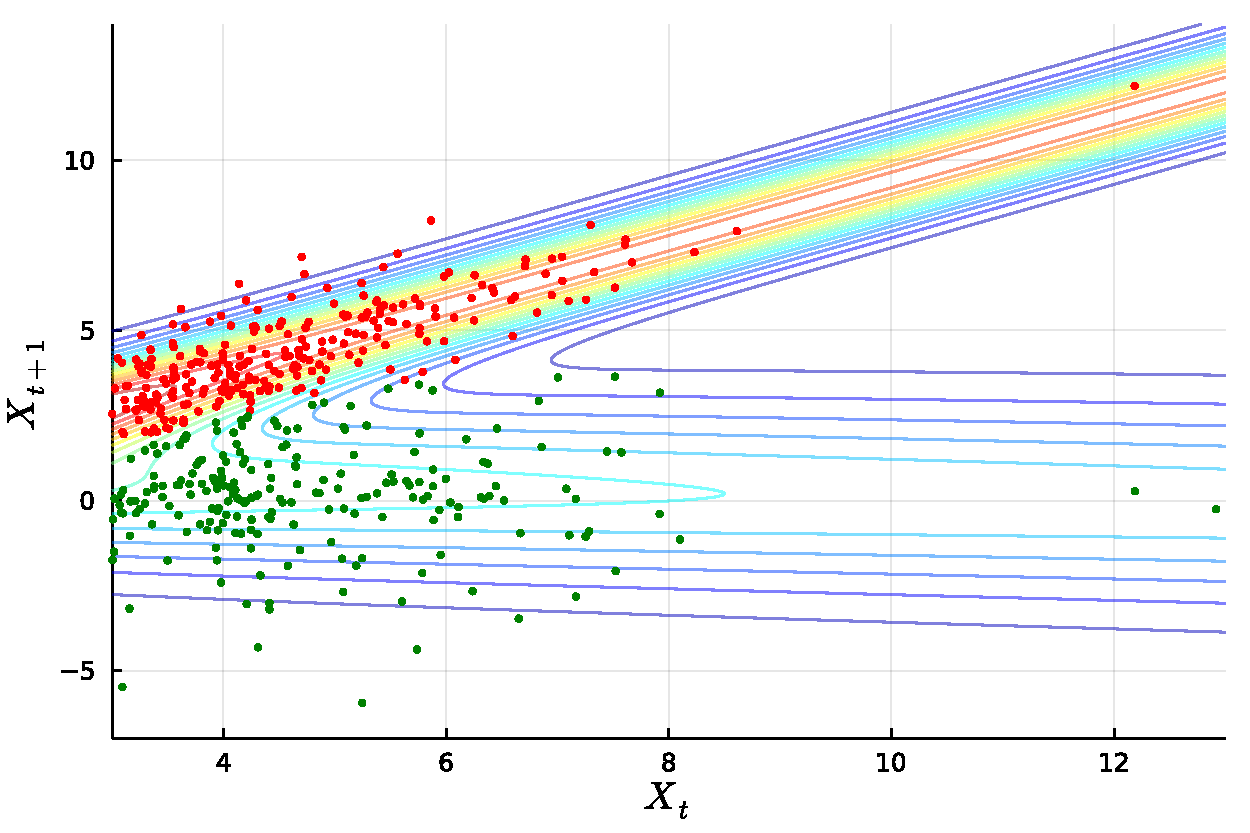
\includegraphics[scale=0.7]{../ht-em/figures/worked_example_contour_fit.pdf}
  \caption{$X_{t+1}$ vs. $X_t$, with each data point colour coded according to
    its more likely mode (a.k.a\ mixture component). The coloured
    lines show contours of the modelled normal mixture density
    for $X_{t+1}\,|\,X_{t}$, when viewed as a function of both $X_{t+1}$ and $X_{t}$.
}\label{fig:worked_example_contour_1}
\end{figure}
\begin{figure}[htp]
  \centering
  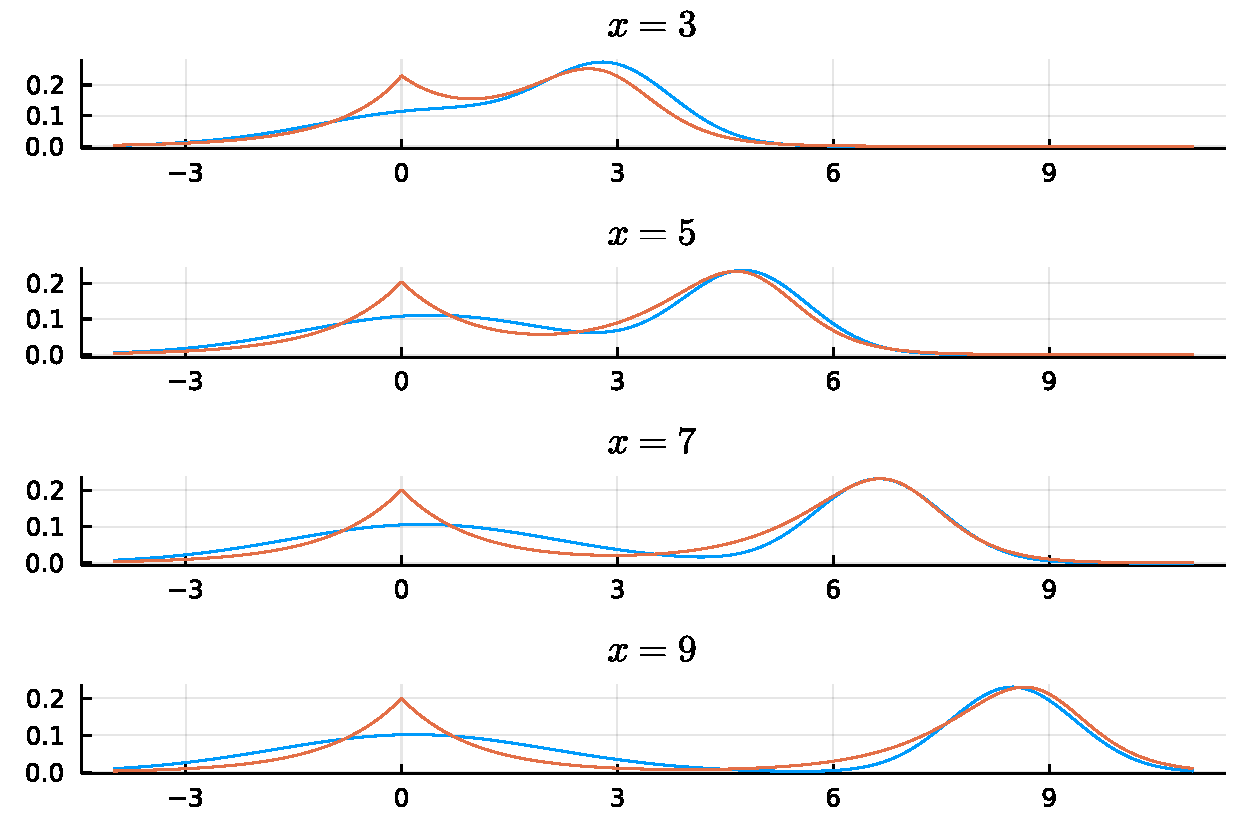
\includegraphics[scale=0.7]{../ht-em/figures/worked_example_vs_true.pdf}
  \caption{Probability densities of $X_{t+1}|X_{t}=x$ for 4 fixed values of $x$.
    The expected densities are shown in orange, and fitted densities in blue.
    These plots can be thought of as vertical cross sections of Figure~\ref{fig:worked_example_contour_1} at
    $X_t=x$.
   }\label{fig:worked_example_vs_true_1}
\end{figure}
\begin{figure}[htp]
  \centering
  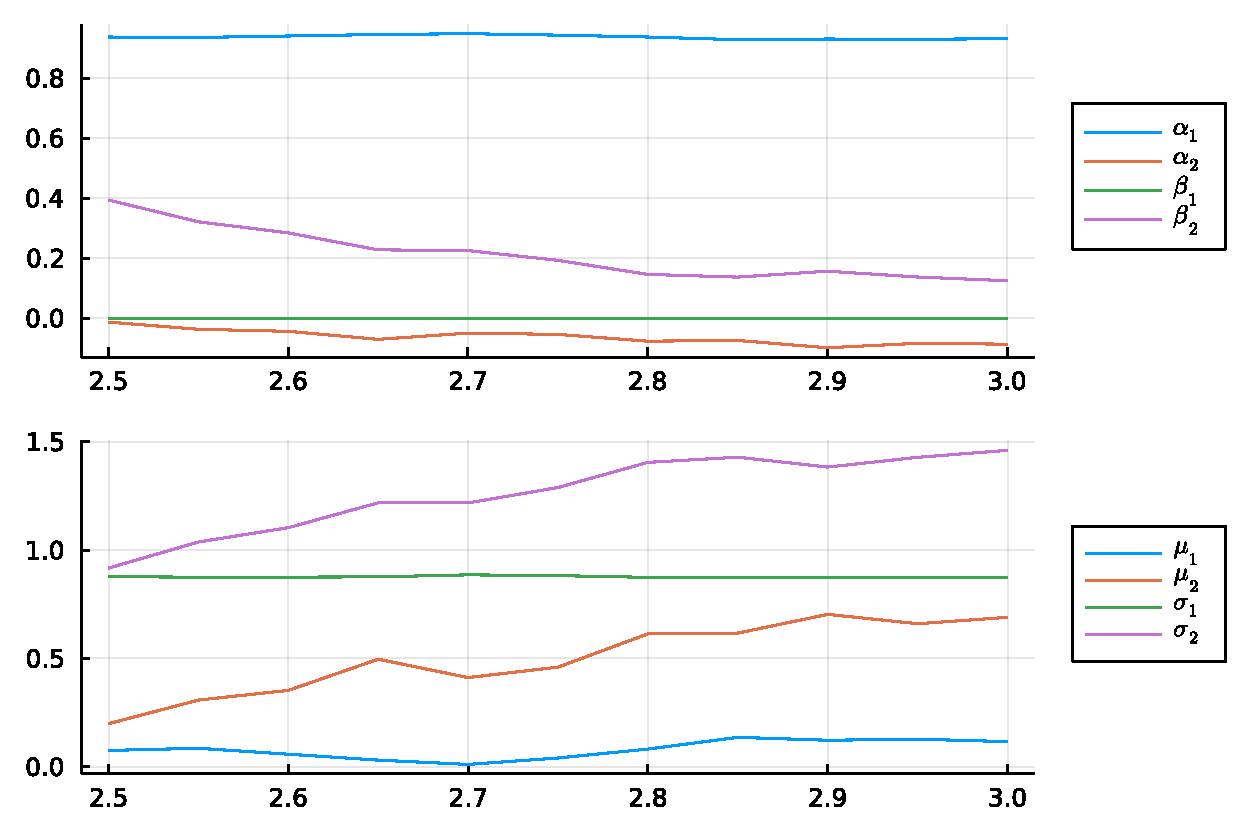
\includegraphics[scale=0.7]{../ht-em/figures/worked_example_check_u.pdf}
  \caption{Effect of decreasing $u$ (down from $u=3$) on the fitted parameters.}\label{fig:worked_example_1_check_u}
\end{figure}
\begin{figure}[htp]
  \centering
  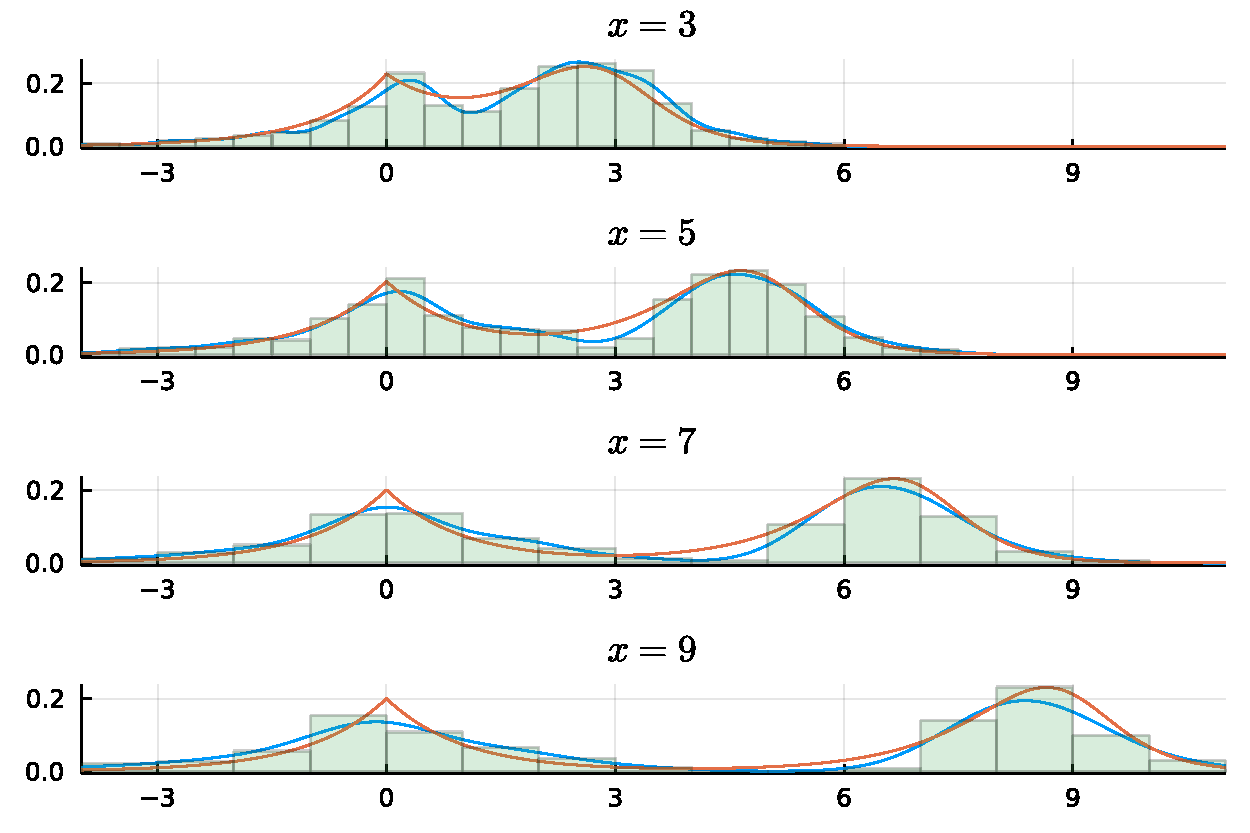
\includegraphics[scale=0.7]{../ht-em/figures/worked_example_vs_true_ecdf.pdf}
  \caption{Probability densities of $X_{t+1}|X_{t}=x$ for fixed values of $x$ (Laplace margins).
    Expected densities are shown in orange. 10000 samples were drawn from the
    estimated distribution function; the associated Gaussian kernel density estimators
    for these samples are shown in blue, with histograms of the samples in green.
   }\label{fig:worked_example_vs_true_1_resids}
\end{figure}
\FloatBarrier
It is expedient to reduce $u$ as much as
possible to reduce the variance of the ECDF estimators. This can be achieved by
reducing $u$ until the parameters
$(\alpha_1,\alpha_2,\beta_1,\beta_2,\mu_1,\mu_2,\sigma_1,\sigma_2)$ begin to
change~\citep{tendijck2021modeling}.
With the aid of Figure~\ref{fig:worked_example_1_check_u}, which
shows the effect of $u$ on the fitted parameters, we choose $u=2.9$.
The rationale here is that both $\beta_2$, $\sigma_2$ and $\mu_2$ begin to change
for $u$ below $2.9$.

Finally, we sample residuals (this is explained in Appendix~\ref{appendix:nonparametriccevmm},
here we sample each classification $M=500$ times)
to obtain the semi-parametric model in the form~\eqref{eq:ht_mix_final}.
Comparing the semi-parametric model fit
(Figure~\ref{fig:worked_example_vs_true_1_resids}) to the fit of the model with
normal assumptions (Figure~\ref{fig:worked_example_vs_true_1}), we see that
moving to use residuals has somewhat remedied the issue of poor fit at the
lower mode, since an ECDF function is more easily able to capture the
discontinuity in the gradient of the expected density. There is, however, still a
bias, perhaps induced by the fact that the theoretical values for $\alpha$ and
$\beta$ were not obtained exactly during the fitting process.

From the above, there are a few things that should be taken into account when
fitting these models. The EM algorithm is sensitive to initial values. Here we
fit several models, and selected the one with the highest likelihood, but in
general this may lead to overfitting. Sensitivity may be further exacerbated if
we tried to model $K \geq 3$ modes. We work around this issue
practically later when establishing uncertainty by adding regularization
(see Section~\ref{sec:regularization}).
Also, the best fitted model in terms of log-likelihood found biased values for
the normalizing function constants, which possibly induces the slight bias in
the modes we see in Figure~\ref{fig:worked_example_vs_true_1_resids}. It is
unclear exactly the cause of this bias, but potential reasons include an
insufficiently large threshold or overfitting.

Overall, we can expect the EM algorithm to perform a reasonable fit,
since $(\hat\alpha_1,\hat\beta_1)=(0.93,-0.08)$ and
$(\hat\alpha_2,\hat\beta_2)=(0.00,0.14)$  are reasonably close to the
true values.

\FloatBarrier
\subsection{A look at  logistic margins}

The cause of this undesirable `kink' in the true conditional density
in Figure~\ref{fig:worked_example_vs_true_1} is
due to definition of the Laplace density. The logistic distribution has
similar asymptotic properties to the Laplace distribution in the upper and lower tails (both tails are symmetric and are exponential).
In particular, the
results from~\eqref{eq:exp_to_lap_res} hold in logistic margins.
Crucially, however, the logistic density is smooth, meaning that the conditionals
are more likely to be easily modelled by a mixture of Gaussians. Repeating the above with the same
data, but with logistic margins and starting with $u=3.65\approx
F_{\text{logistic}}^{-1}(0.975)$ (for fair comparison), yields
similar parameter estimates $(\hat\alpha_1,\,\hat\alpha_2,\,\hat\beta_1,\,\hat\beta_2)=(0.93,\,-0.08,\,0.00,\,0.17)$, but more convincing looking
normal mixture densities (see Figure~\ref{fig:worked_example_logistic_vs_true}),
especially at the lower mode. However, it is not clear whether moving to logistic
margins actually improves the semi-parametric model, since Figures~\ref{fig:worked_example_logistic_vs_true_resids} and~\ref{fig:worked_example_vs_true_1_resids} are very similar. Notice that the logistic version suffers from the same bias problem as the Laplace version.
\begin{figure}[htp]
  \centering
  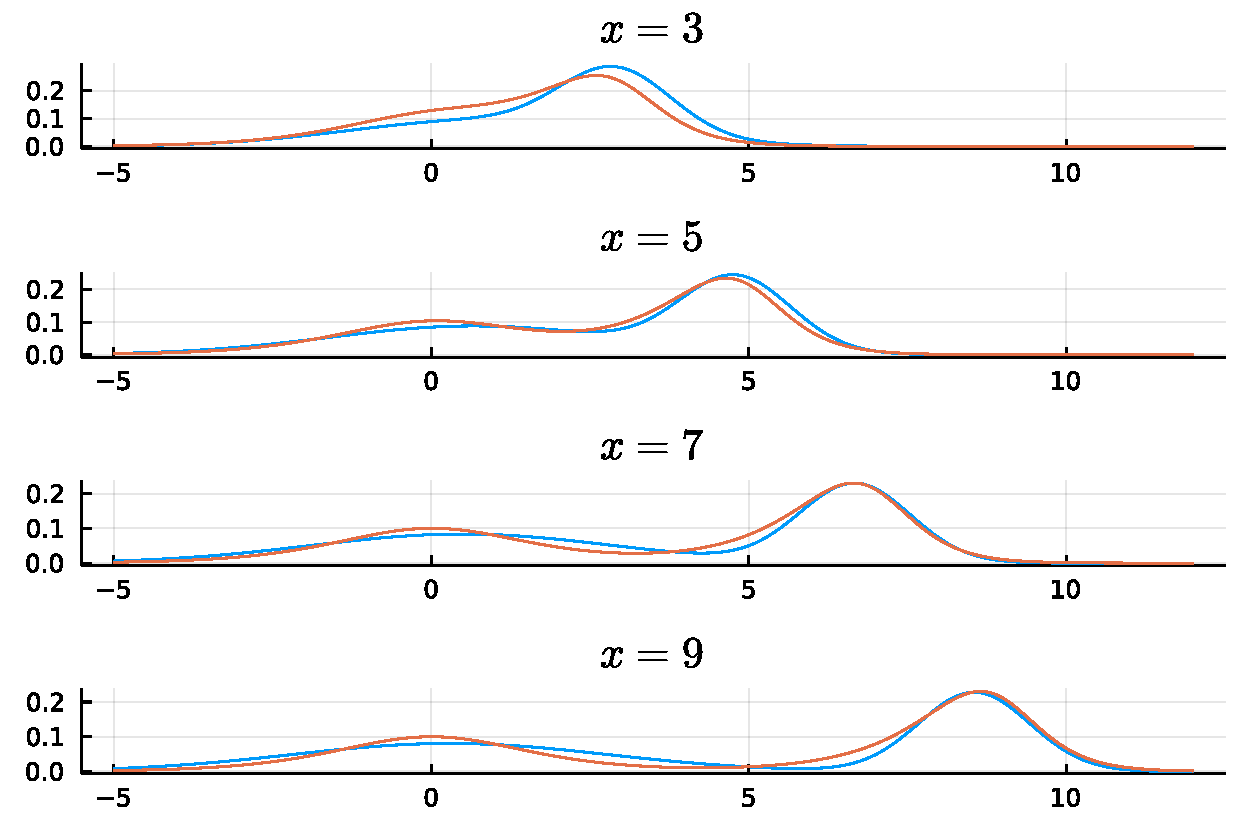
\includegraphics[scale=0.7]{../ht-em/figures/worked_example_logistic_vs_true.pdf}
  \caption{Probability densities of $X_{t+1}|X_{t}=x$ for fixed values of $x$ (logistic margins).
    True densities are shown in orange, and fitted densities in blue.
   }\label{fig:worked_example_logistic_vs_true}
\end{figure}
\begin{figure}[htp]
  \centering
  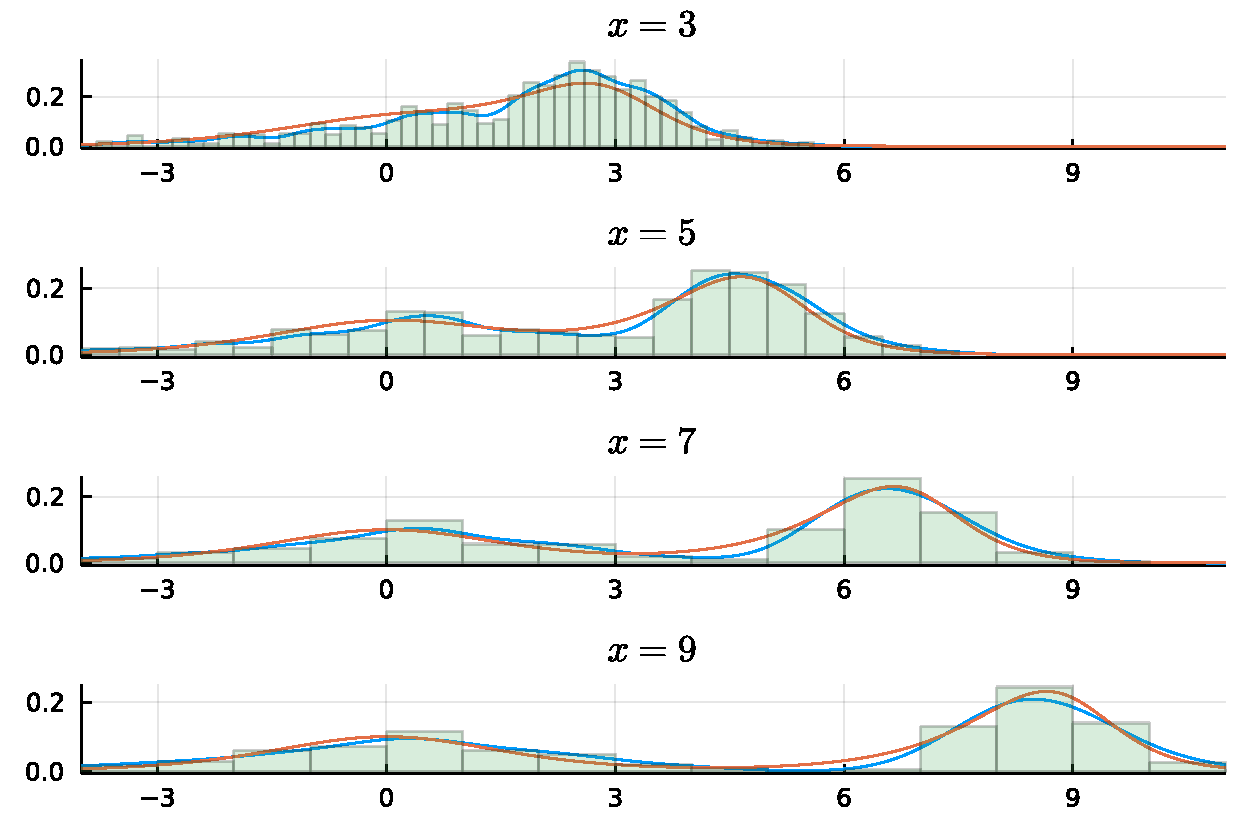
\includegraphics[scale=0.7]{../ht-em/figures/worked_example_logistic_vs_true_resids.pdf
}
  \caption{Probability densities of $X_{t+1}|X_{t}=x$ for fixed values of $x$ (logistic margins).
    True densities are shown in orange. 10000 samples were drawn from the
    estimated distribution function; the associated Gaussian kernel density estimators
    for these samples are shown in blue, with histograms of the samples in green.
   }\label{fig:worked_example_logistic_vs_true_resids}
\end{figure}

\FloatBarrier
\clearpage
\subsubsection{Simulation study to compare Laplace and logistic margins}\label{sec:lap_vs_log}

To quantitatively examine the effect of the choice of marginal distribution
on the estimated conditional $\hat F_{1|0}$, we perform a simulation study
comparing Laplace and logistic margins. Specifically we generate 100 datasets (each)
for different combinations of $u$, $v$ and $\theta$, fitting CEVMMs and
recording integrated absolute and square errors
with respect to the expected distribution. Mean errors (as well as their standard errors) can then be calculated
by averaging over the 100 datasets. Formulae for these metrics are  given by
\begin{equation}\label{eq:miseandmiae}
  \begin{split}
    \text{MISE}_{x_0}&=\frac{1}{100}\sum_{d=1}^{100}\int_\reals \left(F_{1|0}(x;x_0) - \hat F_{1|0}^{(d)}(x;x_0)\right)^2\md x,\\\text{MIAE}_{x_0}&=\frac{1}{100}\sum_{d=1}^{100}\int_\reals \left|F_{1|0}(x;x_0) - \hat F_{1|0}^{(d)}(x;x_0)\right|\md x,
\end{split}
\end{equation}
where $\hat F^{(d)}_{1|0}$ is the estimated conditional distribution on the $d$th dataset (out of 100),
and the quantities $\text{MISE}_{x_0}$ and $\text{MIAE}_{x_0}$ also implicitly depend on $v$, $u$ and $\theta$.
By varying $x_0$ in~\eqref{eq:miseandmiae}, we test the estimators' efficacy
conditional on different values.
Varying the parameters $v$ and $\theta$, allows us to test across
different types of datasets.
We vary the level of dependence in the data (high, medium and low via $v$: $v=0.3$; $v=0.5$; $v=0.7$,
and low and high via $\theta$: $\theta_{\{0\},\{1\},\{2\}}=0.1,\theta_{/\{0\},\{1\},\{2\}}=0.3$; $\theta_{/012}=0.3$),
and also the threshold for computing the dataset $\D$ via $u=F_0^{-1}(q_u)$.
All models were fit using the same initial parameter estimates.
A subset of the mean integrated square error results, with
low dependence via $\theta$, are shown in
Table~\ref{table:lap_vs_log_table1}.
\begin{table}[htp]
  \centering
  \scalebox{1.0}{
  \begin{tabular}{p{18mm}|p{15mm}|p{20mm}|p{20mm}|p{20mm}|p{22mm}|p{22mm}}
  $(v,q_u)$ & Marginal & $100\text{MISE}_{0.97}$ & $100\text{MISE}_{0.98}$& $100\text{MISE}_{0.99}$& $100\text{MISE}_{0.999}$& $100\text{MISE}_{0.9999}$\\\hline(0.3, 0.95) &Laplace \newline Logistic &\textbf{$\mathbf{0.4 \pm 0.2}$} \newline $0.4 \pm 0.2$ & \textbf{$\mathbf{0.4 \pm 0.2}$} \newline $0.4 \pm 0.2$ &$0.4 \pm 0.3$ \newline \textbf{$\mathbf{0.4 \pm 0.2}$} &$0.5 \pm 0.5$ \newline \textbf{$\mathbf{0.4 \pm 0.3}$} &$0.8 \pm 0.9$ \newline \textbf{$\mathbf{0.6 \pm 0.6}$}\\\hline(0.3, 0.98) &Laplace \newline Logistic &\textbf{$\mathbf{0.4 \pm 0.2}$} \newline $0.4 \pm 0.3$ & \textbf{$\mathbf{0.4 \pm 0.3}$} \newline $0.4 \pm 0.3$ &$0.4 \pm 0.4$ \newline \textbf{$\mathbf{0.4 \pm 0.3}$} &$0.6 \pm 0.7$ \newline \textbf{$\mathbf{0.5 \pm 0.6}$} &$1.0 \pm 1.1$ \newline \textbf{$\mathbf{0.8 \pm 1.1}$}\\\hline(0.5, 0.95) &Laplace \newline Logistic &\textbf{$\mathbf{0.7 \pm 0.4}$} \newline $1.1 \pm 0.7$ & \textbf{$\mathbf{1.0 \pm 0.5}$} \newline $1.5 \pm 1.0$ &\textbf{$\mathbf{1.7 \pm 0.9}$} \newline $2.4 \pm 1.8$ &\textbf{$\mathbf{4.7 \pm 2.9}$} \newline $5.8 \pm 5.2$ &\textbf{$\mathbf{8.1 \pm 5.5}$} \newline $9.7 \pm 9.1$\\\hline(0.5, 0.98) &Laplace \newline Logistic &\textbf{$\mathbf{0.7 \pm 0.3}$} \newline $1.1 \pm 0.6$ & \textbf{$\mathbf{1.1 \pm 0.4}$} \newline $1.6 \pm 0.9$ &\textbf{$\mathbf{1.9 \pm 0.9}$} \newline $2.7 \pm 1.7$ &\textbf{$\mathbf{5.5 \pm 3.2}$} \newline $6.9 \pm 5.1$ &\textbf{$\mathbf{9.6 \pm 6.2}$} \newline $11.7 \pm 9.0$\\\hline(0.7, 0.95) &Laplace \newline Logistic &\textbf{$\mathbf{0.4 \pm 0.3}$} \newline $0.9 \pm 0.4$ & \textbf{$\mathbf{0.6 \pm 0.4}$} \newline $1.6 \pm 0.6$ &\textbf{$\mathbf{1.1 \pm 0.6}$} \newline $3.0 \pm 1.1$ &\textbf{$\mathbf{4.0 \pm 2.3}$} \newline $11.1 \pm 4.0$ &\textbf{$\mathbf{9.2 \pm 5.4}$} \newline $22.5 \pm 8.3$\\\hline(0.7, 0.98) &Laplace \newline Logistic &\textbf{$\mathbf{0.4 \pm 0.2}$} \newline $0.9 \pm 0.3$ & \textbf{$\mathbf{0.6 \pm 0.3}$} \newline $1.5 \pm 0.5$ &\textbf{$\mathbf{1.1 \pm 0.6}$} \newline $2.9 \pm 1.1$ &\textbf{$\mathbf{4.5 \pm 2.8}$} \newline $10.9 \pm 4.3$ &\textbf{$\mathbf{10.4 \pm 6.4}$} \newline $22.4 \pm 8.8$\\\hline
\end{tabular}}\caption{Mean integrated square errors $\pm$ 1 s.d.\ for Laplace and logistic marginals, and for different
parameter combinations. MISEs are multiplied by 100 for readability.\label{table:lap_vs_log_table1}}
\end{table}

The result with the better MISE (Laplace
vs.\ logistic) for a given $v,q_u = F_0(u)$ is shown in bold. The estimators fit
in Laplace margins appear to perform better than the estimators fit in logistic
margins for lower $x_0$, but the performance gap decreases for larger $x_0$.
The logistic margin's improvement for higher $x_0$ may be due to the fact that the
exponential tail approximation improves for larger $x_0$.
The MIAE results yield similar conclusions.

Overall, Laplace margins perform better. They have better mean errors (MISE and MIAE) $82.5\%$ of the time
(averaged over all variables).

\subsection{Regularization}\label{sec:regularization}

Changing initial parameter estimates can drastically affect the resulting model
fit of a CEVMM (e.g.\ see Table~\ref{table:ht_worked_example_results_1}).
This is expected if initial parameter estimates are far from the true values,
but we want to avoid this instability otherwise. We may also
encounter instability when fitting if the data changes slightly, which is
in effect what we do in Section~\ref{sec:cevvm_uncertainty} when bootstrapping
new datasets from an existing one. Regularization is the proposed solution
to avoid such instability.
It is possible to regularize any and every parameter in a model, but it was
found by experimentation on asymmetric logistic datasets that regularization in
the $\sigma$ parameters is sufficient to allow for stable model fitting.
Without this, at least in the $K=2$ case, the fitting
algorithm sometimes has a tendency to either remove one of the mixture components (by sending
$\pi_1$ or $\pi_2$ to zero, and making the corresponding variance large), or
alternatively to assign a very small variance to one of the modes. Neither of
these are desirable when we specifically want 2 mixtures. As such the following
adjusted log-likelihood is proposed,
\begin{align*}
  l_\text{regularized}(\theta) = l(\theta) - \gamma \sum_{k=1}^K (\sigma_k^{-2} + \sigma_k^2 / C),\ \gamma > 0,\, C > 0,
\end{align*}
with the $\sigma_k^{-2}$ term designed to discourage small variances, and the $\sigma_k^2/C$
term to discourage variances from becoming too large. In our implementation,
we fixed $C=20$.

We also generally preferred $\gamma=0.05$, motivated
by a quick experiment. Three datasets were
generated, similar to the one described in Section~\ref{sec:worked_example}, but each has a
different level of dependence ($v=0.3$, $v=0.5$ or $v=0.7$, but
$\theta=(0.1,0.1,0.1,0.3,0.3,0.3)$ held constant throughout).
The threshold was fixed as $u=F_{\text{Laplace}}^{-1}(0.95)$.
CEVMM models were then fit to each dataset, indexed by $v$
for different values of $\gamma\in\{0,0.005,0.05,0.5,5\}$. The results in Table~\ref{table:regularization_3}
show that $\gamma=0.05$ tended to perform better, both in terms of fitted parameters
matching their expected theoretical values, and in terms of log-likelihood (high is better).


\begin{table}[htp]
  \centering
    \begin{tabular}{c |c |c |c |c |c |c |c}
$v$ & $\gamma$ & $\hat{\pi}$ & $\hat{\alpha_1}$ & $\hat{\alpha_2}$ & $\hat{\beta_1}$ & $\hat{\beta_2}$ & Log likelihood \\
    \hline
  0.3 & 0.000 & 0.51 & 1.00 & -1.00 & 0.71 & 0.85 & -1789.00 \\
  0.3 & 0.005 & 0.52 & 0.96 & -1.00 & 0.62 & 0.82 & -1788.52 \\
  0.3 & 0.050 & 0.57 & 1.00 & -0.13 & 0.00 & 0.00 & -1497.89 \\
  0.3 & 0.500 & 0.60 & 1.00 & -0.12 & 0.00 & 0.00 & -1612.62 \\
  0.3 & 5.000 & 0.63 & 1.00 & -0.34 & 0.00 & 0.00 & -1752.90 \\
  0.5 & 0.000 & 0.60 & 1.00 & -1.00 & 0.00 & 0.97 & -1280.03 \\
  0.5 & 0.005 & 0.62 & 1.00 & -0.01 & 0.00 & 0.00 & -1263.10 \\
  0.5 & 0.050 & 0.62 & 1.00 & -0.02 & 0.00 & 0.00 & -1264.42 \\
  0.5 & 0.500 & 0.62 & 1.00 & -0.23 & 0.00 & 0.00 & -1306.99 \\
  0.5 & 5.000 & 0.66 & 1.00 & -0.54 & 0.00 & 0.00 & -1354.92 \\
  0.7 & 0.000 & 0.49 & 1.00 & -1.00 & 0.68 & 0.90 & -831.60 \\
  0.7 & 0.005 & 0.49 & 1.00 & -1.00 & 0.55 & 0.83 & -831.59 \\
  0.7 & 0.050 & 0.47 & 1.00 & -0.16 & 0.00 & 0.00 & -816.93 \\
  0.7 & 0.500 & 0.47 & 1.00 & -0.22 & 0.00 & 0.00 & -820.90 \\
  0.7 & 5.000 & 0.49 & 1.00 & -0.26 & 0.00 & 0.00 & -827.02 \\
\end{tabular}

\caption{Fitted parameters and log-likelihoods for CEVMM fits on the three
datasets described above, for different levels of regularization $\gamma$.\label{table:regularization_3}}
\end{table}


\subsection{Quantifying error in CEVMM models with bootstrapped confidence
intervals}\label{sec:cevvm_uncertainty}

We briefly show that it is possible to produce confidence intervals
for a CEVMM's parameters and its predictions.
Due to the constraints on the parameter space for CEVMMs
(see~\eqref{eq:constraints_k_2} for the constraints in the $K=2$ case),
we cannot construct asymptotic confidence intervals.
The reason for this is that the usual regularity conditions, sufficient for
asymptotic normality of maximum likelihood estimates, do not necessarily hold
--- in particular our estimates may lie on the boundary of the parameter space.
In order to establish confidence intervals for a CEVMM model we must
try to quantify sources of error directly. These sources include
error in the parameter estimates $\theta=(\pi,\alpha,\beta,\mu,\sigma)$;
error due to the choice of threshold $u$ (is $u$ large enough
    for the asymptotic approximation to be valid but small enough such that
    variance of the model parameters is low?), and error due to false assumptions (e.g.\ the i.i.d.\ assumption not being met).

It is possible to estimate uncertainty due to error in the parameter
estimates using the bootstrap~\citep{efron1994introduction}.
It would be difficult to estimate the error due to $u$; it may be possible via
a combination of the bootstrap and varying $u$, but this is likely to be very
computationally intensive, and also it would hard to decouple from
the estimated error in the parameters.
Estimating error due to a false assumption is incredibly difficult,
since if an assumption has been broken it is likely that the model is invalid.

%It may be possible to estimate the uncertainty due to $u$ (by bootstrapping
%datasets and varying $u$, for example) but it would be difficult
%to decouple the effects of (1) from the estimate of the error.

As such, we concentrate on only uncertainty due to the model parameters. From a
high level this means that we run Algorithms~\ref{alg:normalht}
and~\ref{alg:resids} on many bootstrapped datasets to obtain many models. Then
we can construct empirical distributions, and hence confidence intervals, for a
quantity of interest by computing it with each model. Note that there is unfortunately no
guarantee that any resulting empirical distribution will be accurate.
We demonstrate the procedure for
a dataset generated using the asymmetric logistic model.
The dataset $\D_1$ is a single time series of length 15000, generated
using~\eqref{eq:3dimasslogmarkovprocess} having set
$\theta = (0.1,0.1,0.1,0.3,0.3,0.3)$, $v = (0.5,0.5,0.5)$. After moving the time series to Laplace
margins, we set threshold $u = F_{\text{Laplace}}^{-1}(0.95)$. See
Figure~\ref{fig:block_bootstrap_Xs} for a visual representation of the data, and
Table~\ref{table:15000_fit} for the fitted parameters, with regularization $\gamma = 0.05$.

\begin{table}[htp]
  \centering
    \begin{tabular}{c |c |c |c |c |c |c |c |c |c}
$\hat{\pi}$ & $\hat{\alpha_1}$ & $\hat{\alpha_2}$ & $\hat{\beta_1}$ & $\hat{\beta_2}$ & $\hat{\mu_1}$ & $\hat{\mu_2}$ & $\hat{\sigma_1}$ & $\hat{\sigma_2}$ & Log likelihood \\
    \hline
  0.5066 & 1.0000 & 0.0002 & 0.0000 & 0.0000 & -0.5491 & 0.4895 & 1.1040 & 1.4649 & -1410.2723 \\
\end{tabular}

\caption{Fitted parameters and log-likelihood for a CEVMM fit on $\D_1$, with $u=F_{\text{Laplace}}^{-1}(0.95)$, $\gamma = 0.05$.\label{table:15000_fit}}
\end{table}

\begin{figure}[htp]
  \centering
  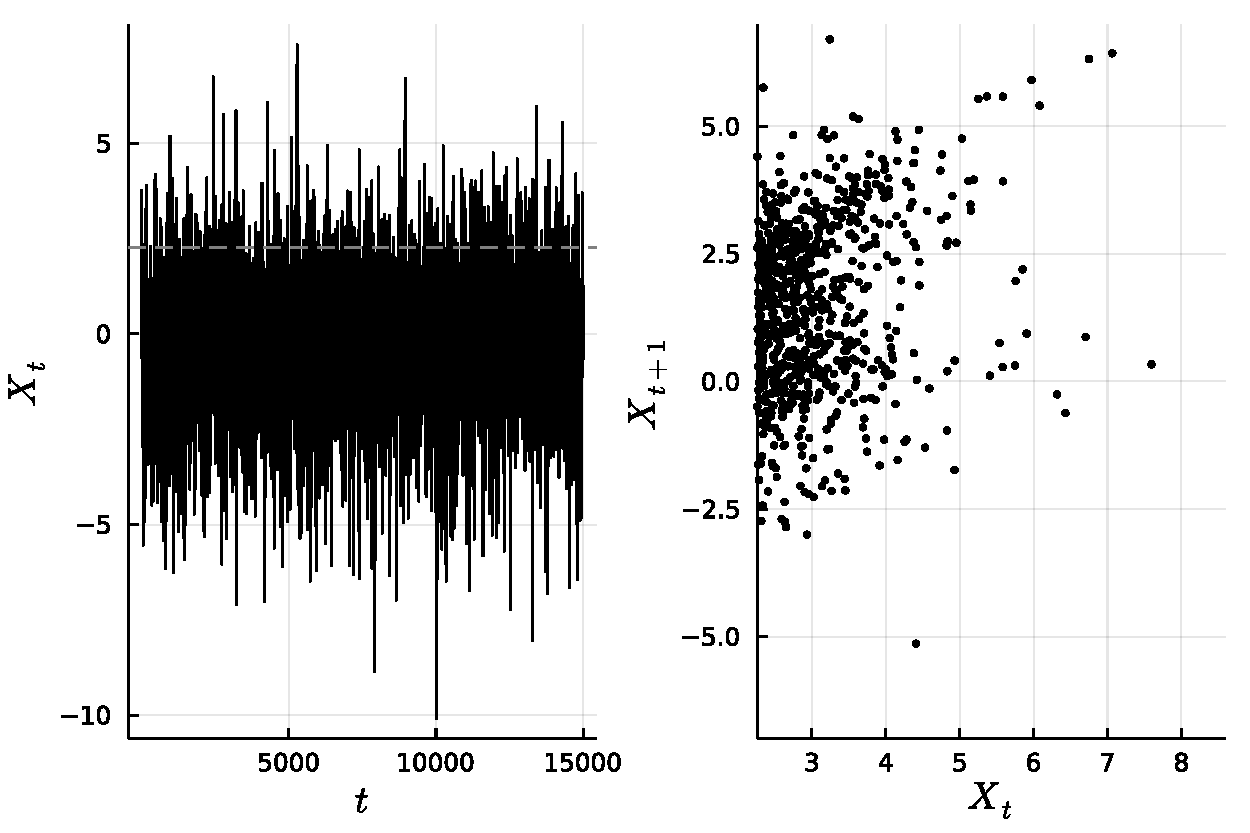
\includegraphics[scale=0.75]{../ht-em/figures/block_bootstrap_Xs.pdf}
  \caption{The left plot shows a time series of length 15000 generated from
  the 3 dimensional asymmetric logistic process, placed in Laplace margins. The
grey dashed line is $u$. The right plot shows $\D$.}\label{fig:block_bootstrap_Xs}
\end{figure}

Regarding the bootstrap, we reach in particular for the moving block
bootstrap~\citep{kunsch1989jackknife}, which can be applied to bootstrap stationary time series.
To explain how this can be applied to a CEVMM model,
suppose we have a time series $\{X_t\}_{t=1}^n$ and
that an appropriate threshold $u$ has been established. We form bootstrapped
series by sampling with replacement, $n/B$ times, blocks of size $B$ and then
concatenating these sampled blocks together to form bootstrapped series.
Repeating this $M$ times yields $M$ bootstrapped series
$\{\tilde{X}^j_{1:n}\}_{j=1}^M$.
A CEVMM can then be fit on each of the bootstrapped datasets
$\tilde{\D}^j := \{(\tilde{X}^j_{t},\tilde{X}^j_{t+1})\,|\,t=1,\ldots,n-1,\tilde{X}^j_{t}>u\}$,
which allows us to construct empirical confidence intervals on estimators
of interest.
The `moving block' aspect
comes from the fact that the set to be sampled from is $\{X_{1:B},X_{2:B+1},\ldots,X_{n-B+1:n}\}$.
A crucial assumption of the moving block bootstrap is that the original series $\{X_t\}$ from
which blocks are formed is stationary; since otherwise the resulting bootstrapped
series will not be comparable to the original series and any statistical analysis
will therefore be meaningless.

\FloatBarrier
Figure~\ref{fig:block_bootstrap_params} shows empirical distributions of fitted
parameters, generated using the moving
block bootstrap. It is promising that these empirical distributions corroborate
with the theoretically expected values of $\alpha_1,\,\alpha_2,\,\beta_1$ and
$\beta_2$. We see, however, that the distribution for $\alpha_2$ is slightly biased,
and that the bootstrap distribution for $\alpha_1$ places a small amount of mass near $0.8$.

\begin{figure}[htp]
  \centering
  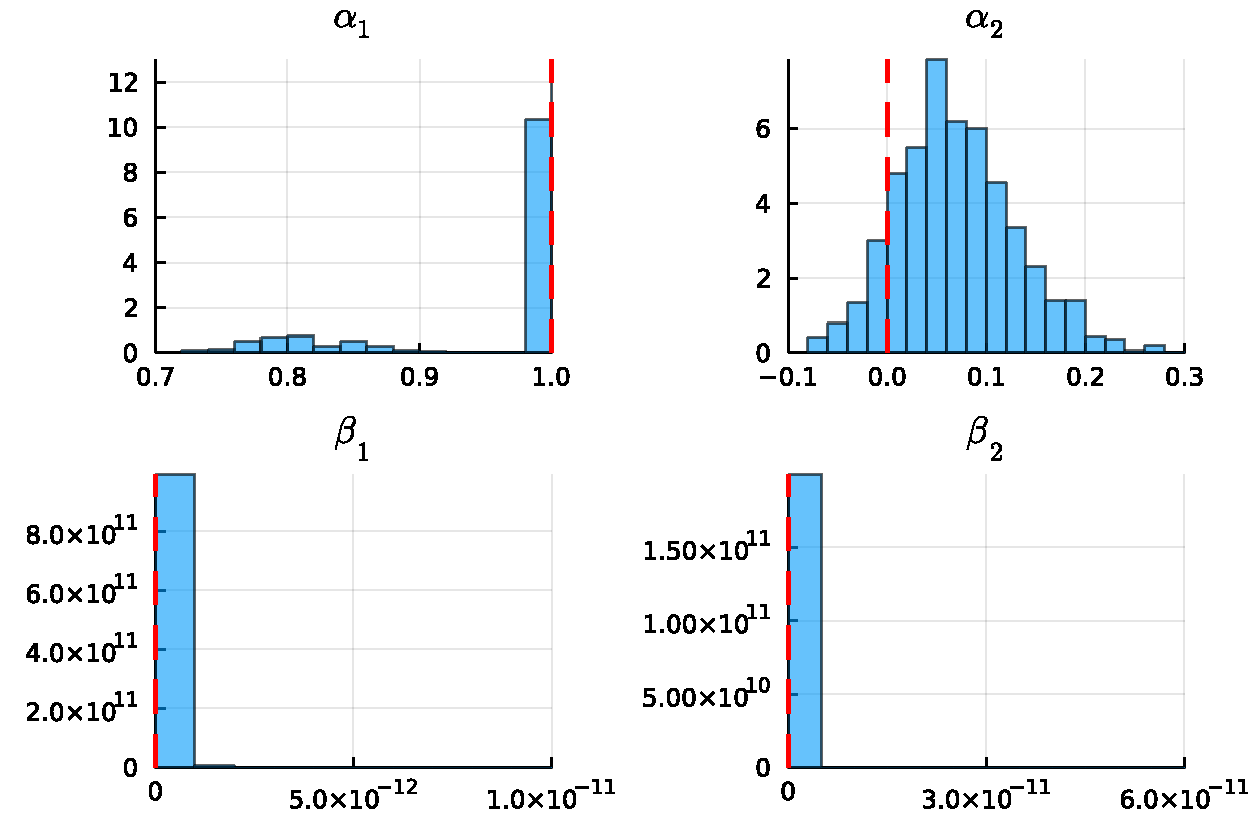
\includegraphics[scale=0.75]{../ht-em/figures/block_bootstrap_params_final.pdf}
  \caption{Histograms of fitted values $\alpha_1$, $\alpha_2$, $\beta_1$ and $\beta_2$ on $M=1000$ moving-block-bootstrapped time series with block size $B=50$. The parameter values fitted
on the full dataset are shown in red.}\label{fig:block_bootstrap_params}
\end{figure}

\FloatBarrier
Now that we have bootstrapped $M=1000$ models, we
can establish, as an example,
confidence intervals for $\hat F_{1|0}(\cdot;x_0)$. These have been calculated
and appear to work reasonably well for $x_0\leq F_0^{-1}(0.99)$
(Figure~\ref{fig:block_bootstrap_Fs_final}), even if
the confidence regions are perhaps a bit narrow for 99\% confidence.
Notice that there is no guarantee that estimators derived from the model fit on the full data will actually lie
in the bootstrapped confidence interval. This may be problematic. If this happens,
it suggests that the chosen $u$ is not suitable, or the model assumptions do not hold.
As we take $x_0$ larger in $\hat F_{1|0}(\cdot;x_0)$, we begin to
see a bias (Figure~\ref{fig:block_bootstrap_Fs_final_bad_large}).
The bias is more obvious when $x_0$ is large because the modes of the
distribution are further apart. Any error in the probability
assigned to each mode leads to a discrepancy where the CDF flatlines.

From what we have seen, these bootstrap confidence intervals for $\hat F_{1|0}$
should be taken lightly. This is not a huge surprise, since we have not shown
any underlying theory to support their use. However, they may still be of
practical use, in particular when conditioning on smaller values of $x_0$.
Having said this, the bootstrap distributions for the model parameters seem
more convincing. It would be interesting to implement a Bayesian CEVMM model
and compare associated confidence regions to these bootstrap confidence intervals,
but this is an area for future work.

\begin{figure}[htp]
  \centering
  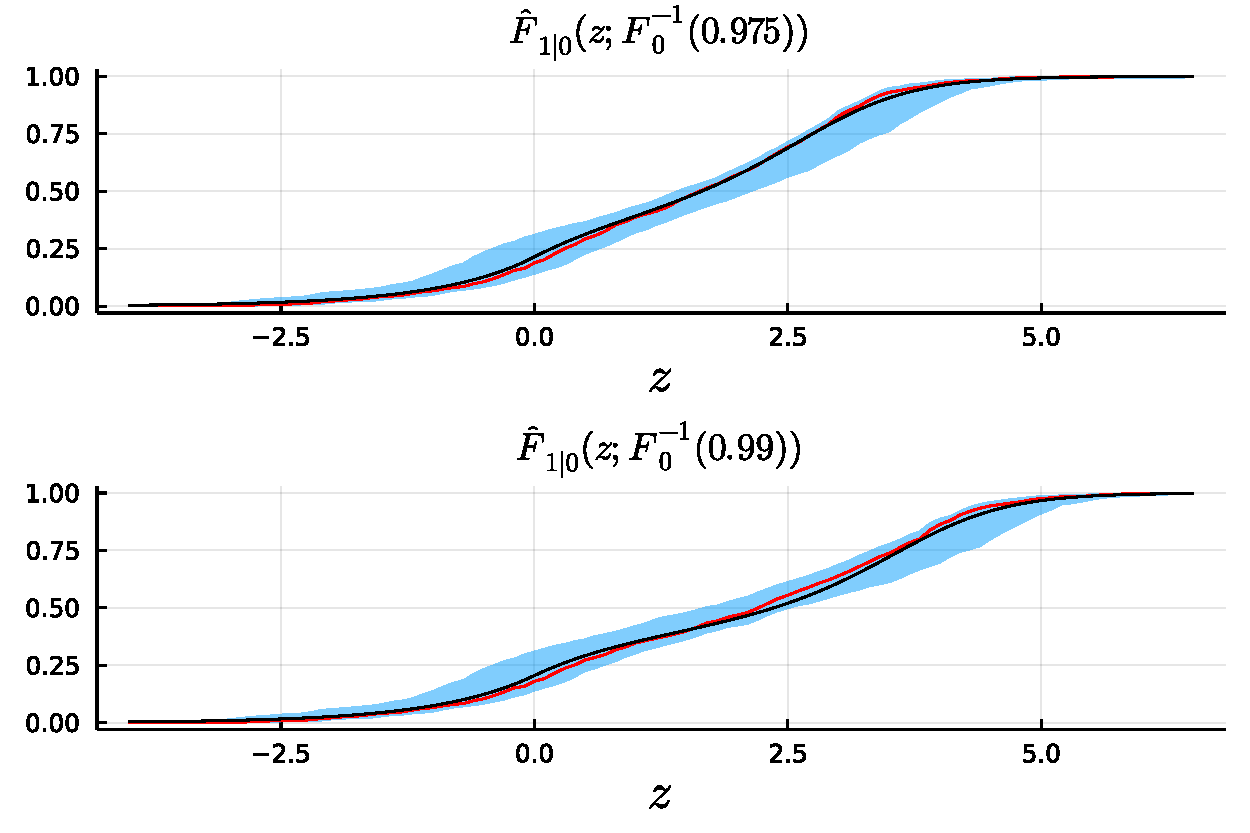
\includegraphics[scale=0.75]{../ht-em/figures/block_bootstrap_Fs_final2.pdf}
  \caption{Estimates for $F_{1|0}(x;x_0)$, for two large $x_0$.
    The true distribution is shown in black, and the distribution estimated from the full data shown in red.
    The 99\% confidence intervals, generated using $M=1000$ bootstrap samples, are shown in blue.}
    \label{fig:block_bootstrap_Fs_final}
\end{figure}

\begin{figure}[htp]
  \centering
  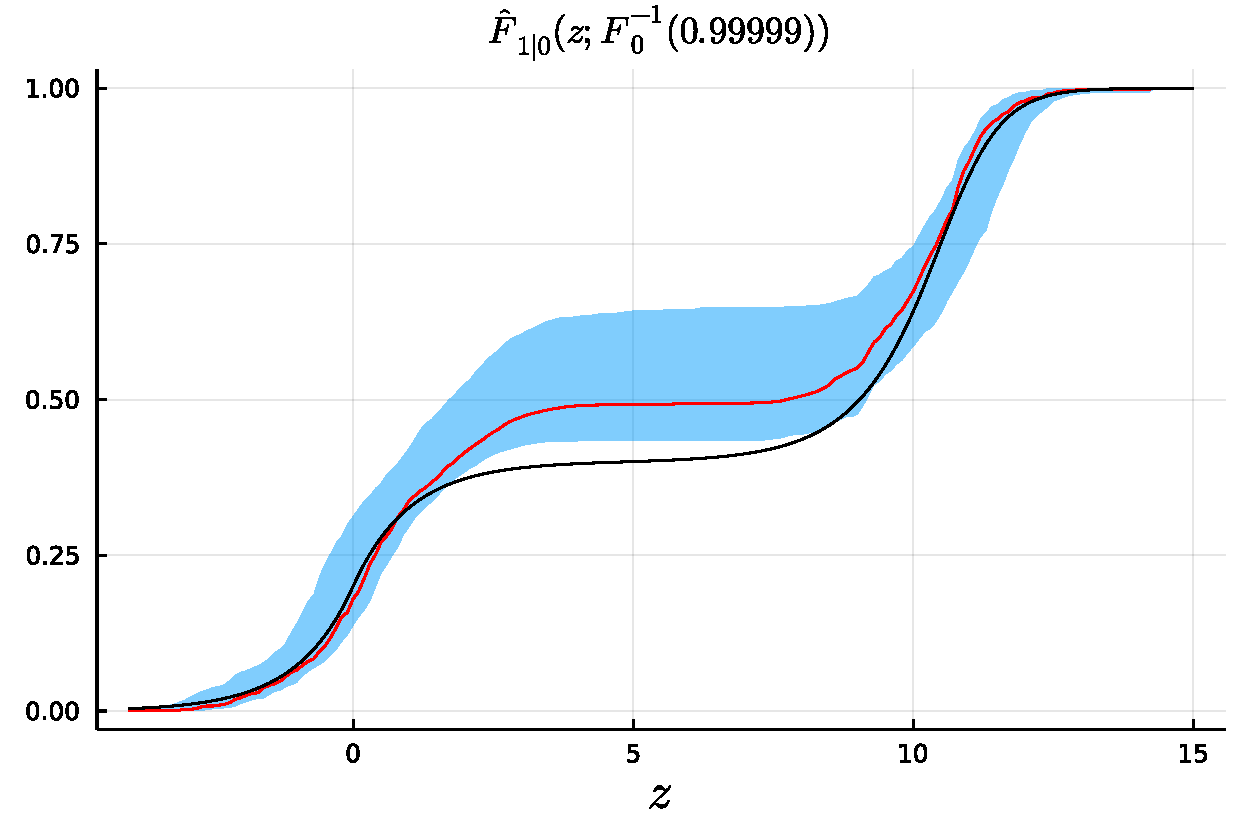
\includegraphics[scale=0.75]{../ht-em/figures/block_bootstrap_Fs_final_bad_large2.pdf}
  \caption{Estimate for $F_{1|0}(x;F_{0}^{-1}(0.9999))$.
    The true distribution is shown in black, and the distribution estimated from the full data shown in red.
    The 99\% confidence intervals, generated using $M=1000$ bootstrap samples, are shown in blue.}
    \label{fig:block_bootstrap_Fs_final_bad_large}
\end{figure}

\FloatBarrier

\section{Application to Electricity Imbalance Prices}

We apply the CEVMM methodology discussed above to electricity imbalance prices.
Because they can be very volatile, imbalance prices are a natural place to
apply extreme value statistics. We first give a short background on the UK
electricity markets, as this is necessary to understand the structure of
imbalance price data. We then perform a deseasonalization step to obtain
stationary-like residuals for model fitting. Finally, we fit a CEVMM on the
residuals and analyse the results.


\subsection{Background, and obtaining electricity imbalance price data}


It is in the interest of electricity suppliers and generators to strike
contracts with each other in order for them to supply electricity to their
customers, and to profit from electricity generation. In the UK,
there exist markets to trade these electricity contracts~\citep{liu2022evolution}
and in fact organisations that are neither suppliers nor generators can
participate~\citep{https://www.elexon.co.uk/about/bsc-explained/}.

Contracts will usually stipulate that the parties involved either consume or
produce a certain volume of electricity. In reality, parties will likely fail to
meet the contract requirements --- for example, a supplier may incorrectly predict the demand of its customers,
or the gales blowing on the eastern coast of Scotland may suddenly turn into
light breezes. The volume of electricity that does not balance in these
contracts, the imbalance, must be bought or sold on the central
electricity grid at a certain price. This price, typically
measured in £ per MWh, is determined half-hourly by
Elexon (\url{https://elexon.co.uk}), and is called the {\it imbalance price}.
Intuitively, we can expect the imbalance price to be high when there is
a high demand for electricity, but there is little supply on the central grid,
incentivising electricity generators to produce more. Conversely, we expect
a low imbalance price when there is excess power on the central grid -- it is even
possible for imbalance prices to be negative.

Imbalance price data is not available to download directly. However, it is
possible to obtain it via Elexon's API. There is a Python library
(\url{https://github.com/MichaelKavanagh/elexon}) to assist with this.
Imbalance volume data is also collected for each period --- this is
the total imbalance over all contracts in a particular period.

\subsection{Cleaning imbalance price data}\label{sec:cleaning_imbalance}

A graphical representation of the raw 2021 data can be found in
Figure~\ref{fig:whole_year_imbalance_price}. The year 2021 had 365 days, and we have 48
periods per 24 hours, so we expect to work with an imbalance price time series of
length 17520.

Unfortunately, price data is missing from 2021-06-23 for periods 34 and 37
(there were no other missing data). Mean imputation was used to impute these
missing values (the mean prices were calculated using data from the same month, June, and from the same
periods). While multiple imputation is generally preferable to mean imputation, it is not
expected that these values will actually affect the final CEVMM model since
from Figure~\ref{fig:whole_year_imbalance_price} we see that it is unlikely June will have
extreme values in the upper tail.

We later model the imbalance prices in order to extract residuals (see~\eqref{eq:select_imb_model} for the final model used). In particular we
use $\code{period}\in\{1,\ldots,48\}$ as a covariate, which is complicated by
the UK switching time zones to/from UTC from/to BST for daylight savings. The
upshot of this is that 2021-03-28 has 2 fewer periods and 2021-10-31 has 2 more
periods than other days. To work around this, the missing values in March are
mean imputed, and the data corresponding to periods 49 and 50 in October are
dropped. Imbalance volumes are imputed in a similar way in March.


To avoid massive outliers in the imbalance price, we perform a log transformation on the
price, namely $\code{log_price'}:= \log(\code{price} + a)$, where \code{price} denotes the imbalance price.
The adjustment term $a$ in the argument to the logarithm is to ensure that the argument is positive.
Though we are fitting models with 2021 data, for the purposes of compatibility with
2022 data (e.g.\ for prediction), we select $a=91=-\min\lceil\code{price}\rceil$,
where the $\min$ is taken over all periods between 2021-01-01 and 2022-08-01.
 Finally, we standardize the volumes and prices
to have mean 0 and standard deviation 1.

\FloatBarrier
\begin{figure}[htp]
  \centering
  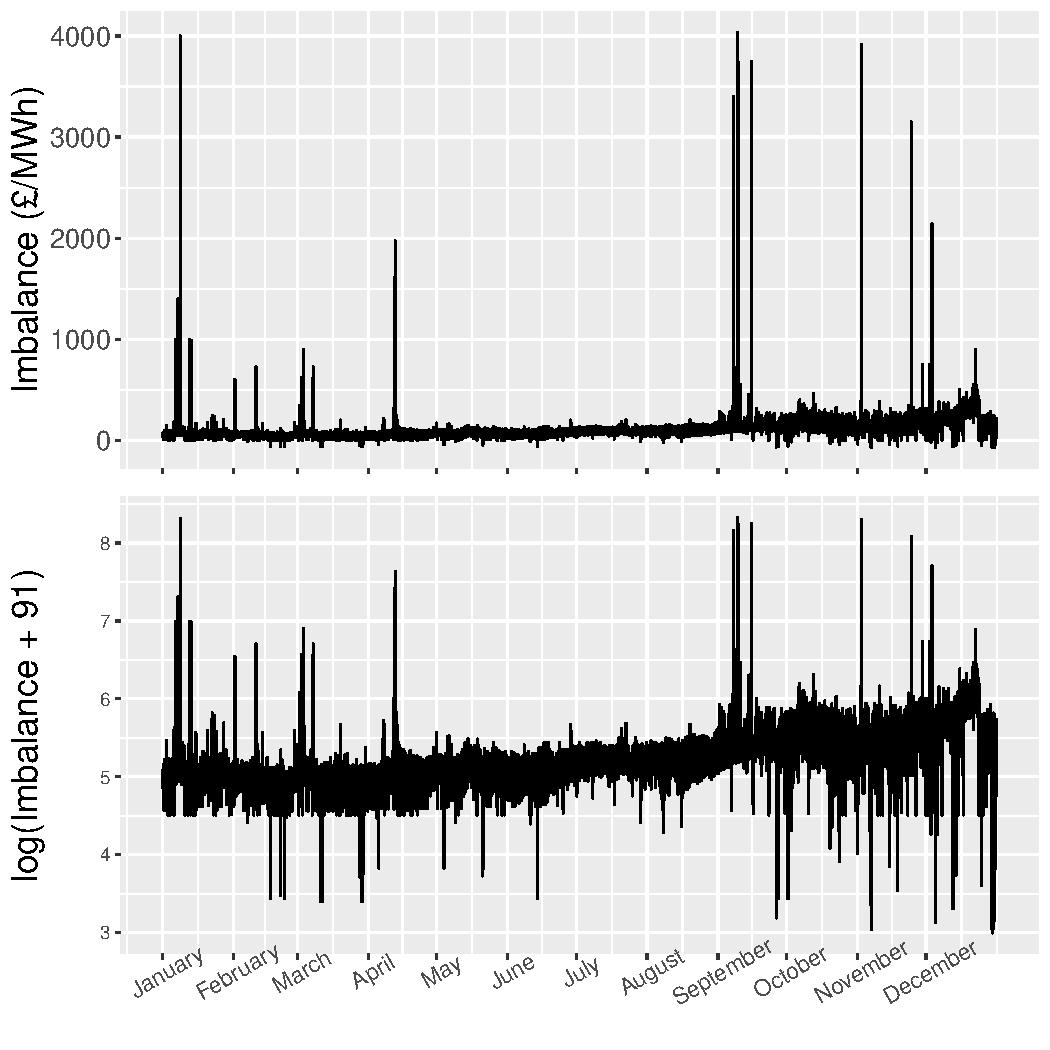
\includegraphics[scale=0.75]{../elexon/figures/imbalance_whole_year.pdf}
  \caption{Imbalance prices, and imbalance prices on a log scale, for
  2021. Months labelled correspond to the first period of the month.}\label{fig:whole_year_imbalance_price}
\end{figure}



\subsection{Seasonalizing imbalance prices}

Imbalance prices are seasonal. This is because
demand for electricity fluctuates throughout the day and throughout the
year. In order for i.i.d.\ assumptions to be valid when fitting CEVMM models,
we first fit a model on the imbalance prices in the hope of recovering
stationary residuals; we call this step {\it deseasonalization}.
We will then fit a CEVMM model on these residuals.
We begin with a simple linear model with the factors \code{weekday}, \code{month}
and \code{period}, given by
\begin{equation}\label{eq:seasonal_imbalance_price_factor}
  \begin{split}
    \code{log_price} &= \beta_0 + \beta_1 \cdot \code{weekday} + \beta_2 \cdot \code{month} + \beta_3 \cdot \code{period} + \eps\\
    \eps &\sim N(0,\sigma^2)\\
    \code{weekday}&\in \{\code{Monday},\ldots,\code{Sunday}\}\\
    \code{period}& \in \{1,\ldots,48\}\\
    \code{month}& \in \{\code{January},\ldots,\code{December}\}\\
    \text{where}&\\
    \code{log_price} &= \frac{\code{log_price'} - \text{mean}(\code{log_price'})}
    {\text{std}(\code{log_price'})}\\
    \code{log_price'} &= \log(\code{price} +a).\\
  \end{split}
\end{equation}
The log and standardization transforms are as discussed
in Section~\ref{sec:cleaning_imbalance}.
 A deseasonalization can then be obtained with $y :=
\code{log_price} - \widehat{\code{log_price}}$, of which a plot can be
found in Figure~\ref{fig:lprice_res_simple}. It is clear that large values of
$y$ correspond with high imbalance prices, and similarly small values
of $y$ correspond with low imbalance prices.
\clearpage



One issue, at least visually, with the residuals in
Figure~\ref{fig:lprice_res_simple} is the uptick towards the end of the
series, and then the sudden jump down. Some experimentation finds
that autoregressive terms help capture more variance. In particular,
we consider the following covariates

\begin{enumerate}[(a)]
  \item \code{last_log_price1} and \code{last_log_price2},
    the \code{log_price} of the previous and second to last period respectively;
  \item \code{last_quantity1} and \code{last_quantity2},
    the imbalance quantities of the previous and second to last
    period respectively;
  \item \code{yday_log_price} and \code{yday_quantity}, the \code{log_price}
    and imbalance quantity of the same period yesterday.
\end{enumerate}

Stepwise selection was used (with the AIC criterion) to find which terms to include,
with the selected model shown in~\eqref{eq:select_imb_model}.
Note that by introducing \code{yday_quantity} and \code{yday_log_price},
we have no residuals for 2021-01-01, meaning that there are 17472 residuals in total.
\begin{equation}\label{eq:select_imb_model}
  \code{log_price} = \begin{bmatrix}
    \code{yday_log_price} \\
    \code{last_log_price1}\\
    \code{last_quantity1}\\
    \code{last_log_price2}\\
    \code{last_quantity2}\\
    \code{period} \\
    \code{month} \\
    \code{weekday}\\
  \code{last_log_price2}\cdot\code{last_quantity2}
\end{bmatrix}^T\beta + \eps,\,\eps~\sim N(0,\sigma^2)
\end{equation}
Visually, the residuals for model~\eqref{eq:select_imb_model} look more
convincingly stationary
than the model defined by~\eqref{eq:seasonal_imbalance_price_factor}
(Figure~\ref{fig:lprice_res_stepwise} vs.\ Figure \ref{fig:lprice_res_simple}).
Note that in neither model is the normal assumption reasonable given the huge spikes seen
in the figures, but this is the behaviour we aim to capture later with the CEVMM model.

\FloatBarrier

\begin{figure}[htp]
  \centering
  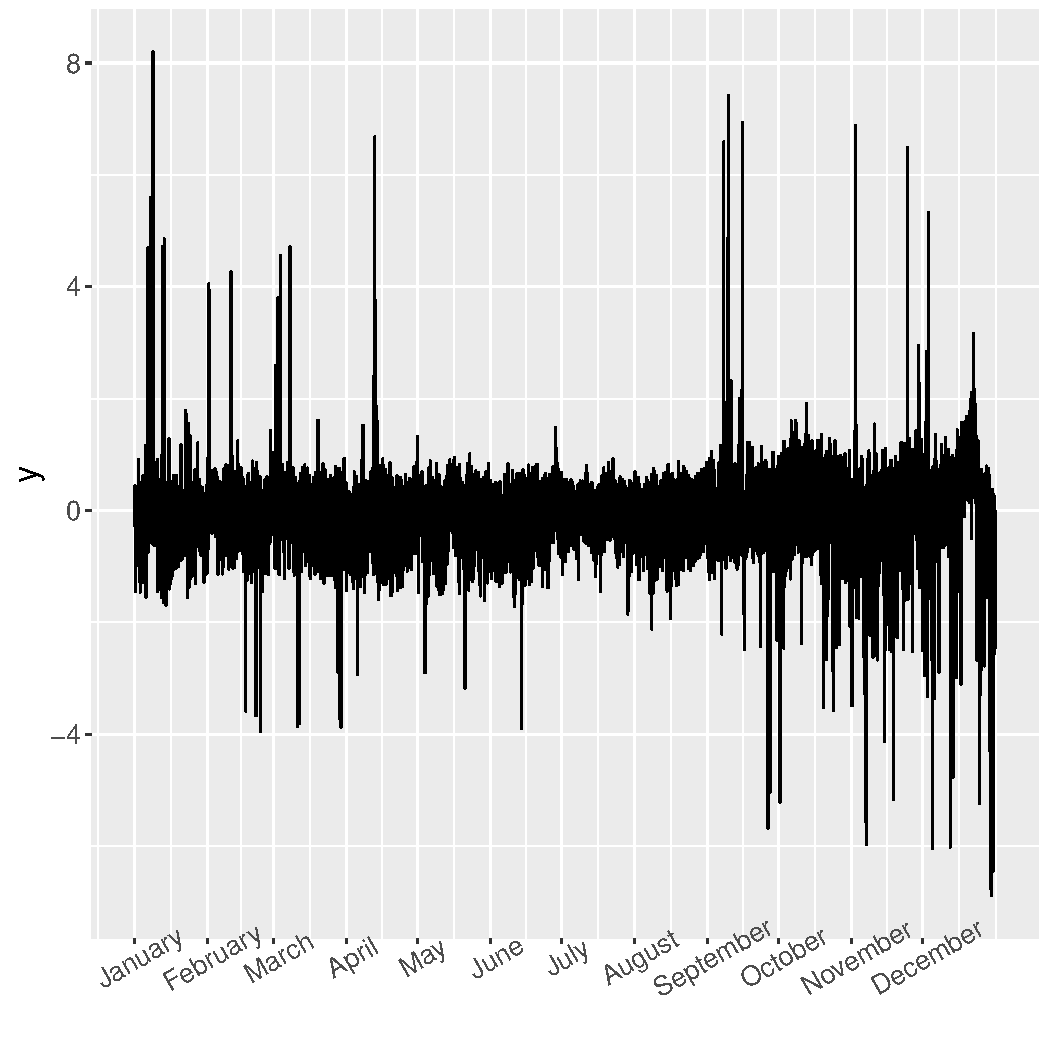
\includegraphics[scale=0.6]{../elexon/figures/y_resid.pdf}
  \caption{Plot of $y :=\code{log_price} - \widehat{\code{log_price}}$ vs.\ period
  for model~\eqref{eq:seasonal_imbalance_price_factor}. Months labelled
correspond to the first period of the month.}\label{fig:lprice_res_simple}
\end{figure}

\begin{figure}[htp]
  \centering
  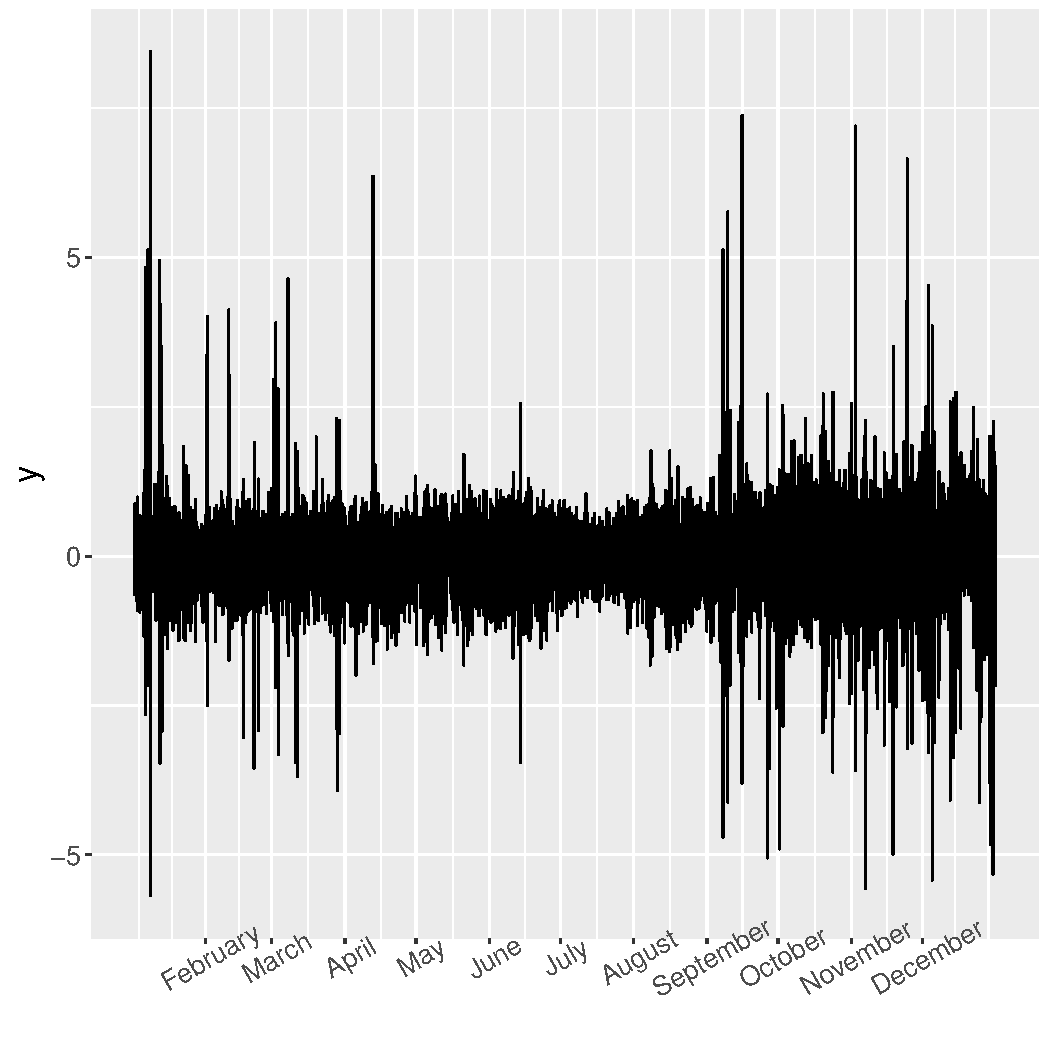
\includegraphics[scale=0.60]{../elexon/figures/y_lm_final.pdf}
  \caption{Plot of $y :=\code{log_price} - \widehat{\code{log_price}}$ vs.\ period for model~\eqref{eq:select_imb_model}, chosen using stepwise selection. Months labelled
correspond to the first period of the month.}\label{fig:lprice_res_stepwise}
\end{figure}
\FloatBarrier

To quantitatively check that $y$
actually resembles {\it something} like a deseasonalization, we run a KPSS test
 to check for level stationarity.

\verbatiminput{../elexon/kpss-result/lm-final.txt}

Model~\eqref{eq:select_imb_model} is not perfect as
there is not overwhelming evidence for stationarity of its residuals.
However, there is also no evidence against stationarity by the KPSS test above.
Since we are mostly interested in applying a CEVMM model, we consider
this model sufficient.

As a final note on deseasonalization, we point out that there is one clear
disadvantage of moving from the simpler
model~\eqref{eq:seasonal_imbalance_price_factor}
to~\eqref{eq:select_imb_model}. The residuals of the latter model no longer
have a simple interpretation in terms of the price imbalance
because the residuals are now coupled to the imbalance volume, as well as
the imbalance price. This, unfortunately, reduces interpretability.

\subsection{Fitting the CEVMM model}

Given deseasonalized residuals of the imbalance data $\{y_t\}_{t=1}^{17472} =
\{\code{log_price} - \widehat{\code{log_price}}\}$,
we first move them to Laplace margins so that we can fit a CEVMM model.
We choose Laplace margins over logistic margins as a result of the experiments
of Section~\ref{sec:lap_vs_log}.
Since the distribution of the residuals is unknown, we apply
the transformation $y_t \mapsto F^{-1}_{\text{Laplace}}[n/(n+1)\hat F_{\text{ecdf}}(y_t)]$
to map to approximate Laplace margins. The factor $n/(n+1)$ is necessary to
avoid the largest residual being mapped to the upper end point $F_{\text{Laplace}}^{-1}(1) = \infty$.


Figure~\ref{fig:imb_first_order_tail} shows the raw data, where it is
possible to see at least 2 modes for $y_{t} | y_{t-1} > u$.
One mode corresponds to positive dependence, $\mathrm{corr}(y_{t-1},y_{t}) > 0$,
and the other mode corresponds to negative dependence. This leads us to assume that
there are $K=2$ modes.

\begin{figure}[htp]
  \centering
  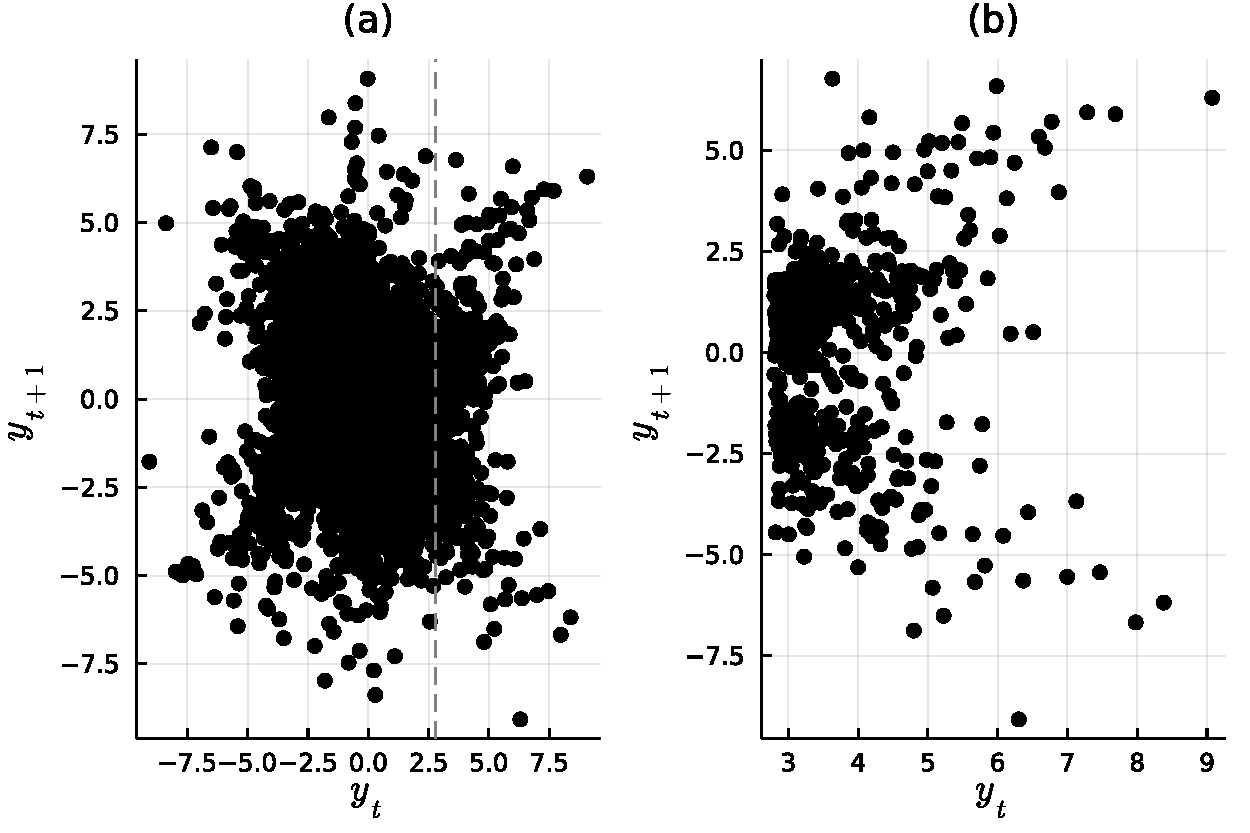
\includegraphics[scale=0.75]{../elexon/figures/first-order-raw.pdf}
  \caption{Plots of $y_t$ vs.\ $y_{t-1}$ (Laplace margins). $(a)$ shows all the data,
    with the dotted line denoting $y_{t-1}=u=2.8$; (b) focuses on the region $y_{t-1}>u$.}\label{fig:imb_first_order_tail}
\end{figure}

We first set the regularization parameter to $\gamma=0.05>0$ as
$\gamma = 0$ leads to overfitting ($\gamma = 0.05$ in particular was chosen
because it was found to have worked well for asymmetric logistic data).
See Figure~\ref{fig:seed_18} and the corresponding
parameter estimates in Table~\ref{table:seed_18} as an example of this overfitting.
We see that the data has not been
clustered naturally, and the table shows that the fitted variances
are perhaps artificially small.

\begin{table}[htp]\centering
  \begin{tabular}{c |c |c |c |c |c |c |c |c |c}
$\hat\pi$ & $\hat\alpha_1$ & $\hat\alpha_2$ & $\hat\beta_1$ & $\hat\beta_2$ & $\hat\mu_1$ & $\hat\mu_2$ & $\hat\sigma_1$ & $\hat\sigma_2$ & Log likelihood \\
    \hline
  0.4374 & 1.0000 & -0.9994 & 0.6515 & 1.0000 & -0.9555 & 0.7594 & 0.2632 & 0.6768 & -1674.3615 \\
\end{tabular}
 \caption{Best CEVMM fit of 30 random initial values, with no regularization and $u=F_{\text{Laplace}}^{-1}(0.95)$.\label{table:seed_18} }
\end{table}

\begin{figure}[htp]
  \centering
  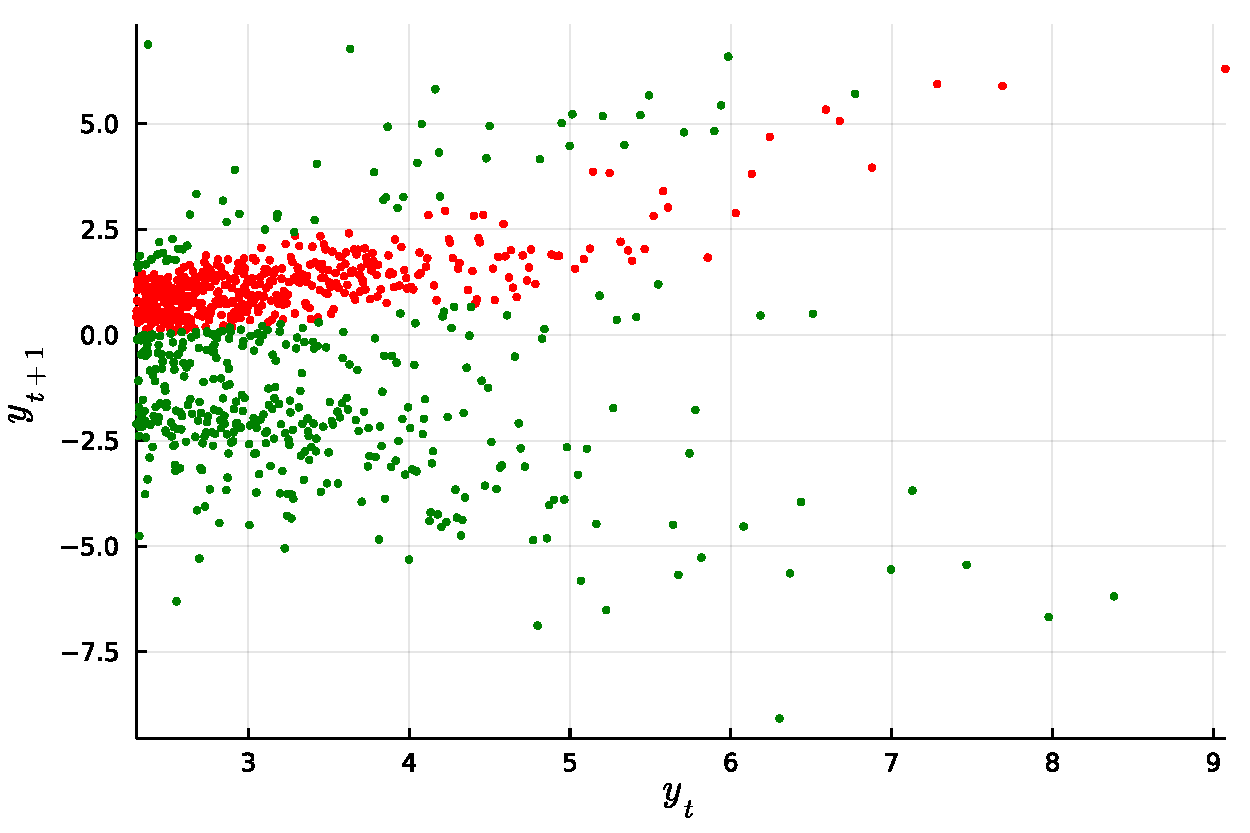
\includegraphics[scale=0.75]{../elexon/figures/seed_18.pdf}
  \caption{Best CEVMM fit of 30 different models each fit with random initial values.
    Here, $\gamma=0$ and $u=F_{\text{Laplace}}^{-1}(0.95)$. Data points are colour coded according to which normal mixture they most
likely belong to.}\label{fig:seed_18}
\end{figure}

\FloatBarrier
It is not obvious which value should be chosen for the threshold $u$.
We proceed by fitting CEVMMs for several $u\in[1.6,3.9]\approx
F_{\text{Laplace}}^{-1}([1.6,3.9])$. Figure~\ref{fig:imb_param_vals_changing_u}
shows how the fitted values change with $u$ --- we select $u=2.8$
since for $u<2.8$ we see $\alpha_1$ steadily decreasing and $\mu_2$ steadily increasing.

\begin{figure}[htp]
  \centering
  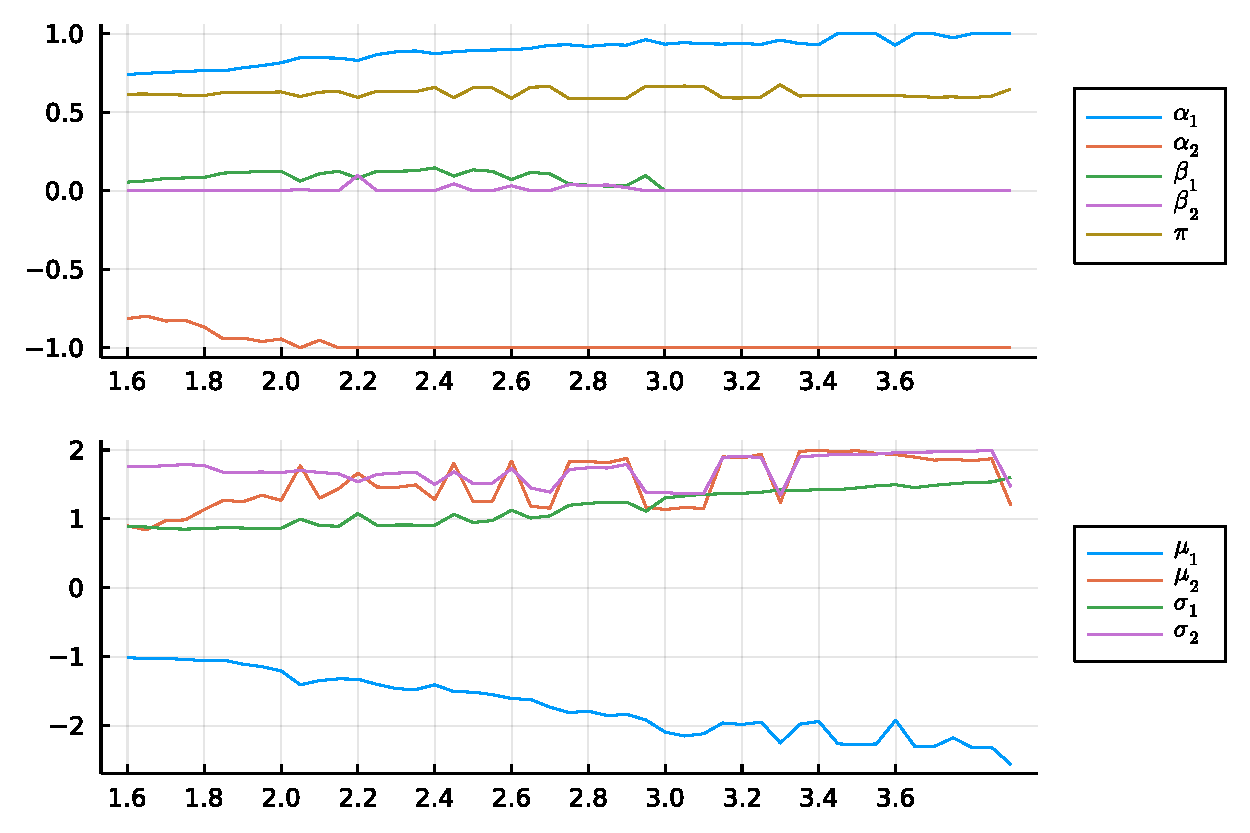
\includegraphics[scale=0.75]{../elexon/figures/imb_param_vals_changing_u.pdf}
  \caption{Effect of threshold $u$ on the fitted parameters, with $\gamma=0.05$.}\label{fig:imb_param_vals_changing_u}
\end{figure}

Figure~\ref{fig:imb_contour_with_reg05} and Table~\ref{table:imb_reg05} show
the fitted model with the selected parameters. We see a much more natural separation
of the modes, and most data points are being clustered to the mode that one might expect.

%There is a question of whether data points with $y_{t+1} \approx 0$ ought to be
%assigned to the upper mode or lower mode --- binary classification may be too
%reductionist here. It is proposed to sample several ECDFs when forming
%the model~\eqref{eq:ht_mix_final}, by sampling the classifications of each data
%point, as in Section~\ref{sec:cevvm_uncertainty}.

\begin{table}[htp] \centering
  \begin{tabular}{c |c |c |c |c |c |c |c |c |c}
$\hat\pi$ & $\hat\alpha_1$ & $\hat\alpha_2$ & $\hat\beta_1$ & $\hat\beta_2$ & $\hat\mu_1$ & $\hat\mu_2$ & $\hat\sigma_1$ & $\hat\sigma_2$ & Log likelihood \\
    \hline
  0.6702 & 1.0000 & -1.0000 & 0.0000 & 0.0000 & -2.3069 & 1.1855 & 1.2633 & 1.4060 & -1126.2791 \\
\end{tabular}
 \caption{Fitted parameter values and log
  likelihood for $K=2$, $\gamma=0.05$, $u=2.8$.\label{table:imb_reg05}}
\end{table}

\begin{figure}[htp]
  \centering
  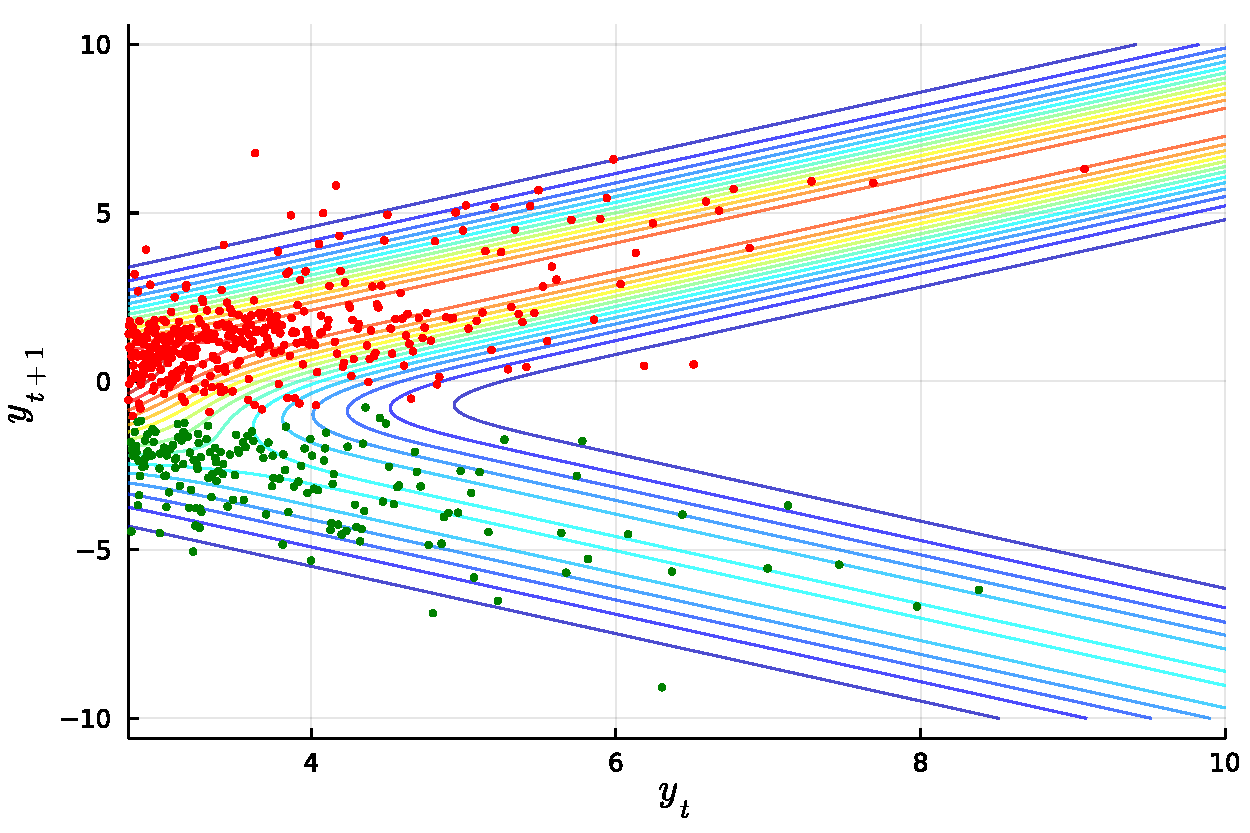
\includegraphics[scale=0.75]{../elexon/figures/imbalance_contour_with_reg05.pdf}
  \caption{CEVMM fit, with regularization $\gamma=0.05$ and $u=2.8$. Data points are colour coded according to the normal mixture they most likely belong to. The coloured
    lines show contours of the modelled normal mixture density
    for $y_{t+1}|y_{t}$, when viewed as a function of both $y_{t+1}$ and $y_{t}$.}\label{fig:imb_contour_with_reg05}
\end{figure}

\subsection{Uncertainty in model parameters}

Using the moving block bootstrap once again, as in Section~\ref{sec:cevvm_uncertainty}, we can
estimate uncertainty in the fitted parameters. Figure~\ref{fig:parameter_uncert_k2}
shows estimated distributions for $M=1000$ bootstrap replications.
A block size $B=48$ was used for convenience, as 48 divides the total length of the
time series $\{y_t\}$ evenly.
The samples clearly corroborate with the values fitted on the full dataset and
there is little uncertainty. However,
the small islands of mass away from the parameter boundaries are suspect.
We saw similar behaviour with the asymmetric logistic data in
Figure~\ref{fig:block_bootstrap_params}. It may be that there are
a few data points in the dataset that are influential in encouraging
the parameters to the boundary, and sometimes they are not included by the bootstrap.


\begin{figure}[htp]
  \centering
  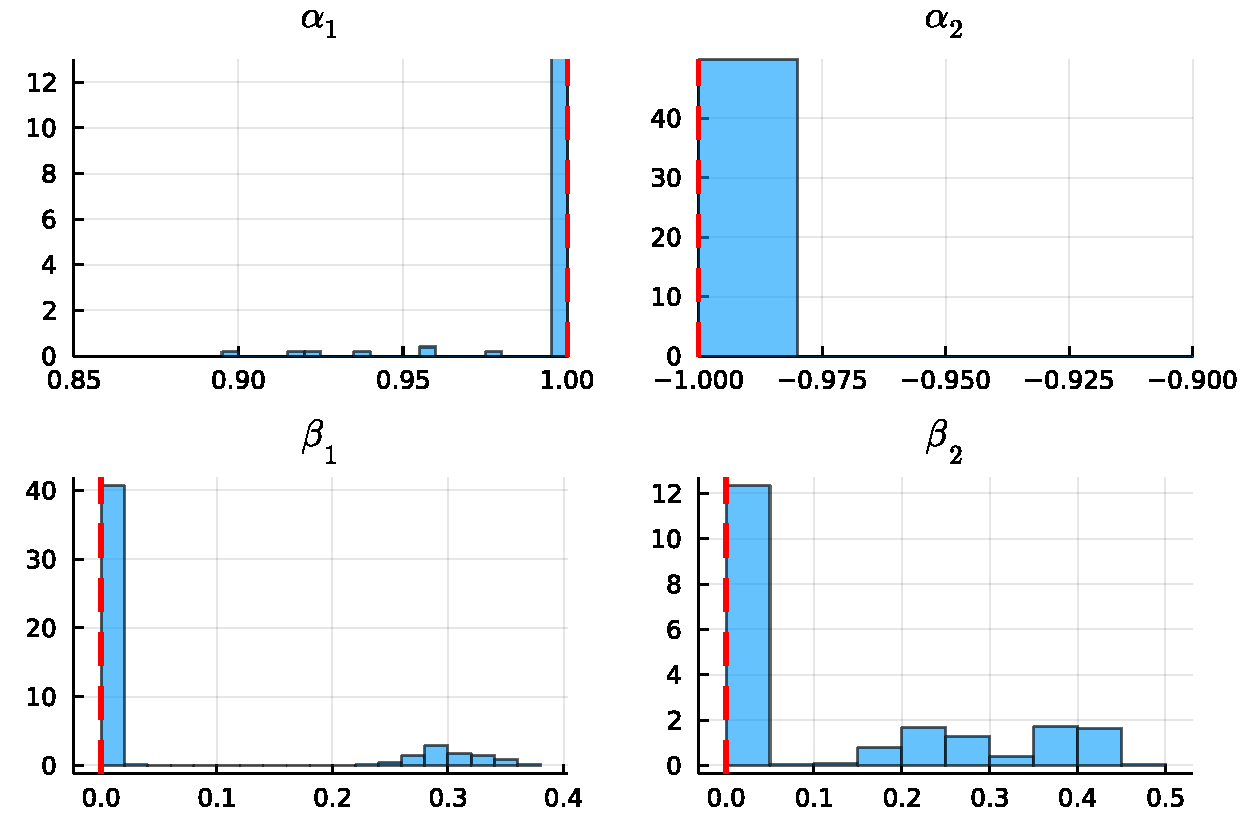
\includegraphics[scale=0.7]{../elexon/figures/parameter_uncert_k2.pdf}
  \caption{Histograms of fitted values $\alpha_1$, $\alpha_2$, $\beta_1$ and $\beta_2$ on $M=1000$ moving-block-bootstrapped time series with block size $B=48$. The parameter values fitted
on the full dataset are shown in red.}\label{fig:parameter_uncert_k2}
\end{figure}

\FloatBarrier
\subsection{One-step-ahead residual prediction}

If the current price's residual $y_t=y$ is large, then it is simple to use a CEVMM to find
a one-step-ahead predictive distribution for the imbalance price residuals.
We demonstrate this with the above CEVMM model (defined by parameters in Table~\ref{table:imb_reg05})
by finding predictive distributions for January 2022 data.

Concretely, one-step-ahead prediction means sampling from $\hat F_{1|0}$,
as we assume that $y_{t+1}|y_{t} \sim F_{1|0}(\cdot\,;\,y_t)$.
Note that the procedure does not take into account uncertainty in the CEVMM
model's parameters.
This
is a good test case because the data is out-of-sample for the CEVMM model,
and additionally the true residuals are known, so it is possible to assess the
performance of our predictions.

Imbalance price residuals for January 2022 (after the usual transformation to Laplace
margins) are shown in Figure~\ref{fig:jan22_resids} (of which there are
$48\cdot31 = 1488$), and the results of sampling predictions are
shown in Figure~\ref{fig:jan22_hists_22} for the first 16 exceedances (out of 45).
%The `true' residual is shown in red, and a point estimator for $y_{t+1}$ from an ARIMA model
%(fit the residuals) is shown in green for comparison.


We can see that when predicting one step ahead, the CEVMM assigns
a larger probability to the upper mode than the lower mode.
See Figure~\ref{fig:jan22_hists_22};
sometimes the upper mode is a good predictor (e.g.\ row 1, column 3);
sometimes the lower mode is a good predictor (e.g.\ row 2, column 2),
and sometimes neither are good estimators (e.g.\ row 3, column 4).
As such, the CEVMM model is not going to be useful for
constructing point estimates, but more for managing risk.
The ARIMA predictions are plotted merely out of interest, but it illustrates
that more standard time series model tend not to predict such large residuals
as the CEVMM model, even when they are likely to happen.
The estimate from the ARIMA model tends to be more conservative than the CEVMM model.

\begin{figure}[htp]
  \centering
  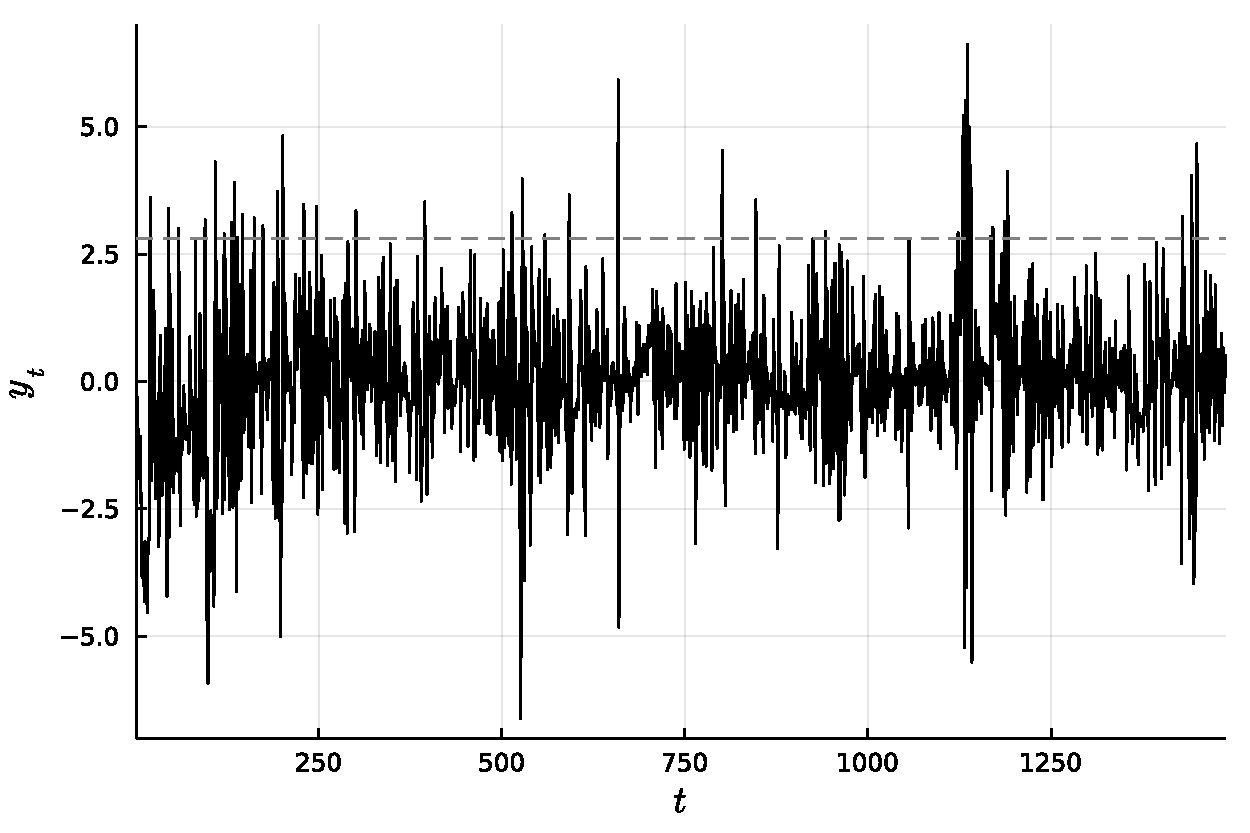
\includegraphics[scale=0.70]{../elexon/figures/resids_jan_22.pdf}
  \caption{Imbalance price residuals for January 2022, with threshold $u=2.8$ shown by the grey dashed line.}\label{fig:jan22_resids}
\end{figure}



We repeat the above for $K=3$; the model used has parameters detailed in
Table~\ref{table:k_3_fits}. The results are shown in
Figure~\ref{fig:jan22_hists_k3}. We compare the two values of $K$ by looking at
their predictive capabilities.
The proxy we use is likelihood of the data, where the likelihood
is determined by a Gaussian kernel density estimator; that is, we fit density
estimator on the simulated residuals of $y_{t+1}|y_{t}$, for each of
the 45 exceedances in January 2022, and calculate likelihoods of the actual
values. We compare the distributions of these likelihoods in Figure~\ref{fig:k2_k3_violin}. The distribution of likelihoods
looks similar, but $K=2$ has a
slightly higher mean, and also has a higher `best likelihood'.
Overall, there is no reason to prefer $K=3$.


\begin{figure}[htp]
  \centering
  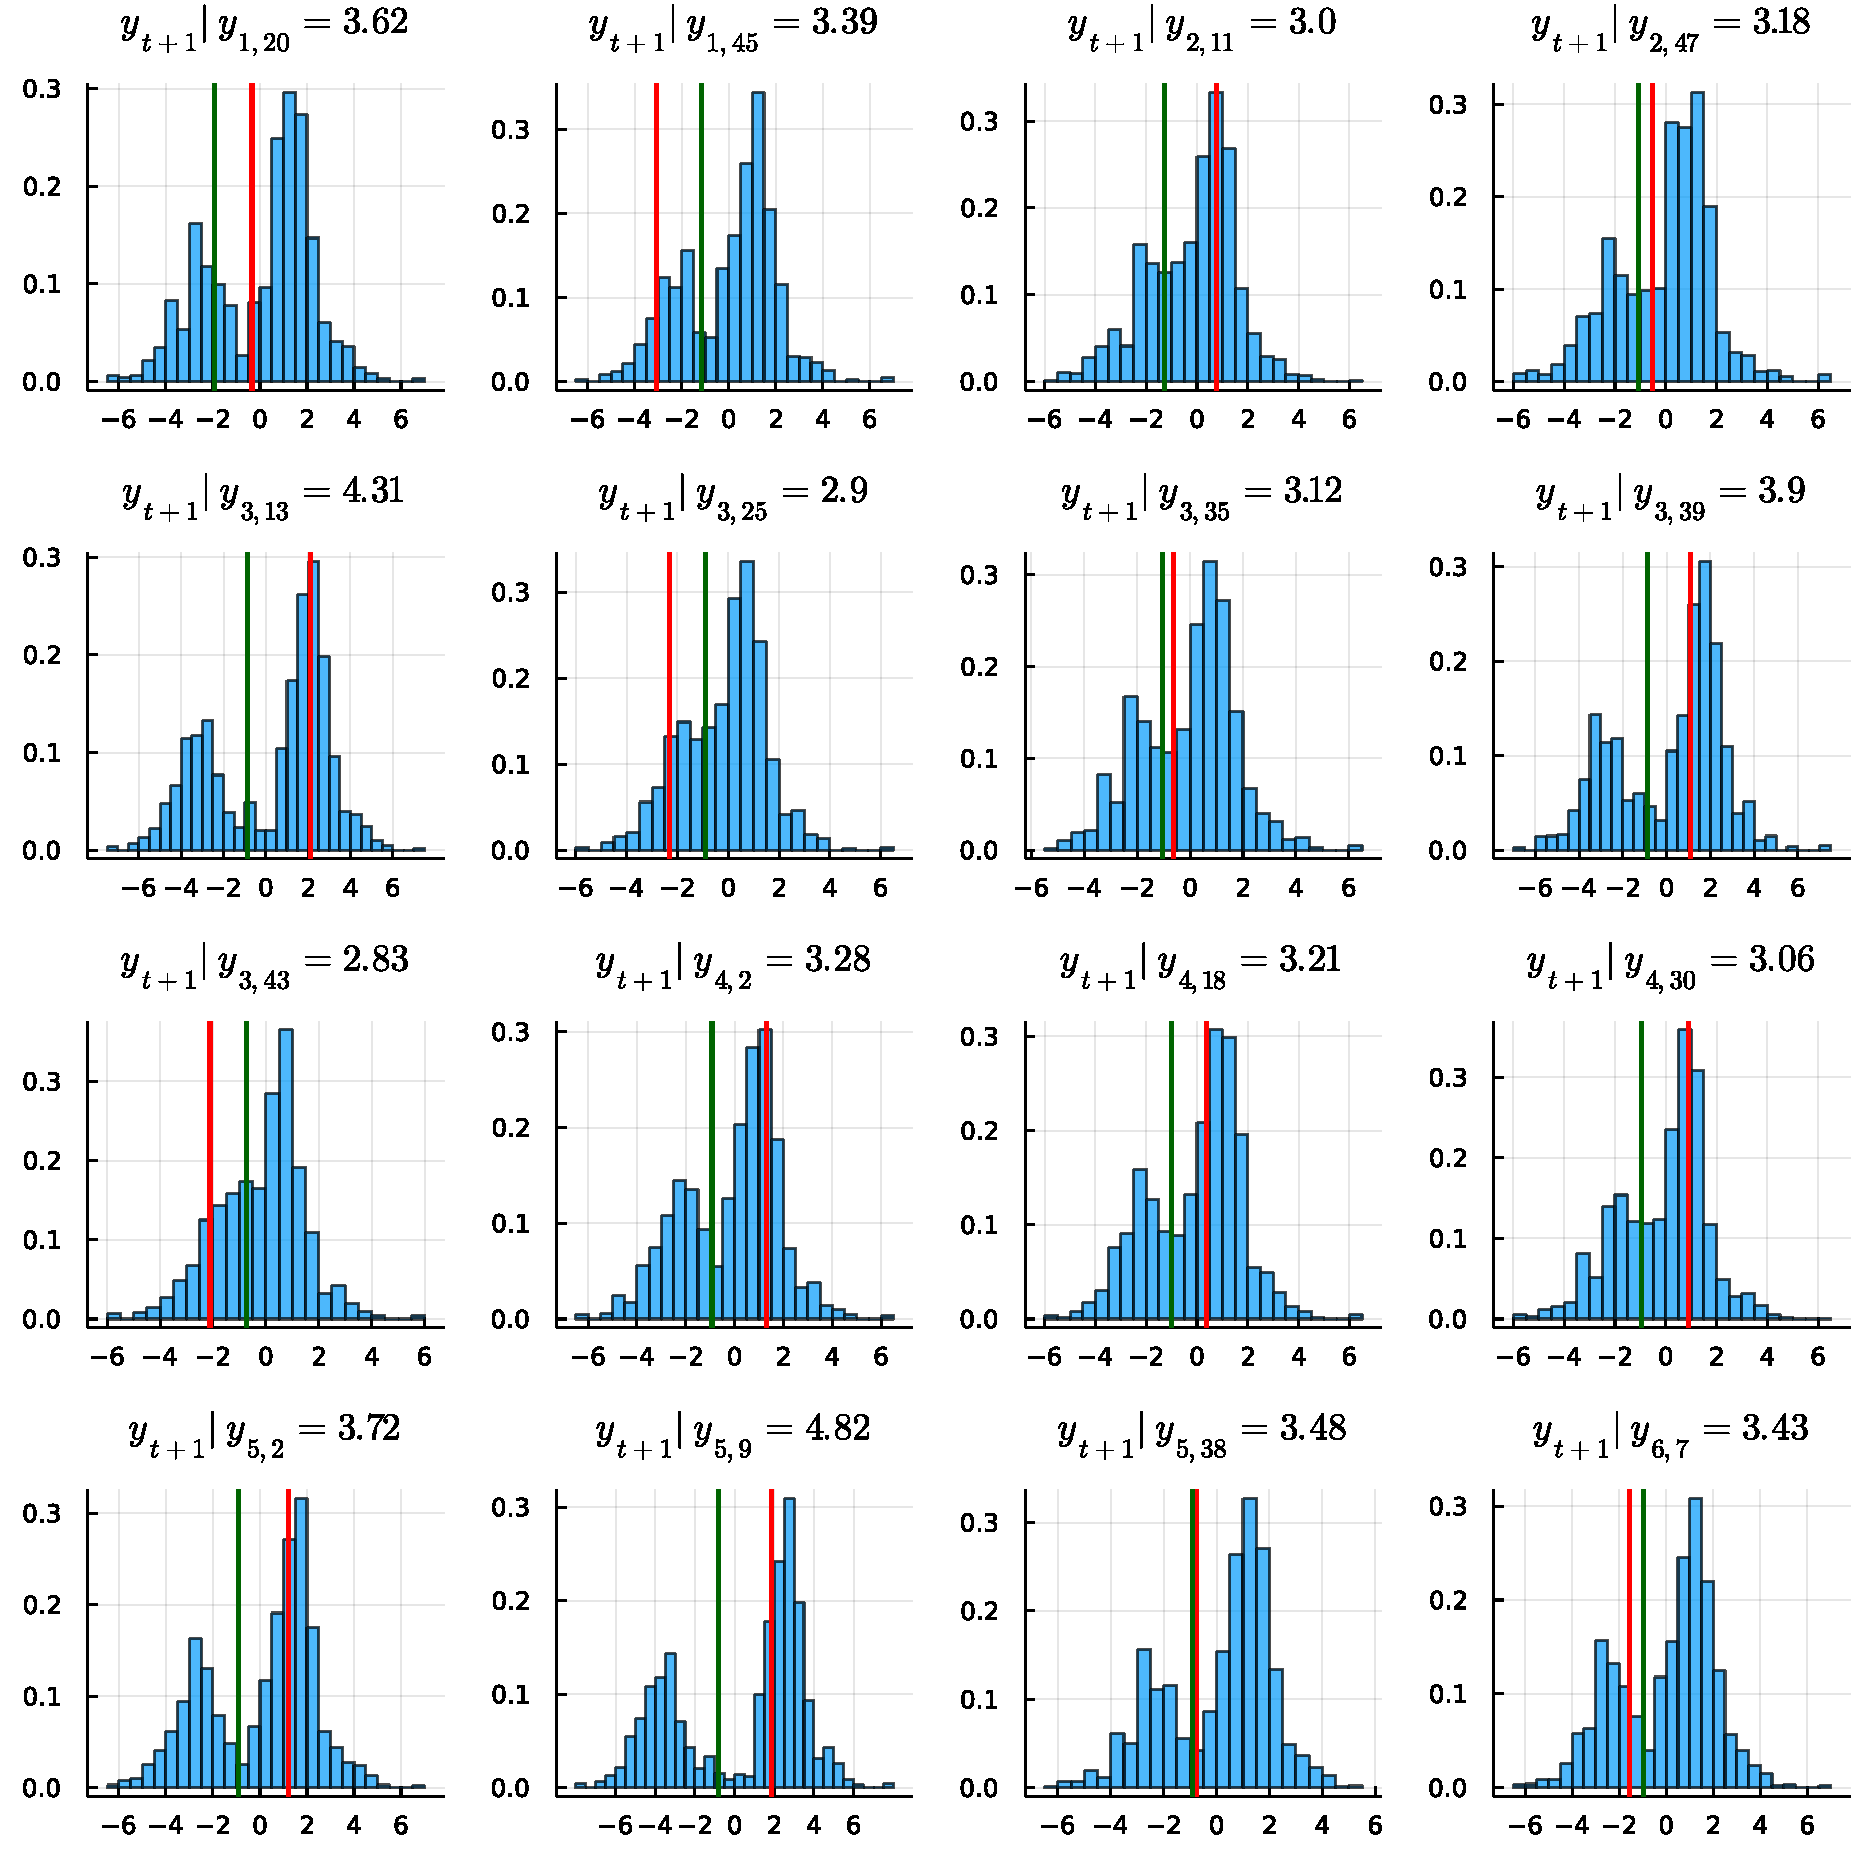
\includegraphics[scale=0.5]{../elexon/figures/ytp1_giv_yt_jan_22_k2_full_pred_final.pdf}
  \caption{($K=2$) Histograms for simulated values of $y_{t+1}|y_{t}$ (here $y_{d,p}:=y_{48d - 1 + p}$ denotes the residual on day $d$ during period $p$ in January
    2022).
The red line shows the actualized value of $y_{t+1}$, and the green line shows the
value estimated by an ARIMA model (fit to the to the entire series of residuals).}\label{fig:jan22_hists_22}
\end{figure}

\FloatBarrier

\begin{table}[htbp] \centering
  \begin{tabular}{c |c |c |c |c |c |c |c |c}
$\hat\pi_1$ & $\hat\pi_2$ & $\hat\pi_3$ & $\hat\alpha_1$ & $\hat\alpha_2$ & $\hat\alpha_3$ & $\hat\beta_1$ & $\hat\beta_2$ & $\hat\beta_3$ \\
    \hline
  0.4886 & 0.1799 & 0.3314 & 1.0000 & 0.1951 & -1.0000 & 0.0000 & 0.2061 & 0.0000 \\
\end{tabular}
\begin{tabular}{c |c |c |c |c |c |c}
$\hat\mu_1$ & $\hat\mu_2$ & $\hat\mu_3$ & $\hat\sigma_1$ & $\hat\sigma_2$ & $\hat\sigma_3$ & Log likelihood \\
    \hline
  -1.8380 & -0.2785 & 1.3205 & 1.2349 & 1.2609 & 1.6148 & -1133.6306 \\
\end{tabular}

  \caption{Fitted parameter values and log-likelihood for $K=3$, $\gamma = 0.05$, $u=2.8$.\label{table:k_3_fits}}
\end{table}



\begin{figure}[htp]
  \centering
  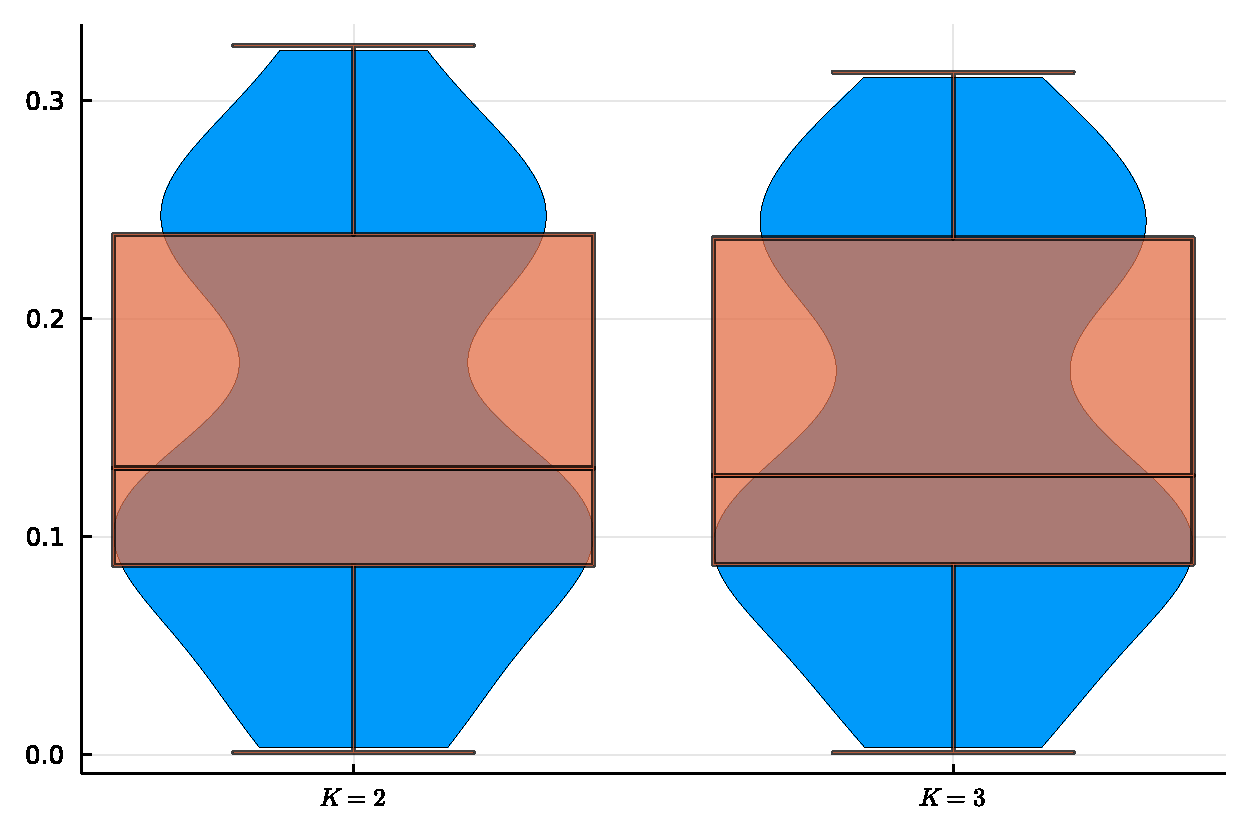
\includegraphics[scale=0.70]{../elexon/figures/2vs3_violin.pdf}
  \caption{Violin and box plots for likelihoods of the actualized residuals according to
  the estimated predictive distributions for the CEVMM models for $K=2$ and $K=3$.}\label{fig:k2_k3_violin}
\end{figure}


\begin{figure}[htp]
  \centering
  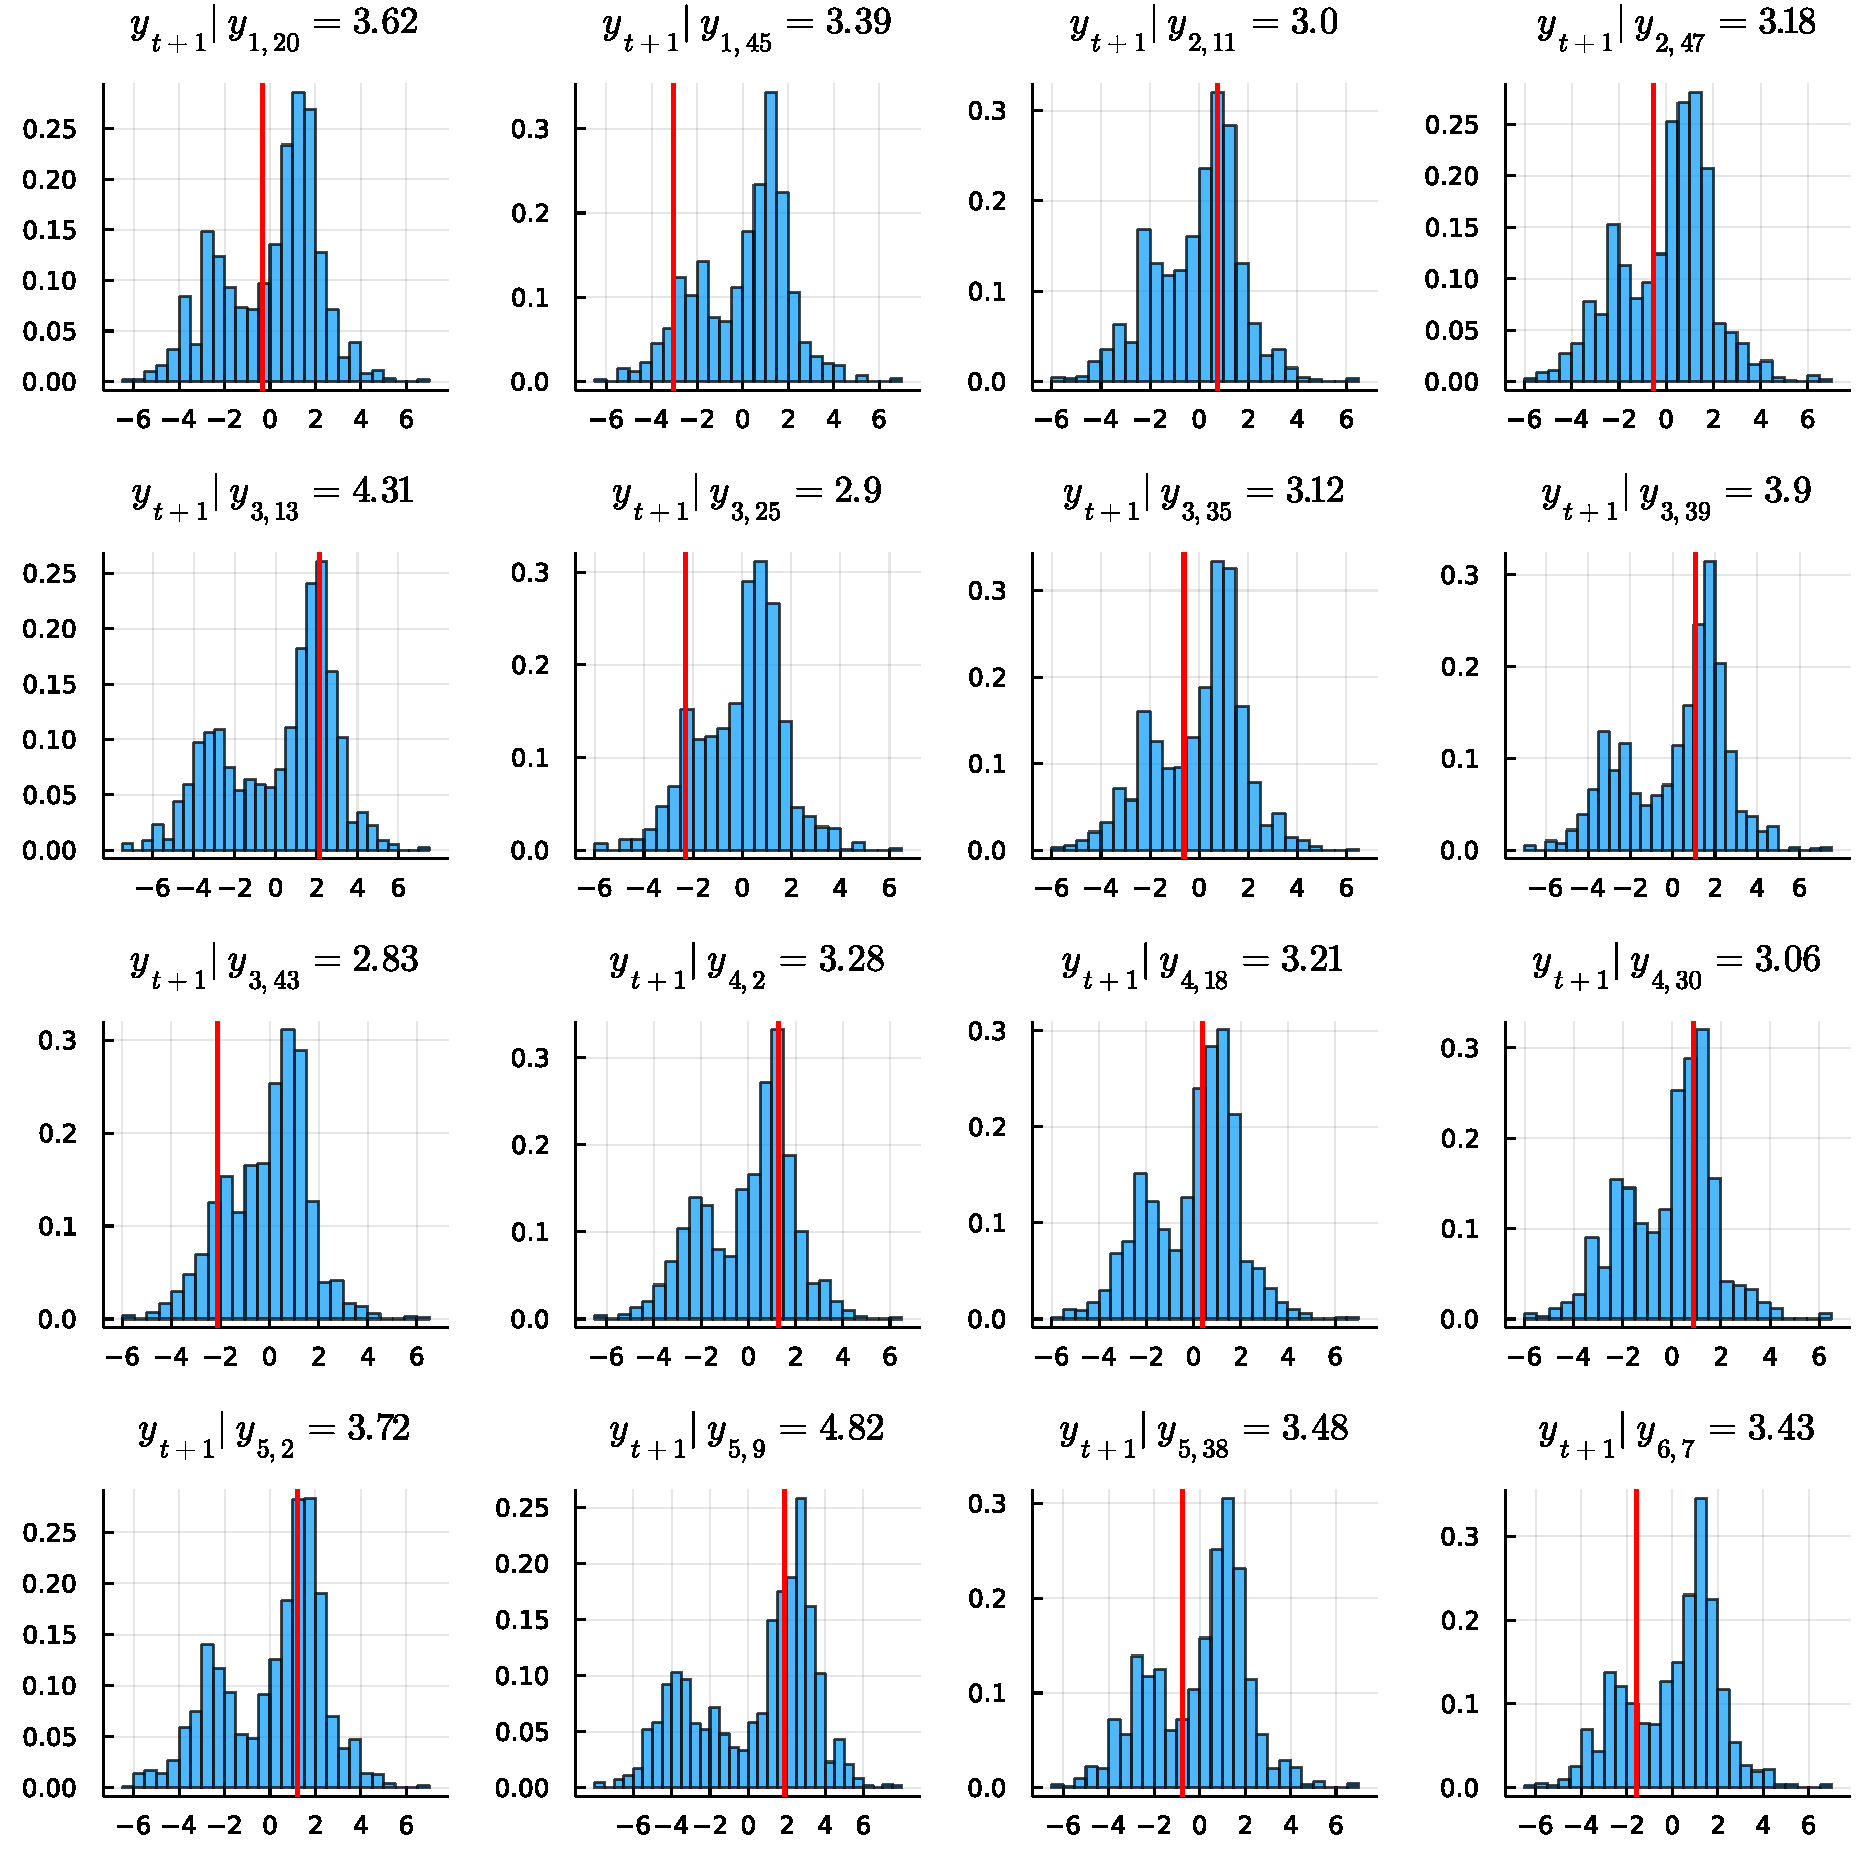
\includegraphics[scale=0.5]{../elexon/figures/ytp1_giv_yt_jan_22_Keq3.pdf}
  \caption{($K=3$) Histograms for simulated values of $y_{t+1}|y_{t}$ (here $y_{d,p}:=y_{48d - 1 + p}$ denotes the residual on day $d$ during period $p$ in January
    2022).
The red line shows the actualized value of $y_{t+1}$.}\label{fig:jan22_hists_k3}
\end{figure}



%Ultimately, predictions are not useful on this rather contrived Laplace scale,
%so we must transform them back to the scale of our original imbalance prices.
%According to the model, and using the notation from~\eqref{eq:seasonal_imbalance_price_factor}, we have

%\begin{equation}
  %\begin{split}
    %\code{log_price}_{t+1} &= \widehat{\code{log_price}}_{t+1} + y_{t+1}\\
    %\implies \code{price}_{t+1} &=
    %\exp\left(\text{sd}(\code{log_price'})
    %(\widehat{\code{log_price}}_{t+1} + y_{t+1}) + \text{mean}(\code{log_price'})\right) + \min \code{price} - 1
   %\end{split}
%\end{equation}

\FloatBarrier
\subsection{Conversion back to the original price scale}

While we have fitted the CEVMM on imbalance price residuals, this only provides
utility to electricity suppliers and producers if it is possible to frame the
results using GBP. In terms of one-step-ahead price prediction,
this can be done by first moving residuals from unit Laplace scale to their
original scale, and then applying~\eqref{eq:gbp_trans}.
  \begin{equation}\label{eq:gbp_trans}
  \begin{split}
    \code{log_price}_{t+1} &= \widehat{\code{log_price}}_{t+1} + y_{t+1}\\
    \implies \code{price}_{t+1} &=
    \exp\left(\text{sd}(\code{log_price'})
    (\widehat{\code{log_price}}_{t+1} + y_{t+1}) + \text{mean}(\code{log_price'})\right) - a
   \end{split}
\end{equation}

\begin{figure}[htp]
  \centering
  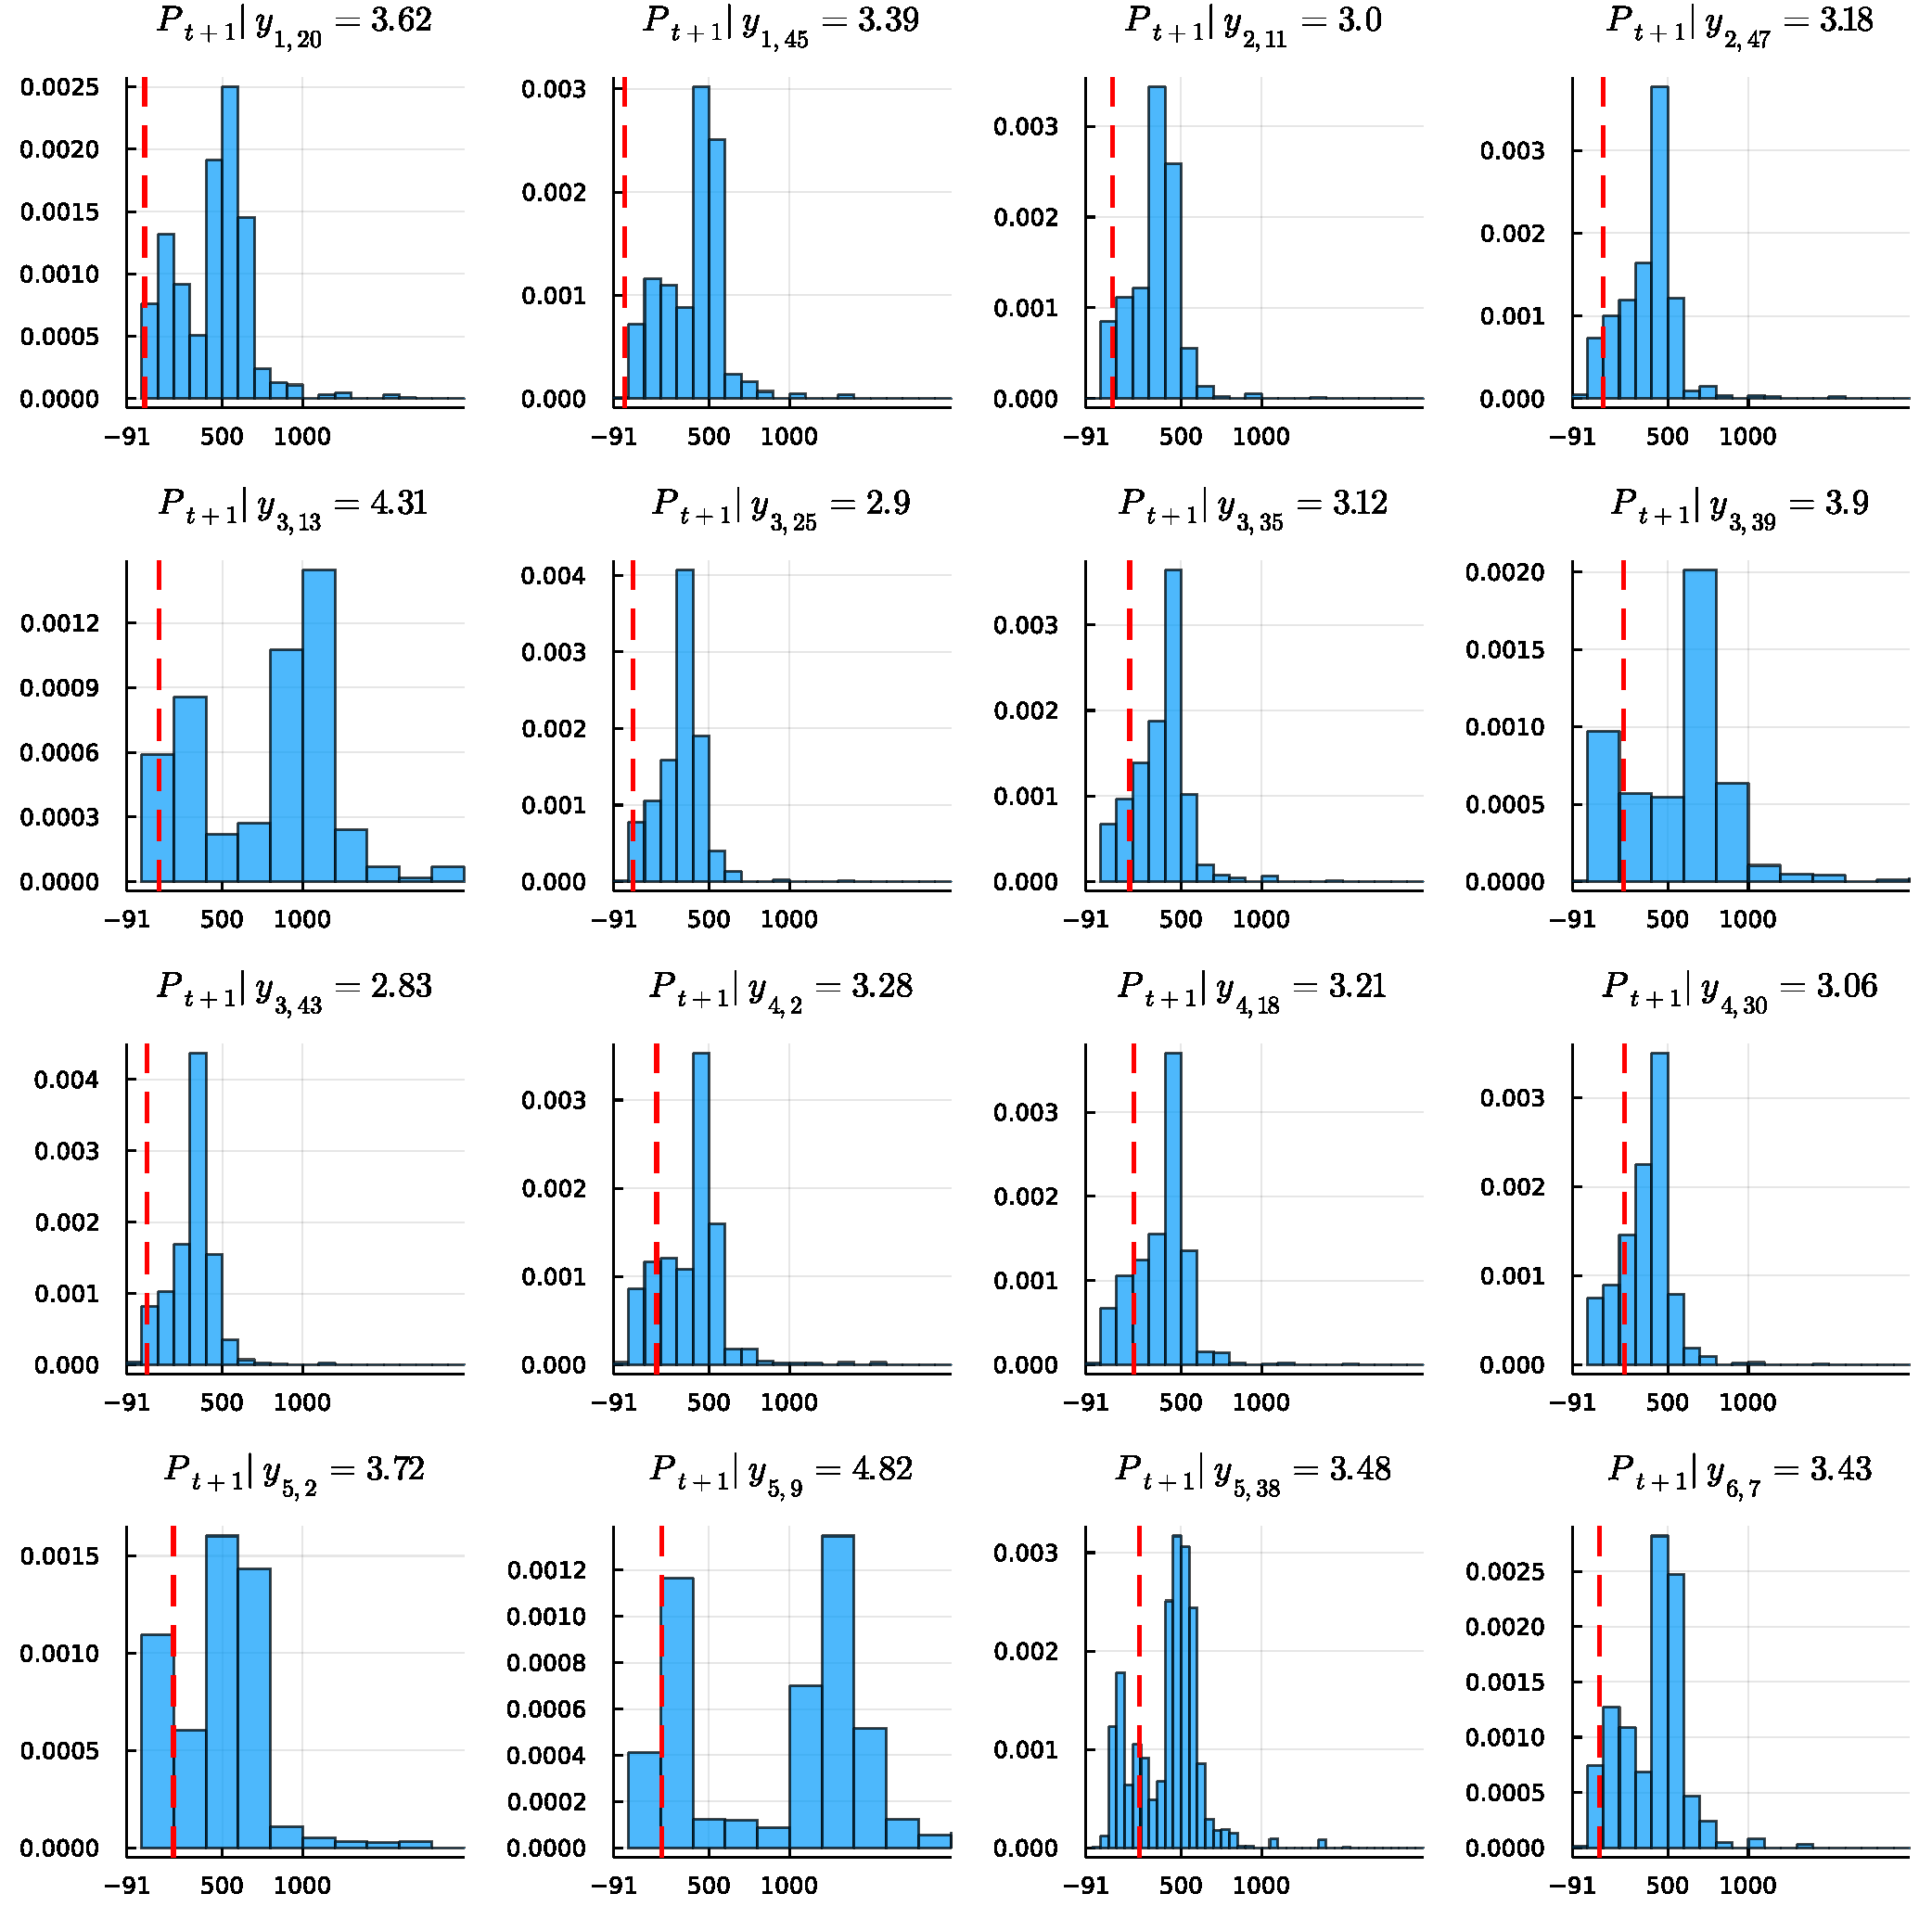
\includegraphics[scale=0.5]{../elexon/figures/price_preds_jan_22.pdf}
  \caption{Histograms for simulated values of $P_{t+1}|y_{t}$ under the CEVMM
    model~\ref{table:imb_reg05}. Here $y_{d,p}:=y_{48d - 1 + p}$ denotes the
    residual on day $d$ during period $p$ in January 2022, and $P_{t+1}|y_t$
    represents the imbalance price (measured in GBP) at time $t+1$, conditional
  on the previous period's imbalance residual. The red line shows the measured
value of $P_{t+1}$.}\label{fig:gbp_trans_hists}
\end{figure}


This reverse transform was applied to the predictive distributions of
Figure~\ref{fig:jan22_hists_22}, and the results can be found in
Figure~\ref{fig:gbp_trans_hists}. The results are underwhelming, most notably because the
predictive distributions suggest that high prices, around £500 are likely, but we
never see these actualized in the figure. This may be because the model
~\eqref{eq:select_imb_model} used to deseasonalize the imbalance prices is too
simplistic. It is also likely that a more sophisticated model is required to
perform accurate price prediction; one suggestion is to use CEVMM models
as part of a larger ensemble of models.

\FloatBarrier
\chapter{Conclusions}\label{sec:conclusion}

% what we have seen
We have developed and implemented the CEVMM model based on the EM algorithm,
and used it to characterize bivariate data. Models of this type have been
applied in the past, but the application here to stationary time series is
believed to be novel. Simulated data from a 3-dimensional asymmetric logistic
model was used to illustrate methods for fitting CEVMM models, assessing
uncertainty, and to validate the implementation. CEVMMs were
easily able to fit parameters that align closely with theoretical parameter values,
and we saw that the fitted distributions also aligned reasonably well, though
there was perhaps some bias.
We then considered electricity
imbalance price residuals, where there was evidence of extremal dependence. A
CEVMM model was fitted, and used to perform one-step-ahead residual prediction
with some success.

% advantages of the approach
Extreme events are rare by definition but can be catastrophic. Most statistical
and machine learning models are trained to fit to existing data, and are
therefore unlikely to be able to take these unlikely events into account
when making decisions.
CEVMMs however have the ability to shine in this domain.
By taking advantage of the theory of extremes that has been
developed over several decades, CEVMMs have the potential
to play a crucial role in managing this risk of extremes.
In their presented form, the CEVMM models discussed can be applied to any
bivariate dataset, under the mild assumption~\eqref{eq:htassump},
and also the assumption that exceedances are i.i.d.. The latter
is stringent in general, but is not unreasonable if we consider
datasets of consecutive pairs of realizations from stationary time series. It is
therefore expected
that CEVMM models will be broadly applicable, especially in fields
where stationary time series are prevalent.

While CEVMMs can be applied in the case of extremes, they
do not apply generally, and so to perform wholistic inference
it would be necessary to use them in tandem with other models,
which has not yet been investigated.
Additionally, whilst the methods proposed are relatively easy
to use, CEVMMs may rarely apply because they
are conditional on extreme values. This is not a problem directly,
but it makes model validation difficult as any test data is, by definition,
rare.

%Regarding the details of fitting CEVMMs, a Bayesian approach was not
%implemented here, but the EM algorithm demonstrated is expected to find similar
%point estimates when regularization is added, but in a much more
%computationally efficient manner. TODO benchmark

% weaknesses of the approach

% future work
There are several avenues for future work. Firstly, if CEVMMs were to be used
in tandem with other methods for wholistically modelling,
it is not obvious how this ought to be done. However, there is potential here.
For example, we saw that sometimes the CEVMM model was able to perform imbalance
residual prediction better than others; perhaps in the context of a larger
system, it would be possible to identify the times when the signal from the
CEVMM model is more reliable. Secondly, we have only demonstrated how CEVMMs
can be applied to bivariate data. It should be possible to extend the model to
the multivariate case (for example by repeating the methods shown to each extra
dimension, or even by adopting a multivariate normal model
in~\eqref{eq:ht_mix_fitting_step}). This could allow the development of
extremal models that take into account data from multiple stationary time
series, or that simply increase the number of consecutive data points used for
fitting beyond 2. Finally, there are many aspects regarding the implementation
that could be tested or improved. For example, construction of confidence
intervals was achieved with a moving block bootstrap, but it is not clear if
this is the best approach. Additionally, it is not understood how violation of
the i.i.d.\ assumption affects results; since this assumption can be
unrealistic for real data, it may be useful for practitioners to quantify the
tolerances here.




\bibliography{literature}

\appendix
\chapter{Appendices}


\section{EM algorithm for fitting conditional extremal $K$-mixture models with the normal assumption}
\label{appendix:htnormalem}

Let $\Phi(\cdot\,;\,\mu,\sigma^2)$ and $\phi(\cdot\,;\,\mu,\sigma^2)$
be the normal CDF and PDF respectively.
We are concerned with fitting the model
\begin{equation}\label{eq:htemnormalass}
    \p\left(Y\leq y | X =x\right) = \sum_{k=1}^K
    \pi_k \Phi_k\left(\frac{y - \alpha_1 x}{x^{\beta_k}};\mu_k,\sigma_k^2\right).
\end{equation}
We fit on a dataset
$\mathcal{D}=\{(x_i,y_i)\}_{i=1}^n$ where $x_i > u$ for some preferably large
$u$ ($u>0$ is strictly necessary for us to be able to evaluate fractional
powers of $x_i$), and it is assumed that elements of $\D$ are i.i.d.\ draws.
An EM
algorithm for finding $\pi$, $\alpha$, $\beta$, $\mu$, and $\sigma$ is
given in Algorithm~\ref{alg:normalht}.
\begin{algorithm}
\caption{EM algorithm for fitting conditional extremal $K$-mixture models with the normal assumption\label{alg:normalht}}
\begin{algorithmic}
\State Initialize a probability vector $\pi^{(0)}\in\mathcal{S}_K$
\State Initialize $\alpha_k^{(0)},\beta_k^{(0)}\in[0,1]$, $k=1,\ldots,K$.
\State Initialize $\mu_k^{(0)}\in\reals$, $k=1,\ldots,K$.
\State Initialize $\sigma_k^{(0)}\in\reals_{+}$, $k=1,\ldots,K$.
\State $t \gets 0$
\While{$\pi^{(t)},\alpha^{(t)},\beta^{(t)},\mu^{(t)},(\sigma^2)^{(t)}$ not all converged}
\For{$i \in 1,\ldots, n$} \Comment{E-step}
    \For{$k \in 1,\ldots, K$}
    \State $\tilde\pi_{ik}  \gets \frac{\pi^{(t)}_k \phi_k\left((y_i -  \alpha_k^{(t)}x_i)/x_i^{\beta_k^{(t)}};\mu_k,\sigma^2_k\right)}{\sum_{j=1}^K\pi^{(t)}_j
    \phi_j\left((y_i -  \alpha_j^{(t)})/x_i^{\beta_j^{(t)}};\mu_j,\sigma_j^2\right)}$
    \EndFor
  \EndFor
  \For{$k \in 1,\ldots, K$} \Comment{M-step}
  \State $\pi_k^{(t+1)} \gets \frac{1}{n}\sum_{i=1}^n \tilde\pi_{ik}$
  \EndFor
  \State $\alpha^{(t+1)},\beta^{(t+1)},\mu^{(t+1)},\sigma^{(t+1)}
  \gets\newline\hspace*{5em}\argmax_{\alpha,\beta,\mu,\sigma} \sum_{i=1}^n\sum_{k=1}^K\tilde\pi_{ik}\phi\left((y_i - \alpha_k x_i)/x_i^{\beta_k};\mu_k;\sigma_k^2 \right)$ \Comment{evaluated numerically}
  \State $t \gets t + 1$
\EndWhile
\State \Return $\pi^{(t)},\alpha^{(t)},\beta^{(t)},\mu^{(t)},\sigma^{(t)}$
\end{algorithmic}
\end{algorithm}

The method for calculating the $\argmax$ in Algorithm~\ref{alg:normalht} is
described in Section~\ref{sec:worked_example}. In particular, it is worth
emphasising that the reparameterization~\eqref{eq:htconstr} is used (it is easily
generalized to the general $K\in\mathbb{N}$ case). We also clarify what we mean
by convergence in Algorithm~\ref{alg:normalht}. We say $x^{(t)}$ has converged
if

\[
  \left|x^{(t)} - x^{(t-1)}\right| < \max\left\{\code{atol},\max\left\{\left|x^{(t)}\right|,\left|x^{(t-1)}\right|\right\} \code{rtol}\right\}
\]

with $\code{rtol}=\code{atol}=10^{-6}$.


\section{Constructing empirical CDFs in the CEVMM model}
\label{appendix:nonparametriccevmm}

This steps assumes that a normal $K$-mixture model~\eqref{eq:htemnormalass} has already been fit
and that fitting~\eqref{eq:cevmmnonpareq} is desired.


\begin{equation}\label{eq:cevmmnonpareq}
  \p\left(Y\leq y | X =x\right) = \sum_{k=1}^K
  \pi_k F^k_{\text{ecdf}}\left(\frac{y - \alpha_1 x}{x^{\beta_k}}\right)
\end{equation}

We take $\pi_k$, $\alpha_k$ and $\beta_k$ to be the fitted values from Algorithm~\ref{alg:normalht},
and then use Algorithm~\ref{alg:resids}, as described in~\cite{tendijck2021modeling}, to sample
residuals $Z_1,\,\ldots,\,Z_K$.

\begin{algorithm}
\caption{Sample residuals in the CEVMM model\label{alg:resids}}
\begin{algorithmic}
\State Assumes $\hat\alpha,\hat\beta\in[0,1]^K$, $\hat\pi\in\mathcal{S}_K$, $\hat\mu\in\reals^K$, $\hat\sigma\in\reals_{+}^K$.
\State Initialize $M$\Comment{\# of samples}
\State Initialize empty arrays $Z_1,\,\ldots,\,Z_K$\Comment{Residuals}
\For{$i \in 1\,,\,\ldots\,,\, n$}\Comment{Calculate mixture probabilities for each data point}
    \For{$k \in 1\,,\ldots\,, K$}
    \State $\tilde\pi_{ik}  \gets \frac{\hat\pi_k \phi_k\left((y_i -  \hat\alpha_kx_i)/x_i^{\hat\beta_k}\,;\,\hat\mu_k,\hat\sigma^2_k\right)}{\sum_{j=1}^K\hat\pi_j
    \phi_j\left((y_i -  \hat\alpha_j)/x_i^{\hat\beta_j}\,;\,\hat\mu_j,\hat\sigma_j^2\right)}$
    \EndFor
  \EndFor
  \For{$m \in 1,\ldots, M$}
    \For{$i \in 1,\,\ldots,\,n$}
    \State $C \gets \text{ sample from Categorical}\left((\pi_{ik})_{k\in\{1,\,\ldots,\, K\}}\right)$
    \State Append $\frac{y_i - \hat\alpha_C x_i}{x_i^{\hat\beta_C}}$ onto array $Z_C$
    \EndFor
  \EndFor
\State \Return $Z_1,\,\ldots,\,Z_K$
\end{algorithmic}
\end{algorithm}

After running Algorithm~\ref{alg:resids}, the estimators become

\[
  \hat F^k_{\text{ecdf}}(x) = \frac{1}{|Z_k|}\sum_{j=1}^{|Z_k|} 1\left((Z_k)_j \leq x\right),
\]

where $1(\cdot)$ is the indicator function. The normal assumption,
$\hat\mu$ and $\hat\sigma$ are then discarded.

%\section{Deseasonalizing electricity imbalance prices: stepwise selection output}
%\label{appendix:nonparametriccevmm}

%\begin{figure}[htp]
  %\centering
  %\begin{minted}{r}
%## perform stepwise selection on a 'large' model
%m <- lm(log_price ~  yday_log_price*yday_quantity +
                     %last_log_price1*last_quantity1 +
                     %last_log_price2*last_quantity2 +
                     %period + month +
                     %weekday,
        %data=df)
%step(m)

%## output
%<snip>
%Step:  AIC=-18861.04
%log_price ~ yday_log_price + last_log_price1 + last_quantity1 +
    %last_log_price2 + last_quantity2 + period + month + weekday +
    %last_log_price2:last_quantity2

                                 %Df Sum of Sq    RSS    AIC
%<none>                                        5888.3 -18861
%- last_log_price2:last_quantity2  1      3.33 5891.7 -18853
%- weekday                         6     13.18 5901.5 -18834
%- yday_log_price                  1     33.68 5922.0 -18763
%- period                         47    162.31 6050.6 -18480
%- last_quantity1                  1    144.95 6033.3 -18438
%- month                          11    248.95 6137.3 -18160
%- last_log_price1                 1    950.33 6838.7 -16249
%\end{minted}
  %\caption{Stepwise selection with AIC criterion and its output.}\label{fig:stepwise_output_lm}
%\end{figure}

\end{document}
